\documentclass[8pt]{scrartcl}

% === Page Layout ===
\usepackage[a4paper,margin=1.2in]{geometry}
\usepackage{setspace}
\usepackage{natbib}
\usepackage{float}
\usepackage{longtable}
\usepackage{xcolor}
\usepackage{tcolorbox}
\usepackage{multicol}
\onehalfspacing

% === Fonts & Typography ===
\usepackage{lmodern}
\usepackage{times}

\usepackage{paralist}
  \let\itemize\compactitem
  \let\enditemize\endcompactitem
  \let\enumerate\compactenum
  \let\endenumerate\endcompactenum
  \let\description\compactdesc
  \let\enddescription\endcompactdesc
  \pltopsep=1pt
  \plitemsep=1pt
  \plparsep=1pt


% === Graphics & Formatting ===
\usepackage{graphicx}
\usepackage{booktabs}
\usepackage{float}

% === Code Listings ===
\usepackage{listings}

% === Hyperlinks ===
\usepackage{hyperref}
\hypersetup{
    colorlinks=true,
    linkcolor=blue,
    citecolor=blue,
    urlcolor=blue
}

% === Headers & Footers ===
\usepackage{scrlayer-scrpage}
\pagestyle{scrheadings}
\ihead{Expert Evaluation of LLM-Generated Trade Strategies}
\ohead{\thepage}
\cfoot{}

% === Title & Author ===
\title{Expert Evaluation of LLM-Generated Trade Strategies}
\author{Adam Darmanin}
\date{January 2025}

\AtBeginDocument{%
  \providecommand\BibTeX{{%
    Bib\TeX}}}

\begin{document}

\maketitle

\section{Introduction}

This document outlines a structured methodology for expert reviewers to evaluate trade strategies generated by Large Language Models (LLMs). The evaluation framework is based on principles from Reinforcement Learning from Human Feedback (RLHF) \citep{Retzlaff2024HumanintheLoopRL} and Human-AI Teaming \citep{vats2024surveyhumanaiteaminglarge, xie2024text2rewardrewardshapinglanguage}.

The goal is to assess whether AI-generated strategies are logical, aligned with what portfolio managers would do, and safe for real-world application. The expert’s role is to score, annotate, and, where possible, provide exemplar corrections.

The findings from this evaluation will contribute to the paper: "Language Model Guided Reinforcement Learning in Quantitative Trading." Reviewers will be acknowledged for their contributions, and the results will be shared.

\section{Review Instructions}

\subsection{Step 1: Problem Definition}

You will be provided with one year of historical market data, the data is anonymized to prevent bias due to prior knowledge of the financial instrument:
\begin{enumerate}
    \item Price and volatility trends (e.g. Weekly Close, Otions IV, Moving Averages),
    \item Fundamental indicators (e.g., Cash Flow, P/E ratio),
    \item Economic indicators (e.g., Consumer Confidence, PPI),
    \item Anonymized news summaries related to the trading instrument.
\end{enumerate}

Your first task is to analyze the given information and determine the likely optimal trading action: \textit{LONG} (buy) or \textit{SHORT} (sell) with a brief justification (one or two sentences) for your chosen position.

\subsection{Step 2: Expert Scoring}

Next, you will evaluate the LLM-generated trade strategy by analyzing its decision \textit{rationale} \citep{vats2024surveyhumanaiteaminglarge} and \textit{selection of key influencing factors} \citep{wang2024llmfactorextractingprofitablefactors}. The scores are defined in the rubric below, inspired by Explainable AI (XAI) metrics \citet{Demajo_2020, xai_Khawaga_2023}:

\begin{table}[H]
\centering
\renewcommand{\arraystretch}{1.2} % Increase row spacing for readability
\begin{tabular}{p{2.55cm} p{4.25cm} p{4.25cm} p{4.25cm}} % Adjust column widths
\toprule
\textbf{Criterion} & \textbf{Score -1 (Poor)} & \textbf{Score 0 (Average)} & \textbf{Score 1 (Good)} \\
\midrule
\textbf{Rationale} & Contradicting and/or with logical errors. & Mostly coherent, with some gaps. & Logical and valid reasoning. \\
\textbf{Fidelity} & Not applicable to real-world markets. & Somewhat applicable, but unrealistic. & Performs like a trained professional. \\
\textbf{Safety} & Ignored the risks. & Recognized the risks but did not act. & Recognized and mitigated the risks. \\
\bottomrule
\end{tabular}
\caption{Scoring rubric for expert evaluations.}
\label{tab:scoring}
\end{table}


\subsection{Step 3: Expert Exemplars}

After scoring the AI's decision, and if applicable, you are requested to provide specific feedback on errors in the form of corrective explanations \citep{xie2024text2rewardrewardshapinglanguage}. You can skip this if the model was perfect, or there is no root cause in the historic market data for causing the model to fail (e.g. a black swan event).

\textbf{Guidelines for Expert Feedback:}
\begin{enumerate}
    \item Identify where the AI's decision deviates from sound trading principles.
    \item Provide a corrected response that aligns with best market practices.
\end{enumerate}

An example of a corrective explanation:
\begin{quote}
    \textbf{LLM's Explanation:} "Degrading fundamentals on TSLA, with a decrease in consumer confidence, suggest a \textit{SHORT} position." \\
    \textbf{Expert's Explanation:} The high ATR range of TSLA, coupled with an increase in implied volatility (IV) on call options, and the CEO’s optimistic guidance in a recent interview, indicates a potential \textit{LONG} setup despite the market downturn.
\end{quote}

\subsection{Step 4: Iterative Refinement}

The feedback, scores, and exemplars provided by experts will be collected to refine and improve the AI’s decision-making process similar to Reinforcement Learning from Human Feedback (RLHF) \cite{Retzlaff2024HumanintheLoopRL, Pternea_2024}.

\subsection*{Understanding the Data and Key Terminology}

This section provides explanations for the data you will encounter. If you are confident skip to the first strategy sample (Section~\ref{app:s1}).

\begin{multicols}{2}

\textbf{Macroeconomic Indicators:}
\begin{enumerate}
    \item \textit{GDP (Gross Domestic Product)}: Measures economic growth; higher values indicate expansion.
    \item \textit{PMI (Purchasing Managers' Index)}: Above 50 signals growth, below 50 signals contraction.
    \item \textit{PPI (Producer Price Index)}: Tracks inflation at the wholesale level; rising PPI may indicate cost pressures.
    \item \textit{Treasury Yields}: Reflect borrowing costs and impact equity valuations.
    \item \textit{Yield Curve}: An inverted yield curve can signal recession risks.
    \item \textit{Consumer Confidence}: Measures sentiment; higher values indicate optimism in economic conditions.
\end{enumerate}

\textbf{Market Volatility and Options:}
\begin{enumerate}
    \item \textit{Implied Volatility (IV)}: Predicts future price swings; higher IV means more uncertainty.
    \item \textit{VIX (Volatility Index)}: Measures market risk and investor sentiment.
    \item \textit{Options Skew}: Identifies sentiment shifts; rising put skew suggests bearish sentiment.
    \item \textit{ATM (At-The-Money) \& OTM (Out-Of-The-Money)}: Define option pricing relative to the stock price.
\end{enumerate}

\textbf{Technical Indicators:}
\begin{enumerate}
    \item \textit{Relative Strength Index (RSI)}: Above 70 indicates overbought conditions, below 30 suggests oversold.
    \item \textit{MACD (Moving Average Convergence Divergence)}: Tracks momentum shifts using moving averages.
    \item \textit{VWAP (Volume Weighted Average Price)}: Determines fair price levels based on trading volume.
    \item \textit{Bollinger Bands}: Measure price volatility around a moving average.
\end{enumerate}

\textbf{Fundamental Indicators:}
\begin{enumerate}
    \item \textit{Earnings Per Share (EPS)}: Indicates profitability per share.
    \item \textit{Price-to-Earnings (P/E) Ratio)}: High values suggest growth expectations.
    \item \textit{Net Profit Margin}: Measures earnings efficiency; higher margins indicate strong profitability.
    \item \textit{Debt-to-Equity Ratio}: Highlights financial leverage, with higher values indicating greater debt reliance.
\end{enumerate}

\end{multicols}

Also in the models output and performance metrics, you will see the following terms.

\begin{multicols}{2}

\textbf{LLM Metrics:}
\begin{enumerate}
    \item \textit{Perplexity (PPL)}: Measures model uncertainty; lower values indicate better confidence in the strategy \cite{gonen-etal-2023-demystifying}.
    \item \textit{Strategy Probabilities}: The evaluator's calculated probabilities for a LONG or SHORT.
    \item \textit{Total Token}: The number of tokens used between agents to create the strategy.
    \item \textit{Total Cost}: The cost of generating the strategy, depending on the model used.
\end{enumerate}

\textbf{Portfolio Metrics:}
\begin{enumerate}
    \item \textit{Sharpe Ratio}: Risk-adjusted return metric; higher values indicate better efficiency.
    \item \textit{Max Drawdown}: Measures the largest drop in portfolio value from peak to trough.
    \item \textit{Cumulative Returns}: Tracks overall portfolio growth over time.
\end{enumerate}

\end{multicols}

\section{Conclusion}

This structured expert review framework ensures that LLM-generated trade strategies are evaluated for safety, logical consistency, and market relevance. The findings from this evaluation will contribute to the paper: "Language Model Guided Reinforcement Learning in Quantitative Trading.".

Review sheet and samples are provided in the appendix. Start with sample 1~\ref{app:s1}.

\bibliographystyle{ACM-Reference-Format}
\bibliography{refs}

\newpage

\appendix
\section*{Review Sheet}
\label{app:Review_Sheet}

You will be filling the accompanying spreadsheet. This is for reference only

\begin{table}[h]
    \centering
    \renewcommand{\arraystretch}{1.3}
    \setlength{\tabcolsep}{5pt}
    \resizebox{\textwidth}{!}{%
    \begin{tabular}{|c|c|p{3.5cm}|c|c|c|p{3.5cm}|}
        \hline
        \textbf{Sample ID} & \textbf{Expert's Guess} & \textbf{Expert's Rationale} & \textbf{Model Rationale (-1 to 1)} & \textbf{Model Fidelity (-1 to 1)} & \textbf{Model Safety (-1 to 1)} & \textbf{Expert's Exemplar} \\
        \hline
        1  &  &  &  &  &  &  \\
        \hline
        2  &  &  &  &  &  &  \\
        \hline
        3  &  &  &  &  &  &  \\
        \hline
        4  &  &  &  &  &  &  \\
        \hline
        5  &  &  &  &  &  &  \\
        \hline
        6  &  &  &  &  &  &  \\
        \hline
        7  &  &  &  &  &  &  \\
        \hline
        8  &  &  &  &  &  &  \\
        \hline
        9  &  &  &  &  &  &  \\
        \hline
        10 &  &  &  &  &  &  \\
        \hline
    \end{tabular}
    }
    \caption{Expert Review Sheet}
\end{table}

\newpage

\section*{LLM Strategy 1}
\label{app:s1}

\subsection*{Historic 1 Year Data}

\begin{figure}[H]
    \centering
    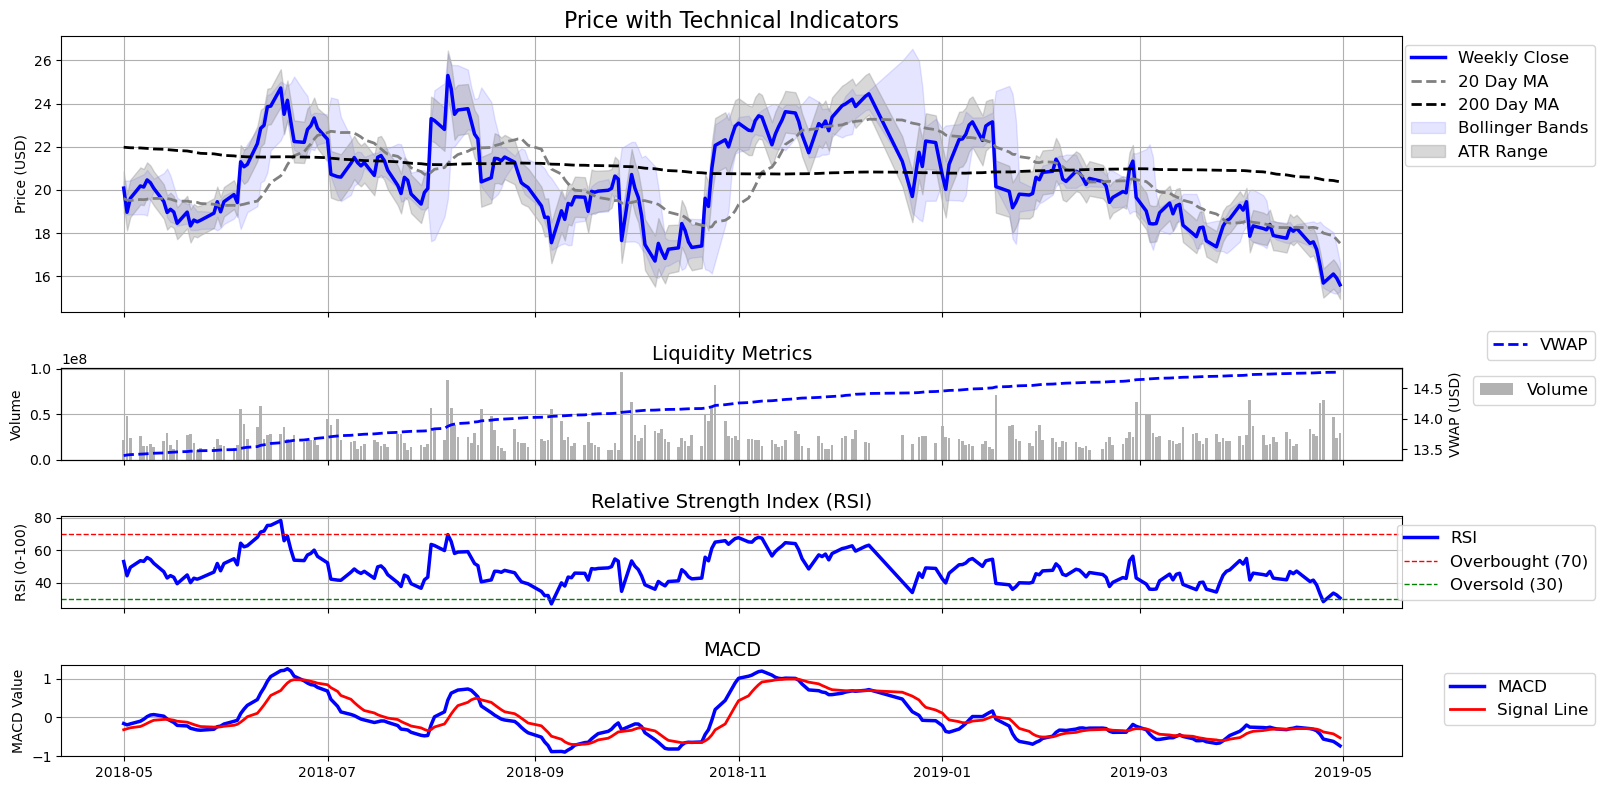
\includegraphics[width=1\linewidth]{judge_reviews//TSLA_M_gpt-4o-mini//2019-05-01/judge_Price_with_Technical_Indicators.png}
    \caption{Price and Technicals}
\end{figure}

\begin{figure}[H]
    \centering
    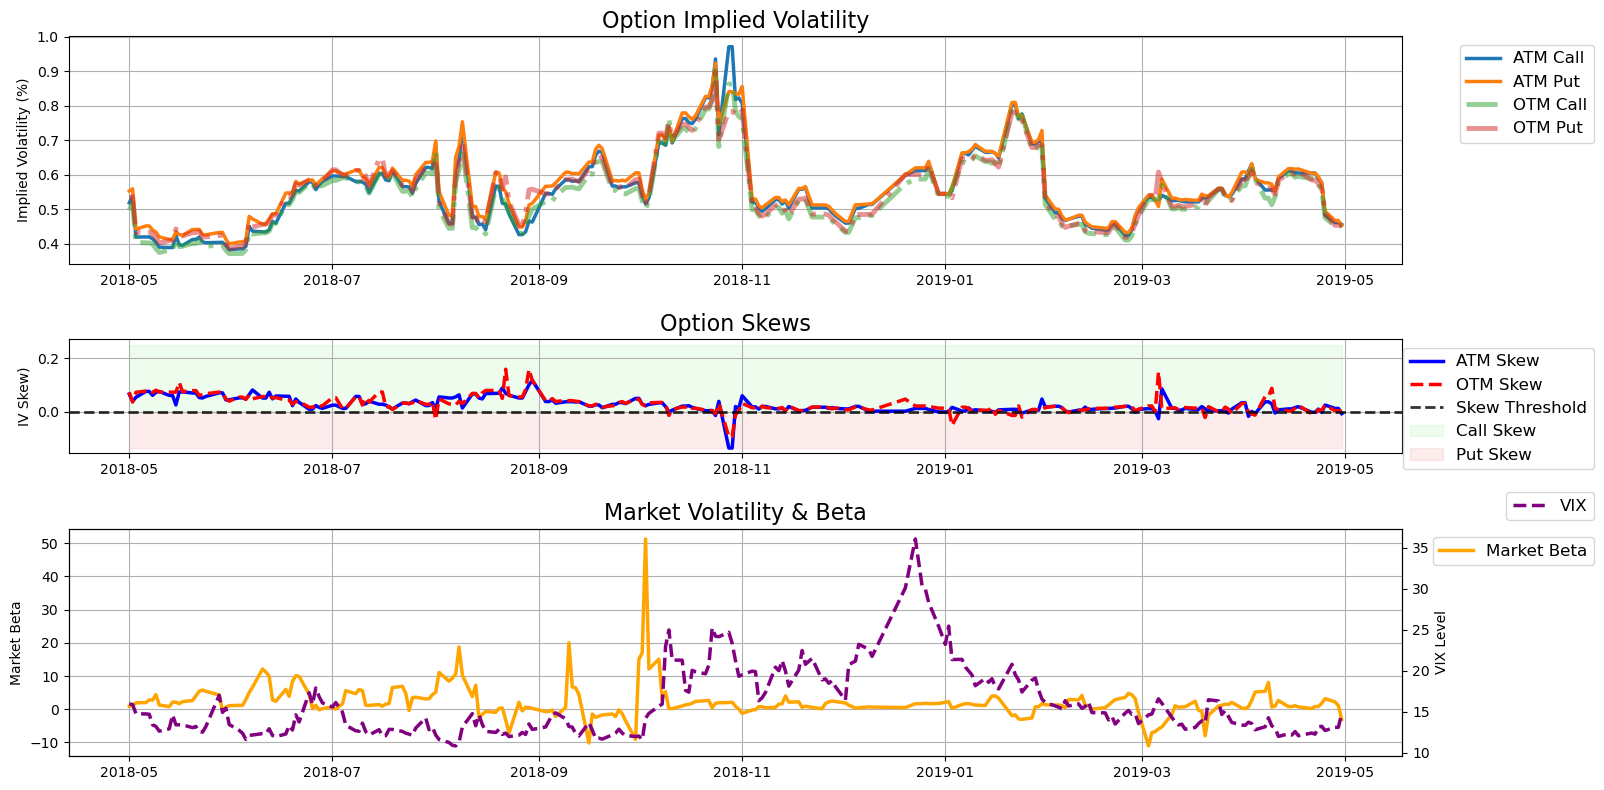
\includegraphics[width=1\linewidth]{judge_reviews/TSLA_M_gpt-4o-mini/2019-05-01/judge_Option_Implied_Volatility.png}
    \caption{Options}
\end{figure}

\begin{figure}[H]
    \centering
    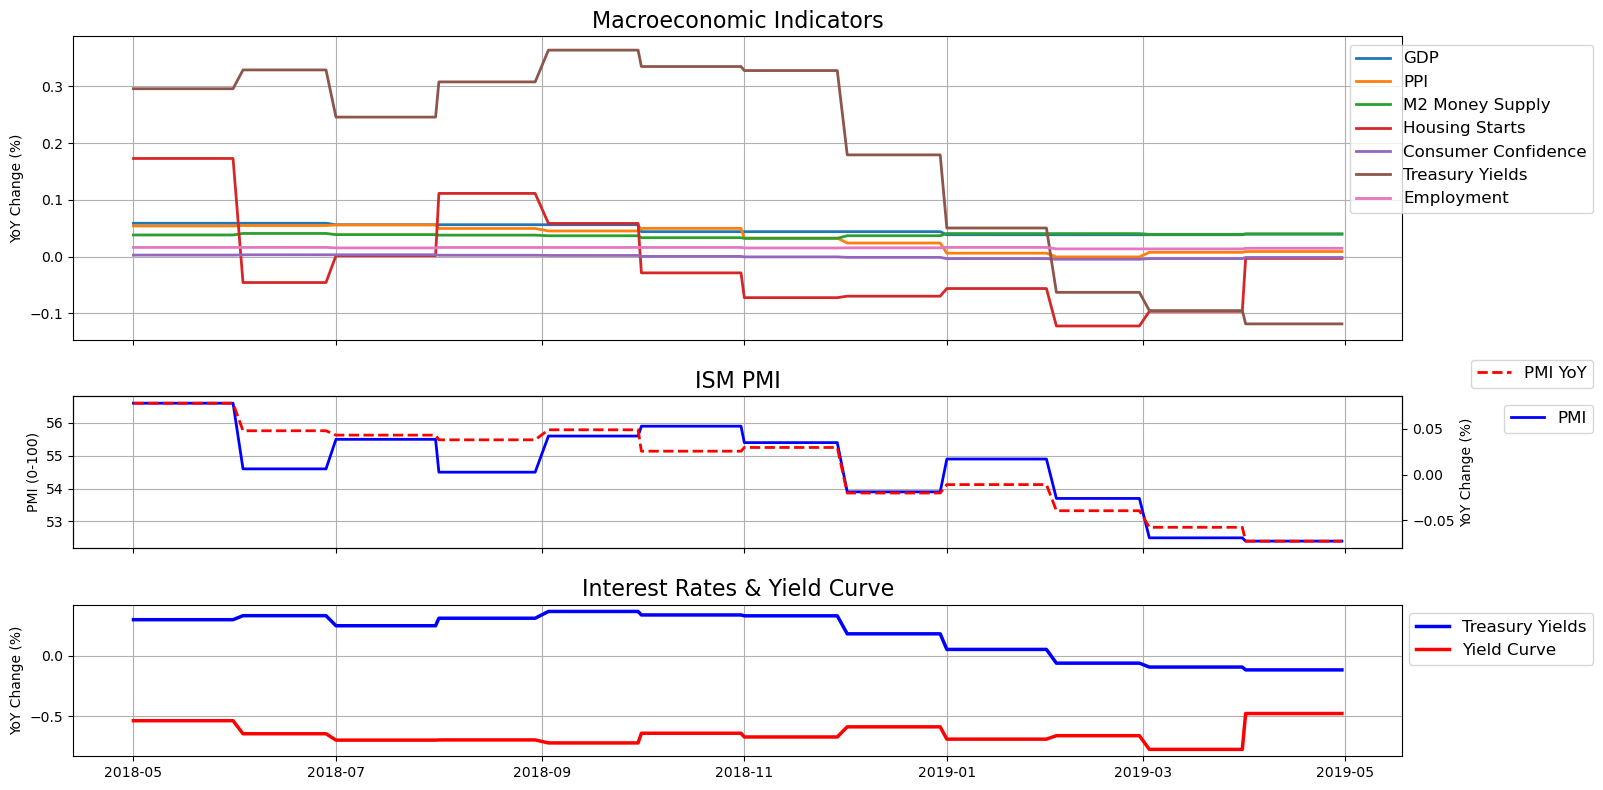
\includegraphics[width=1\linewidth]{judge_reviews/TSLA_M_gpt-4o-mini/2019-05-01/judge_Macroeconomic_Indicators.png}
    \caption{Macroeconomic}
\end{figure}

\begin{figure}[H]
    \centering
    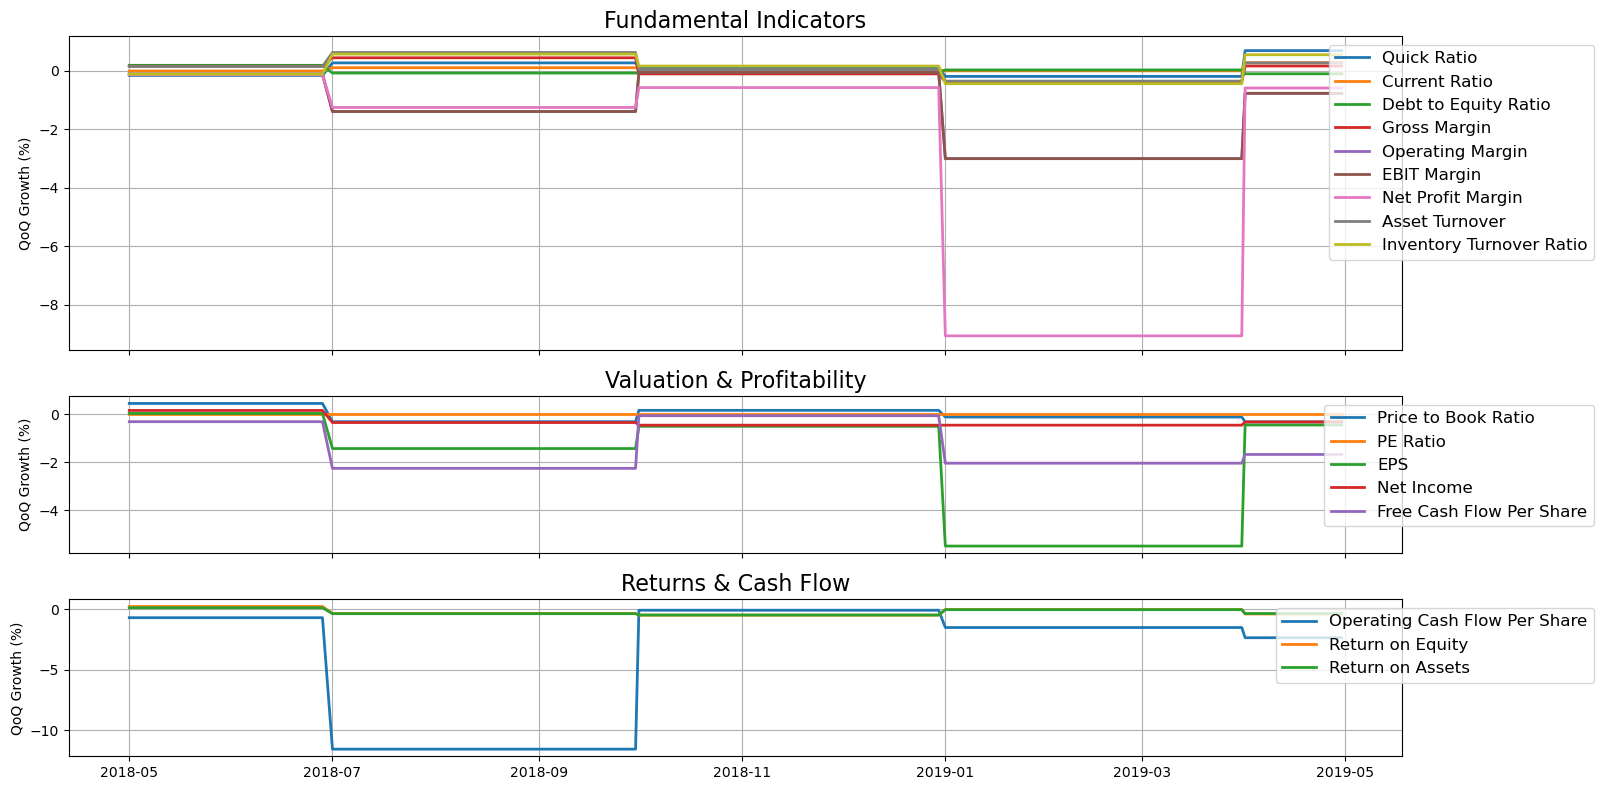
\includegraphics[width=1\linewidth]{judge_reviews/TSLA_M_gpt-4o-mini/2019-05-01/judge_Fundamental_Indicators.png}
    \caption{Fundamentals}
\end{figure}


\subsection*{Historic 1 Month News}

\textbf{Board Restructuring \& Corporate Governance Changes}
THE COMPANY announced plans to streamline its board by reducing the number of directors and changing voting procedures. Some investors saw this as a positive step toward improved corporate governance, while others expressed concerns about reducing independent oversight. The impact on THE COMPANY's stock was initially neutral to slightly negative.

\textbf{Vehicle Fire Incident in China}
A viral video showed a parked vehicle from THE COMPANY spontaneously combusting in China. This incident triggered strong reactions from Chinese consumers and raised concerns about vehicle safety, particularly in a key market where THE COMPANY is trying to expand. The news contributed to a stock decline and added pressure on its reputation.

\textbf{Autonomous Driving \& Robotaxi Claims}
THE CEO made bold claims about launching fully autonomous taxis by next year, stating that owning any other vehicle would soon be "financially insane." While some analysts acknowledged THE COMPANY's leadership in electric vehicles, others viewed the announcement as an attempt to distract from operational challenges. Investors were skeptical, and the stock reaction remained muted.

\textbf{Disappointing Earnings Report}
THE COMPANY reported worse-than-expected financial results, missing both revenue and earnings estimates. Vehicle deliveries declined, cash reserves fell, and the outlook for profitability weakened. Analysts downgraded the stock, citing concerns over demand, production efficiency, and capital requirements. The stock dropped following the earnings release.

\textbf{Capital Raise Speculation}
Following the earnings report, analysts predicted that THE COMPANY would need to raise additional funds to sustain operations and growth. THE CEO initially resisted the idea but later acknowledged its potential necessity. This uncertainty around financing created volatility in the stock and raised concerns about long-term financial stability.


\begin{tcolorbox}[colback=blue!10, colframe=blue!60, title=\textbf{TASKS}, sharp corners=southwest]
\begin{enumerate}
    \item Guess the action to take: \textit{LONG} or \textit{SHORT}.
    \item Write a 1-2 sentence \textit{explanation} on why you decided the action above.
\end{enumerate}
\end{tcolorbox}

\textbf{NEXT PAGE}: Model's Decision and Rationale.

\newpage

\subsection*{LLMs' Strategy} \label{strategy1}

The traded instrument was TSLA, with the trading period set between 2019-05-05 and 2019-06-02.

\textbf{LLMs' decision: \textit{SHORT}}

\textbf{Rationale}: The analysis suggests a SHORT position due to several concerning factors. Firstly, the company's fundamental metrics are weak, with negative EPS YoY (-46.43\%), Free Cash Flow YoY (-183.06\%), and Net Income YoY (-75.37\%). These figures indicate declining profitability and cash flow issues, which undermine confidence in future earnings growth.

Secondly, the technical indicators reveal bearish signals: the stock is currently trading below its 50MA (19.52) and 200MA (20.89), suggesting that momentum is shifting downward. The MACD shows a bearish strength (-0.286) while RSI sits at 51, indicating neutral but potential weakness ahead.

Furthermore, news factors highlight significant risks: analysts have downgraded the stock rating from Outperform to Peer Perform due to concerns over demand for its flagship product—an indication of weakening consumer interest amidst increasing competition in the electric vehicle market.

\textbf{Top weighted features influencing this decision}:
\begin{enumerate}
    \item Stock\_Data.Price.Close (19.06)
    \item Technical\_Analysis.MACD.Value (-0.286)
    \item Fundamental\_Data.Growth\_Metrics.EPS\_YoY (-46\%)
    \item Fundamental\_Data.Growth\_Metrics.Free\_Cash\_Flow\_YoY (-183\%)
    \item Options\_Data.Put\_IV\_Skews.Otm\_Skew (1.05)
\end{enumerate}

\textbf{Key news impacting this strategy}:
\begin{enumerate}
    \item Analysts’ downgrade on performance - Market Impact Score: 5/5
    \item CEO’s share purchase showing confidence amid uncertainties - Market Impact Score: 4/5
    \item Fatal crash raising safety concerns leading to regulatory scrutiny - Market Impact Score: 4/5
\end{enumerate}

\textbf{LLM Decision Insights}

\begin{longtable}{l c}
\toprule
\textbf{LLM Decision Insights} & \textbf{Value} \\
\midrule
Long Probability & 0.1 \\
Short Probability & 0.9 \\
Perplexity & 1.86614   \\
\midrule
Total Tokens & 19627 \\
Total Cost (USD) & \$0.003212 \\
\bottomrule
\end{longtable}


\subsection*{Following Month Data}

\textbf{Performance Metrics}

\begin{longtable}{l c}
\toprule
\textbf{Metric} & \textbf{Value} \\
\midrule
Sharpe Ratio (Annualized SR) & 7.35114 \\
Portfolio Turnover (PTR) & 0 \\
Maximum Drawdown (MDD) & 0.0459915 \\
Mean Drawdown Duration (MDDur) & 2 \\
Cumulative Returns & 0.294539 \\
\bottomrule
\end{longtable}

\begin{figure}[H]
    \centering
    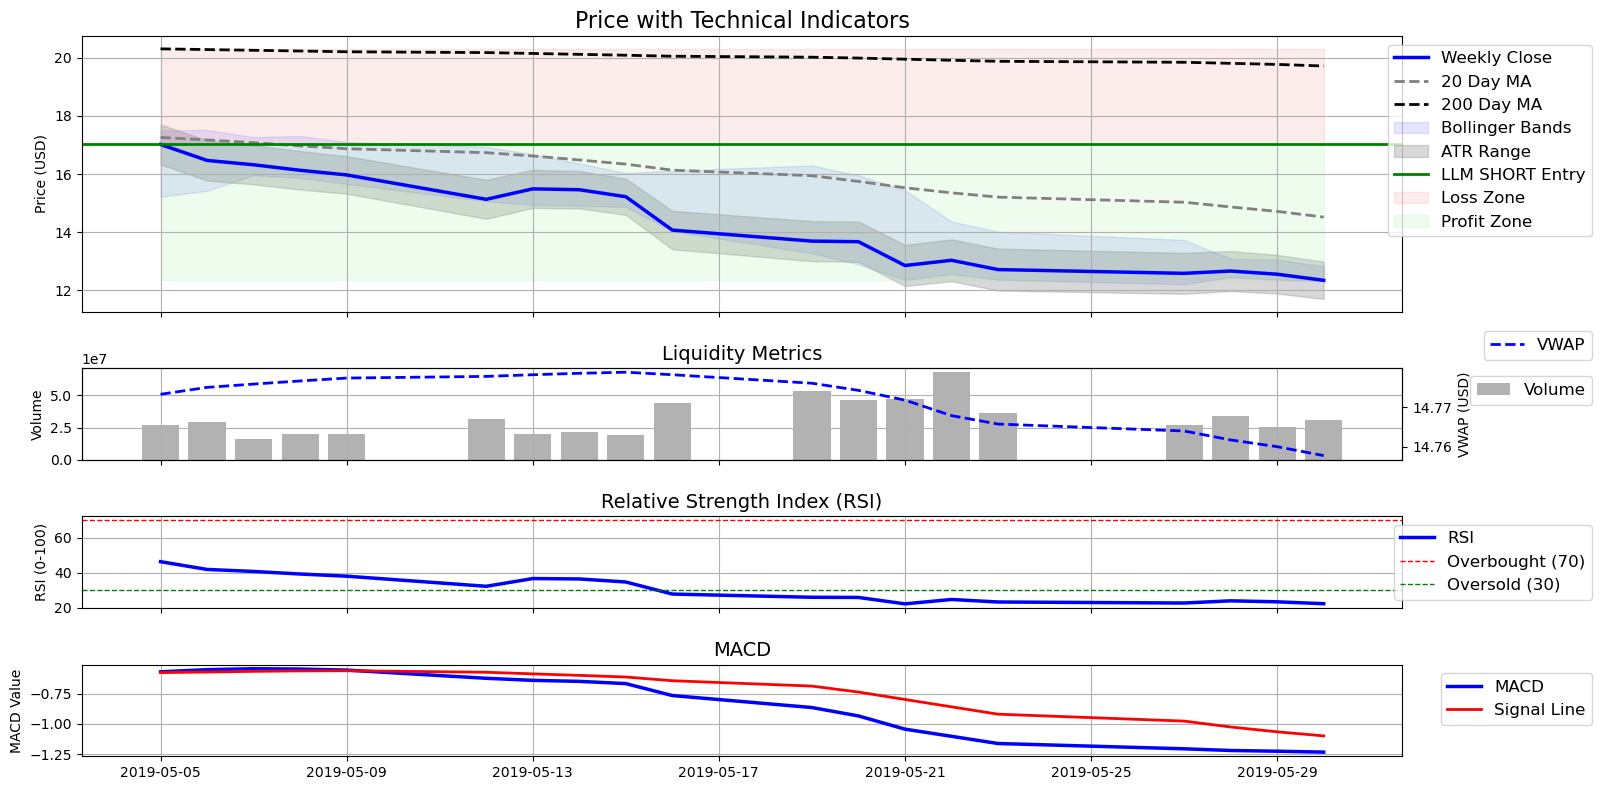
\includegraphics[width=1\linewidth]{judge_reviews//TSLA_M_gpt-4o-mini//2019-05-01/llm_Price_with_Technical_Indicators.png}
    \caption{Price after LLM's decision}
\end{figure}

\begin{figure}[H]
    \centering
    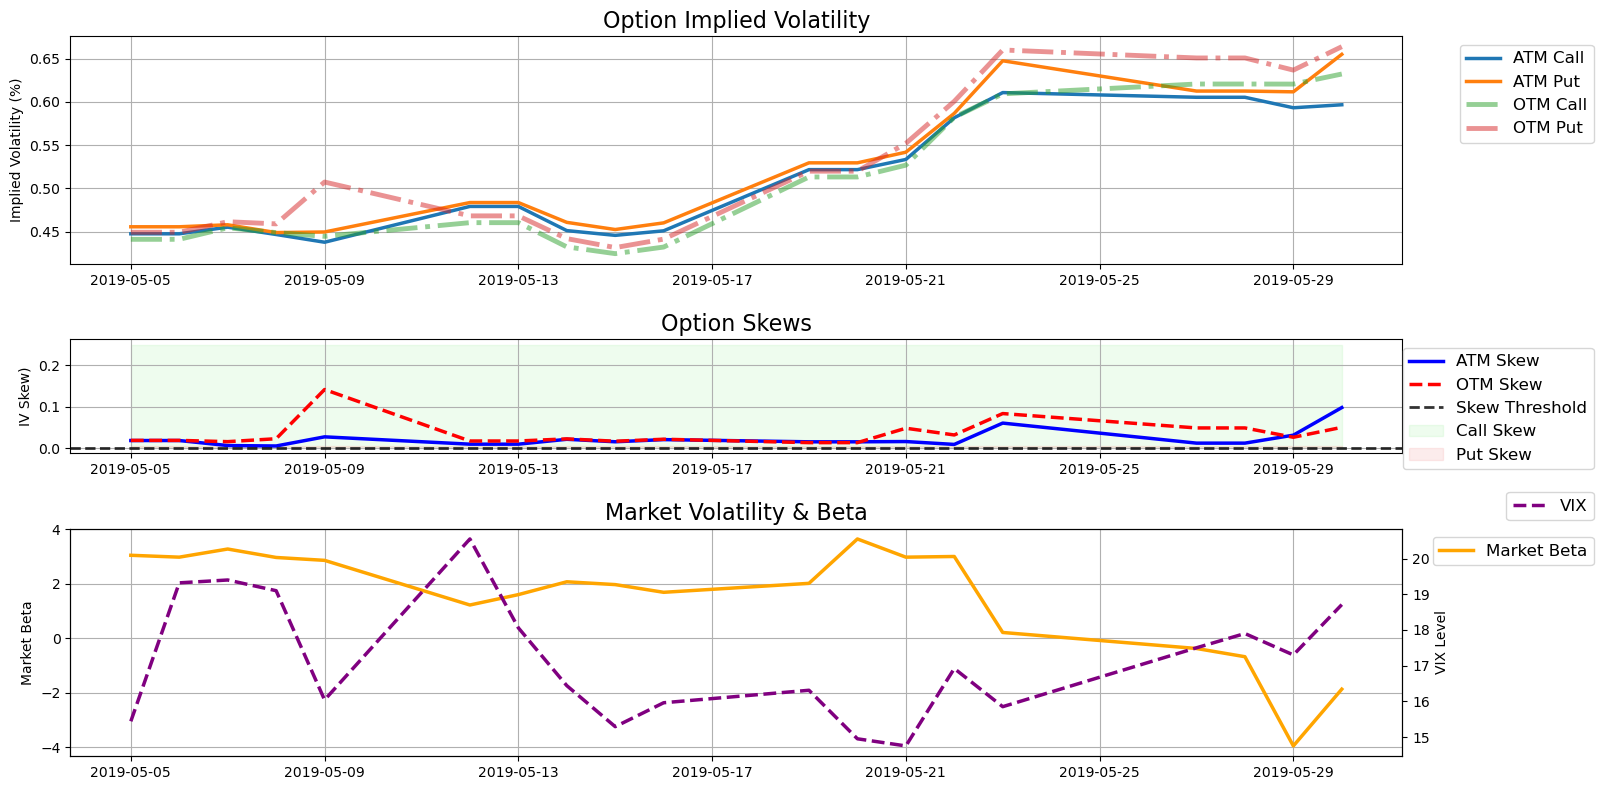
\includegraphics[width=1\linewidth]{judge_reviews/TSLA_M_gpt-4o-mini/2019-05-01/llm_Market_Volatility_&_Beta.png}
    \caption{Volatility after LLM's decision}
\end{figure}

\begin{tcolorbox}[colback=blue!10, colframe=blue!60, title=\textbf{TASKS}, sharp corners=southwest]
\begin{enumerate}
    \item Fill in the Expert Scoring \textit{rubric}.
    \item If applicable, provide \textit{examples} to correct the strategy.
\end{enumerate}
\end{tcolorbox}

\newpage


\section*{LLM Strategy 2}
\label{app:s2}

\subsection*{Historic 1 Year Data}

\begin{figure}[H]
    \centering
    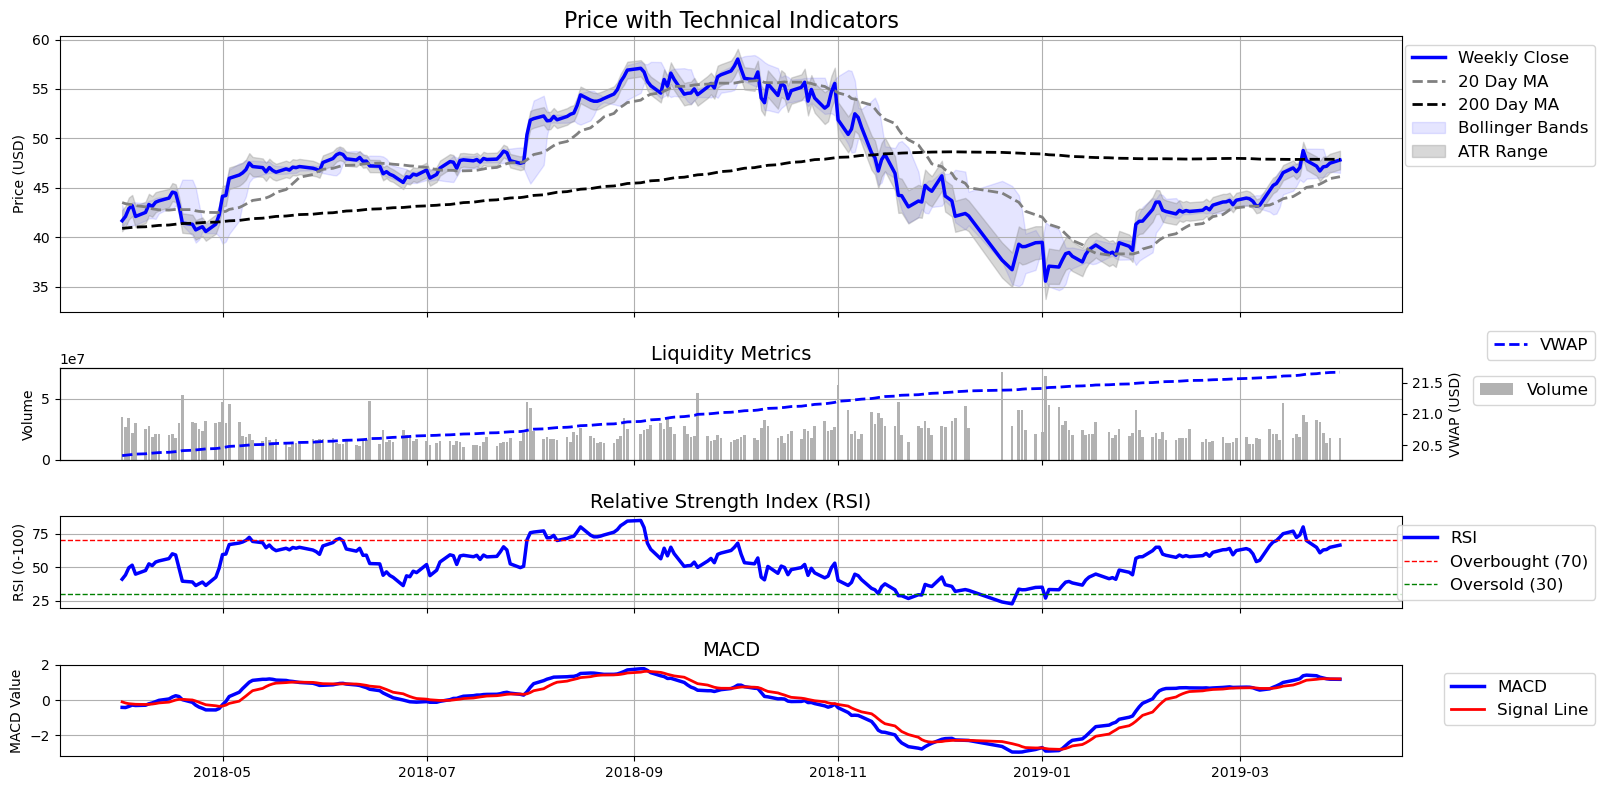
\includegraphics[width=1\linewidth]{judge_reviews/AAPL_M_gpt-4o-mini/2019-04-01/judge_Price_with_Technical_Indicators.png}
    \caption{Price and Technicals}
\end{figure}

\begin{figure}[H]
    \centering
    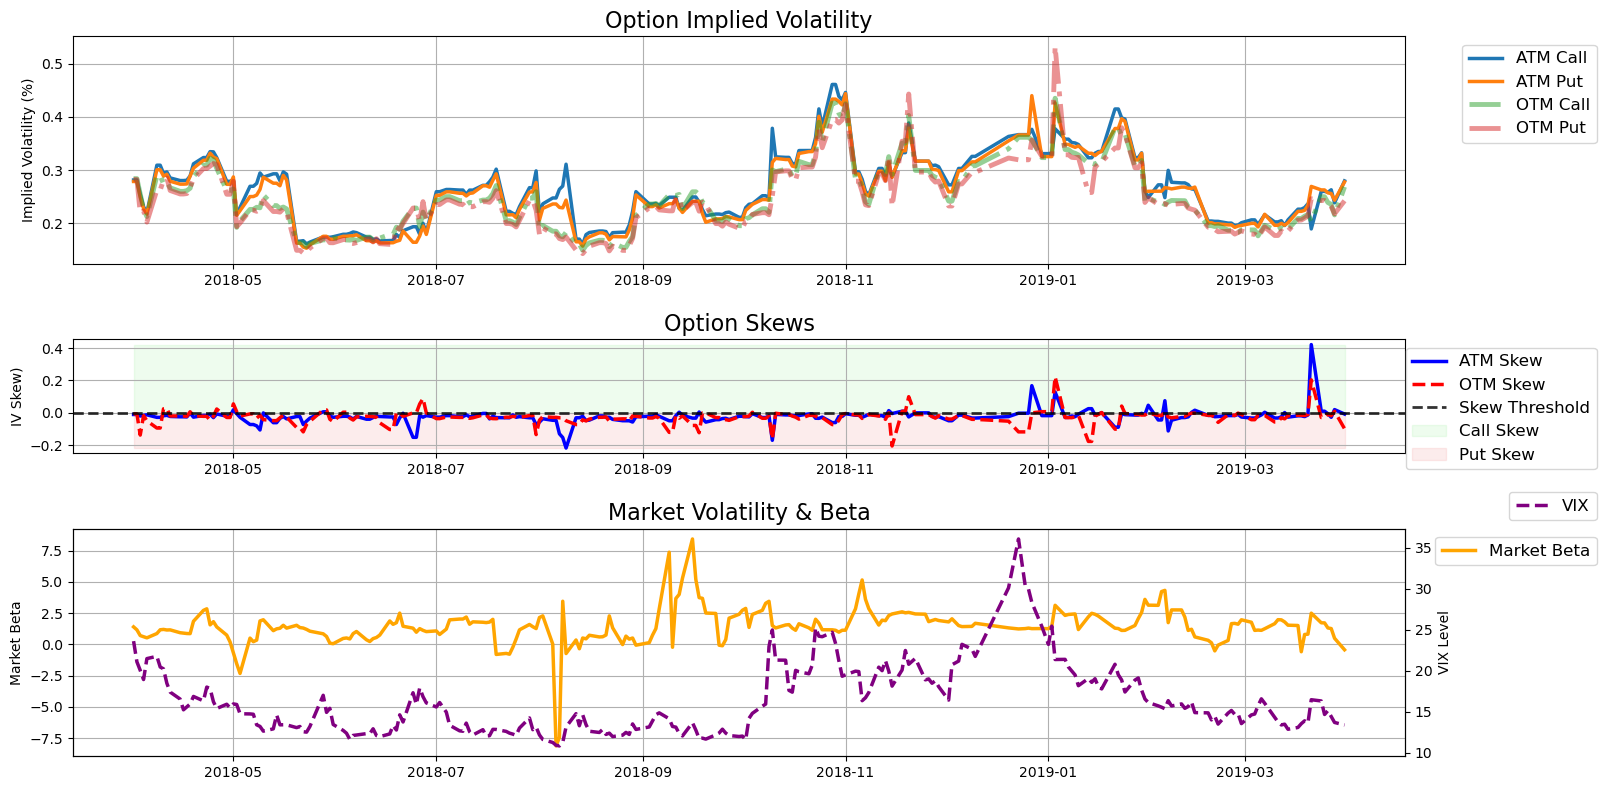
\includegraphics[width=1\linewidth]{judge_reviews/AAPL_M_gpt-4o-mini/2019-04-01/judge_Option_Implied_Volatility.png}
    \caption{Options}
\end{figure}

\begin{figure}[H]
    \centering
    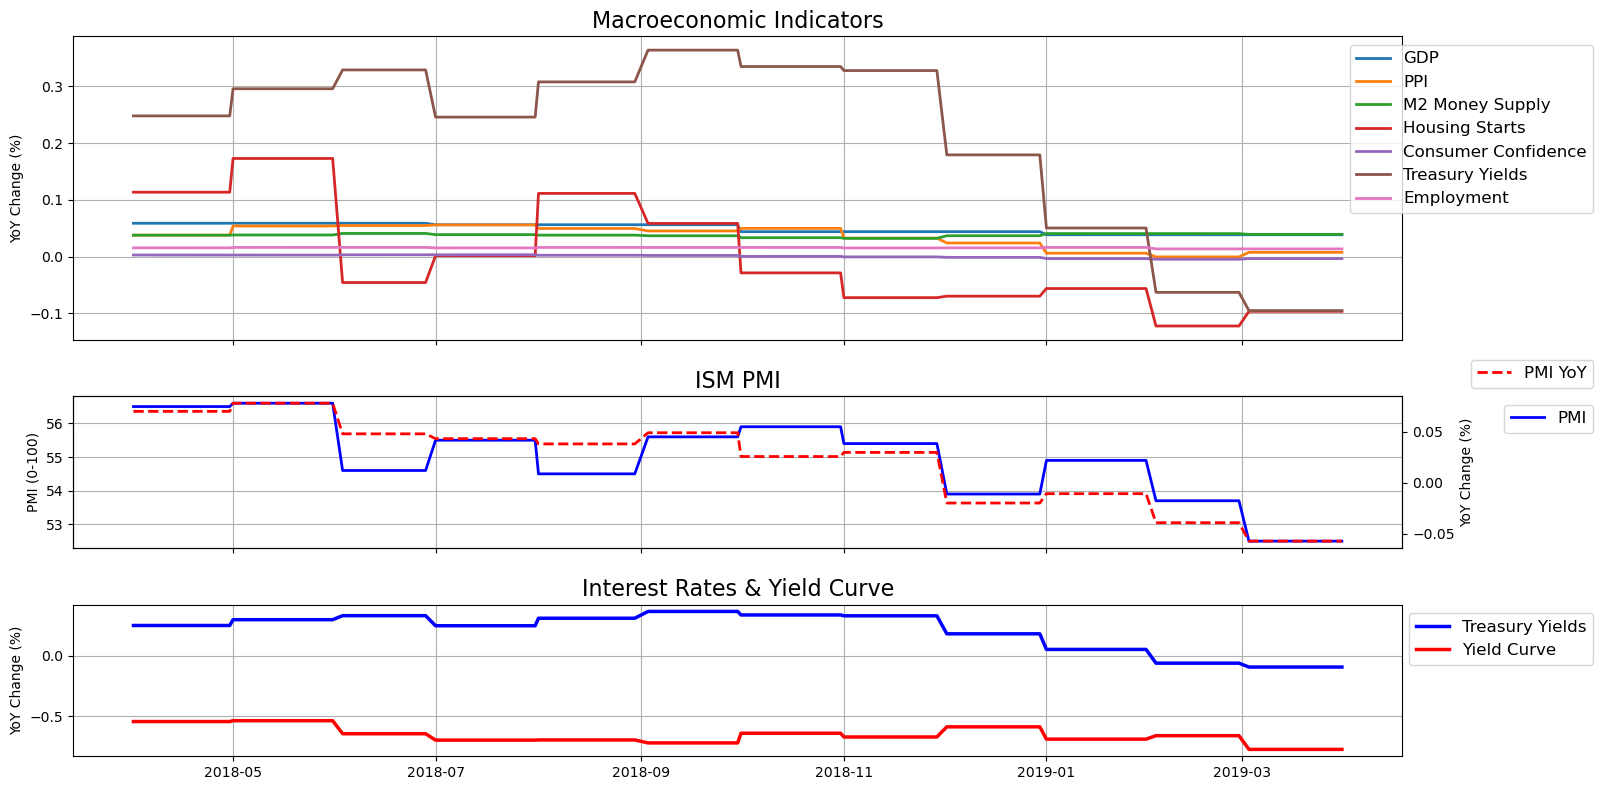
\includegraphics[width=1\linewidth]{judge_reviews/AAPL_M_gpt-4o-mini/2019-04-01/judge_Macroeconomic_Indicators.png}
    \caption{Macroeconomic}
\end{figure}

\begin{figure}[H]
    \centering
    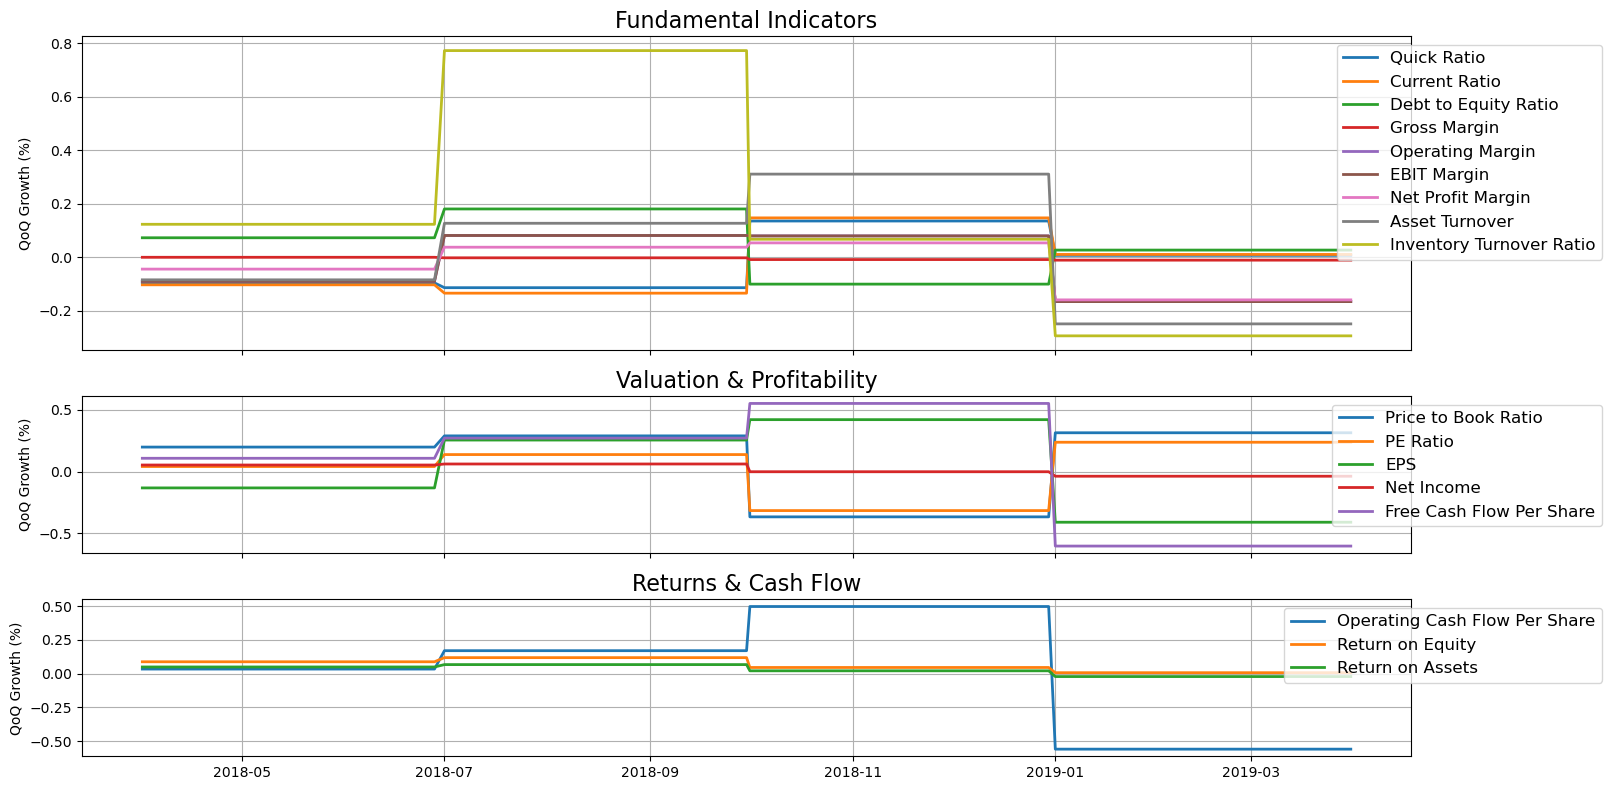
\includegraphics[width=1\linewidth]{judge_reviews/AAPL_M_gpt-4o-mini/2019-04-01/judge_Fundamental_Indicators.png}
    \caption{Fundamentals}
\end{figure}


\subsection*{Historic 1 Month News}

\textbf{Increased Regulatory Scrutiny on Tech Companies}
Amid growing concerns over data privacy and antitrust regulations, government agencies are considering imposing stricter oversight on major tech firms, including THE COMPANY. Analysts speculate that potential legal battles or regulatory fines could impact THE COMPANY’s ability to innovate freely and expand its services sector.

\textbf{Supply Chain Disruptions Affecting Production}
Recent reports highlight supply chain constraints affecting key components in THE COMPANY’s flagship product. Delays in procurement and rising material costs have forced THE COMPANY to adjust production schedules, raising concerns about meeting consumer demand in the upcoming quarters.

\textbf{Expansion of THE COMPANY’s Services Sector}
THE COMPANY is accelerating its push into subscription-based services, introducing new offerings aimed at diversifying revenue streams beyond hardware sales. Analysts view this as a strategic move to reduce dependency on product cycles and strengthen long-term financial stability.

\textbf{Legal Dispute Over Intellectual Property}
A recent legal battle involving THE COMPANY and a competitor over key patents in software and hardware integration has escalated. While THE COMPANY asserts its technology leadership, potential litigation outcomes could impact future product developments and licensing agreements.

\textbf{Market Reaction to Economic Indicators}
Recent economic data, including consumer spending trends and inflation reports, have influenced investor sentiment toward THE COMPANY. Market analysts are closely watching how macroeconomic conditions will affect THE COMPANY’s pricing strategy and global sales performance.

\begin{tcolorbox}[colback=blue!10, colframe=blue!60, title=\textbf{TASKS}, sharp corners=southwest]
\begin{enumerate}
    \item Guess the action to take: \textit{LONG} or \textit{SHORT}.
    \item Write a 1-2 sentence \textit{explanation} on why you decided the action above.
\end{enumerate}
\end{tcolorbox}

\textbf{NEXT PAGE}: Model's Decision and Rationale.

\newpage

\subsection*{LLMs' Strategy} \label{strategy2}

The traded instrument was AAPL, with the trading period set between 2019-04-07 and 2019-05-05.

\textbf{LLMs' decision: \textit{LONG}}

\textbf{Rationale}: The analysis indicates a bullish strategy for the next month based on several compelling factors. First, the stock's current close price of 44.05 is above both its 20MA (42.11) and 50MA (42.86), suggesting upward momentum (Feature: Stock\_Data.Price.Close). Second, with an RSI value of 58.26, it indicates that the stock is not overbought yet and may have room to run higher before reaching overbought conditions (Feature: Technical\_Analysis.RSI.Value). Third, despite recent volatility indicated by a historical volatility of approximately 27.78\%, the implied volatility at around 22.63\% suggests that options are priced favorably for potential upside moves (Feature: Implied\_Volatility.IV\_Close). Fourth, fundamental growth metrics such as EPS YoY at approximately 28\% signal strong earnings potential which supports price appreciation (Feature: Fundamental\_Data.Growth\_Metrics.EPS\_YoY). Lastly, news analysis reveals positive sentiment from market analysts regarding improved production capabilities; this aligns with pricing trends and reinforces confidence in future profitability due to reduced dependence on external suppliers.

\textbf{Top weighted features influencing this decision}:
\begin{enumerate}
    \item Stock\_Data.Price.Close (44.05)
    \item Technical\_Analysis.RSI.Value (58.26)
    \item Implied\_Volatility.IV\_Close (22.63\%)
    \item Fundamental\_Data.Growth\_Metrics.EPS\_YoY (28\%)
    \item Historical\_Volatility (27.78\%)
\end{enumerate}

\textbf{Key news impacting this strategy}:
\begin{enumerate}
    \item Market analysts upgraded ratings on THE COMPANY due to improved production capabilities - Market Impact Score: 4/5
    \item The strategic shift to self-manufactured chips potentially enhancing profit margins - Market Impact Score: 4/5
    \item Mixed sentiments about production targets indicating cautious optimism but manageable risk - Market Impact Score: 3/5
\end{enumerate}

\textbf{LLM Decision Insights}

\begin{longtable}{l c}
\toprule
\textbf{LLM Decision Insights} & \textbf{Value} \\
\midrule
Long Probability & 0.65 \\
Short Probability & 0.35 \\
Perplexity & 9.14316e+15 \\
\midrule
Total Tokens & 38845 \\
Total Cost (USD) & \$0.006040 \\
\bottomrule
\end{longtable}

\subsection*{Following Month Data}

\textbf{Performance Metrics}

\begin{longtable}{l c}
\toprule
\textbf{Metric} & \textbf{Value} \\
\midrule
Sharpe Ratio (Annualized SR) & 1.89417 \\
Portfolio Turnover (PTR) & 0 \\
Maximum Drawdown (MDD) & 0.0893178 \\
Mean Drawdown Duration (MDDur) & 5 \\
Cumulative Returns & 0.0484561 \\
\bottomrule
\end{longtable}


\begin{figure}[H]
    \centering
    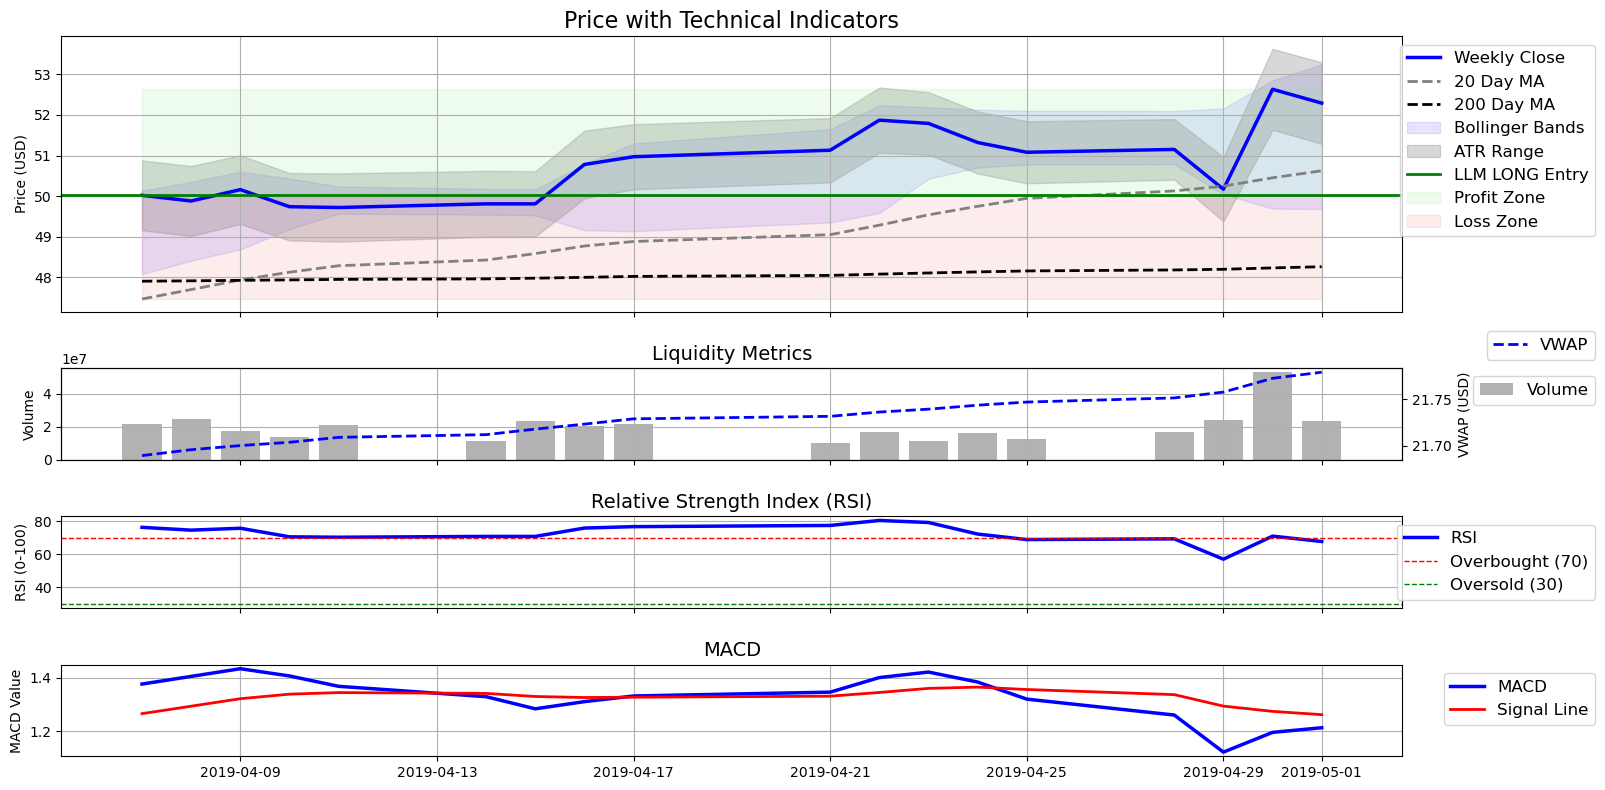
\includegraphics[width=1\linewidth]{judge_reviews//AAPL_M_gpt-4o-mini//2019-04-01/llm_Price_with_Technical_Indicators.png}
    \caption{Price after LLM's decision}
\end{figure}

\begin{figure}[H]
    \centering
    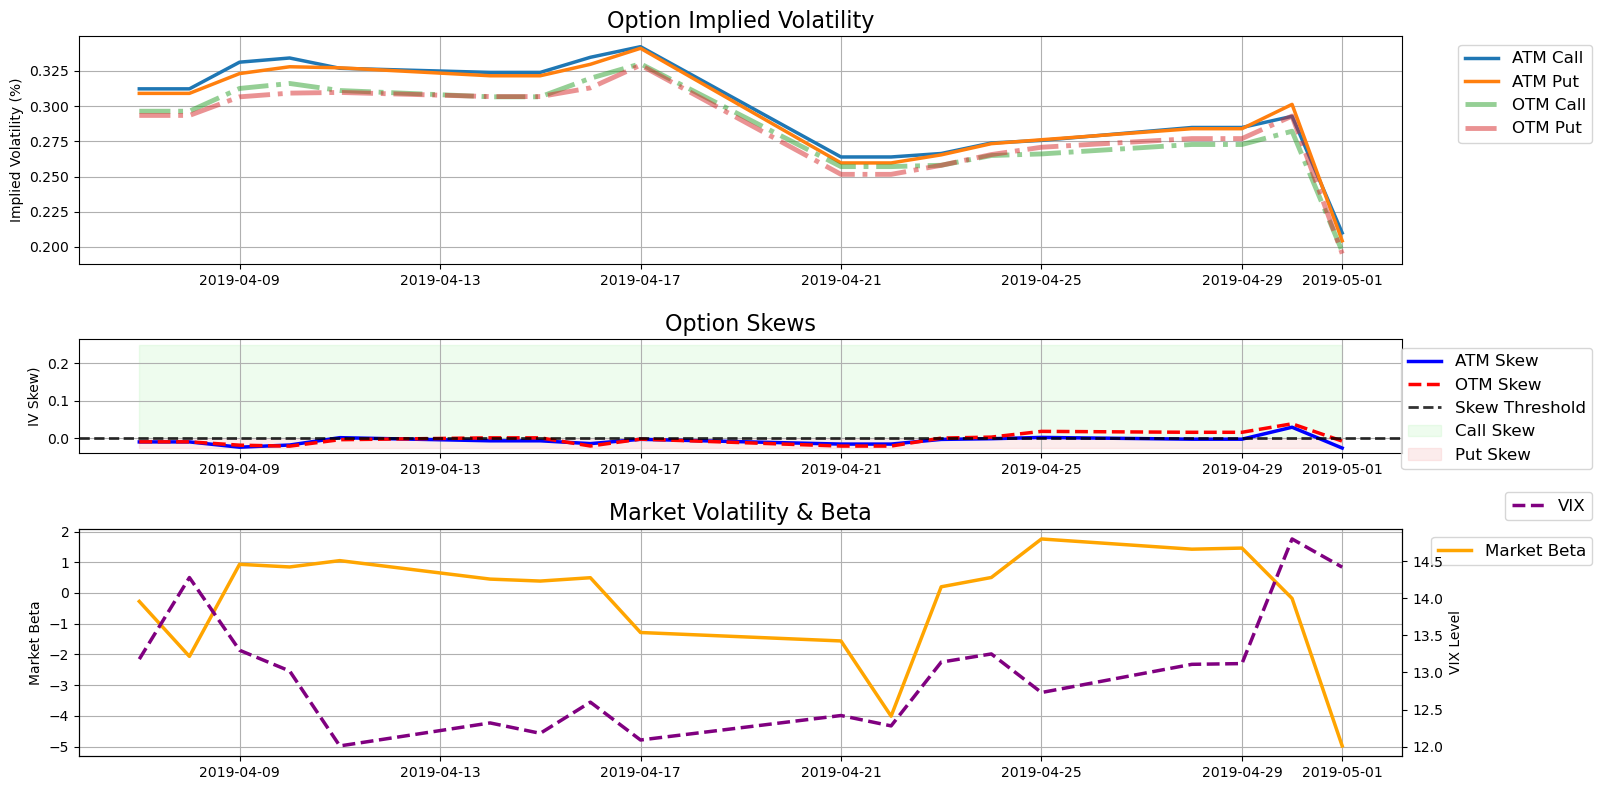
\includegraphics[width=1\linewidth]{judge_reviews/AAPL_M_gpt-4o-mini/2019-04-01/llm_Market_Volatility_&_Beta.png}
    \caption{Volatility after LLM's decision}
\end{figure}

\begin{tcolorbox}[colback=blue!10, colframe=blue!60, title=\textbf{TASKS}, sharp corners=southwest]
\begin{enumerate}
    \item Fill in the Expert Scoring \textit{rubric}.
    \item If applicable, provide \textit{examples} to correct the strategy.
\end{enumerate}
\end{tcolorbox}
\newpage


1\section*{LLM Strategy 3}
\label{app:s3}

\subsection*{Historic 1 Year Data}

\begin{figure}[H]
    \centering
    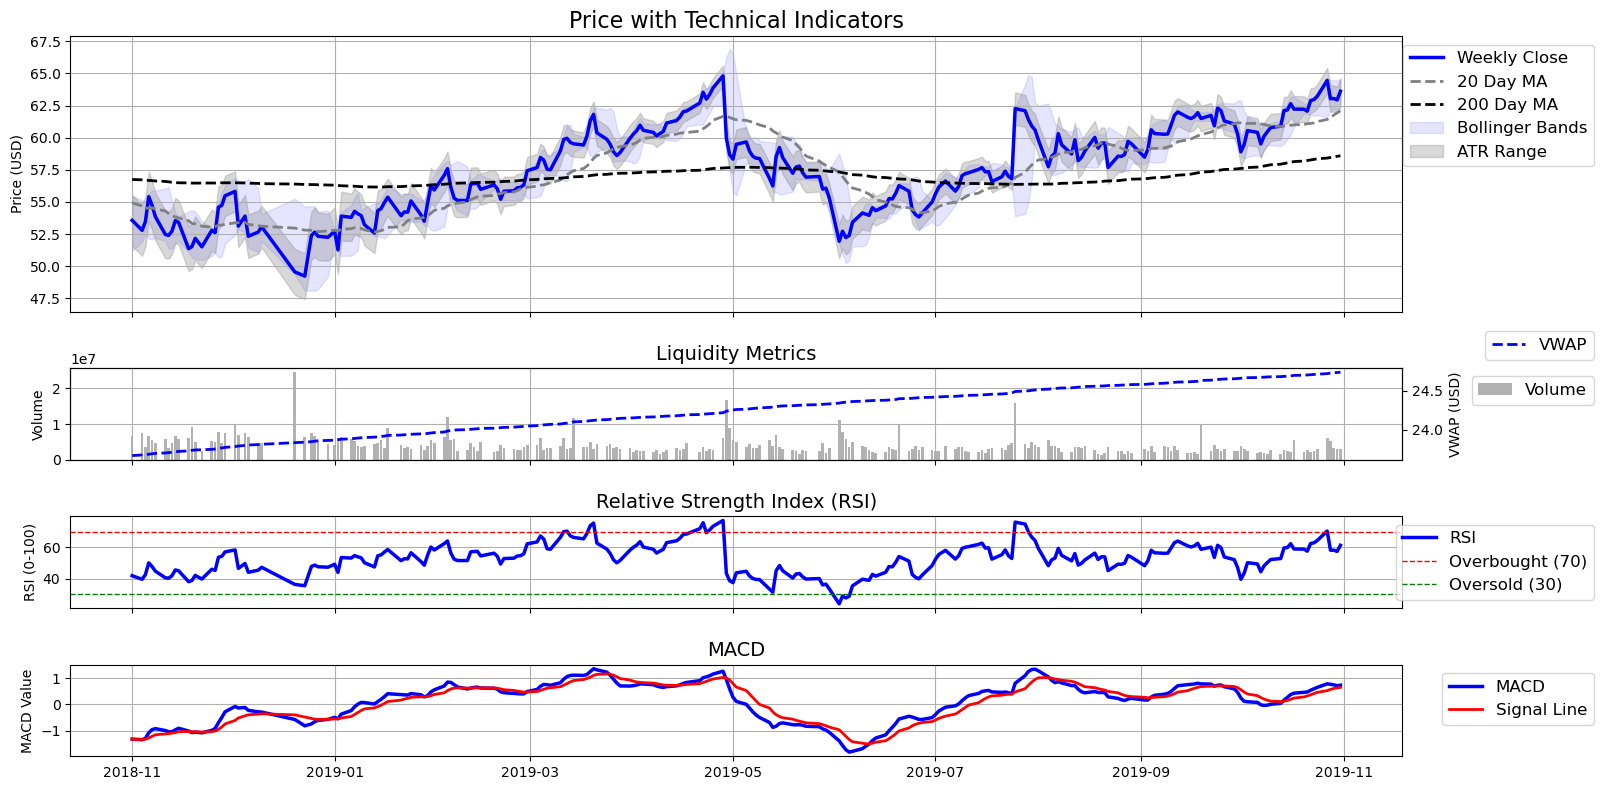
\includegraphics[width=1\linewidth]{judge_reviews//GOOGL_M_gpt-4o-mini//2019-11-01/judge_Price_with_Technical_Indicators.png}
    \caption{Price and Technicals}
\end{figure}

\begin{figure}[H]
    \centering
    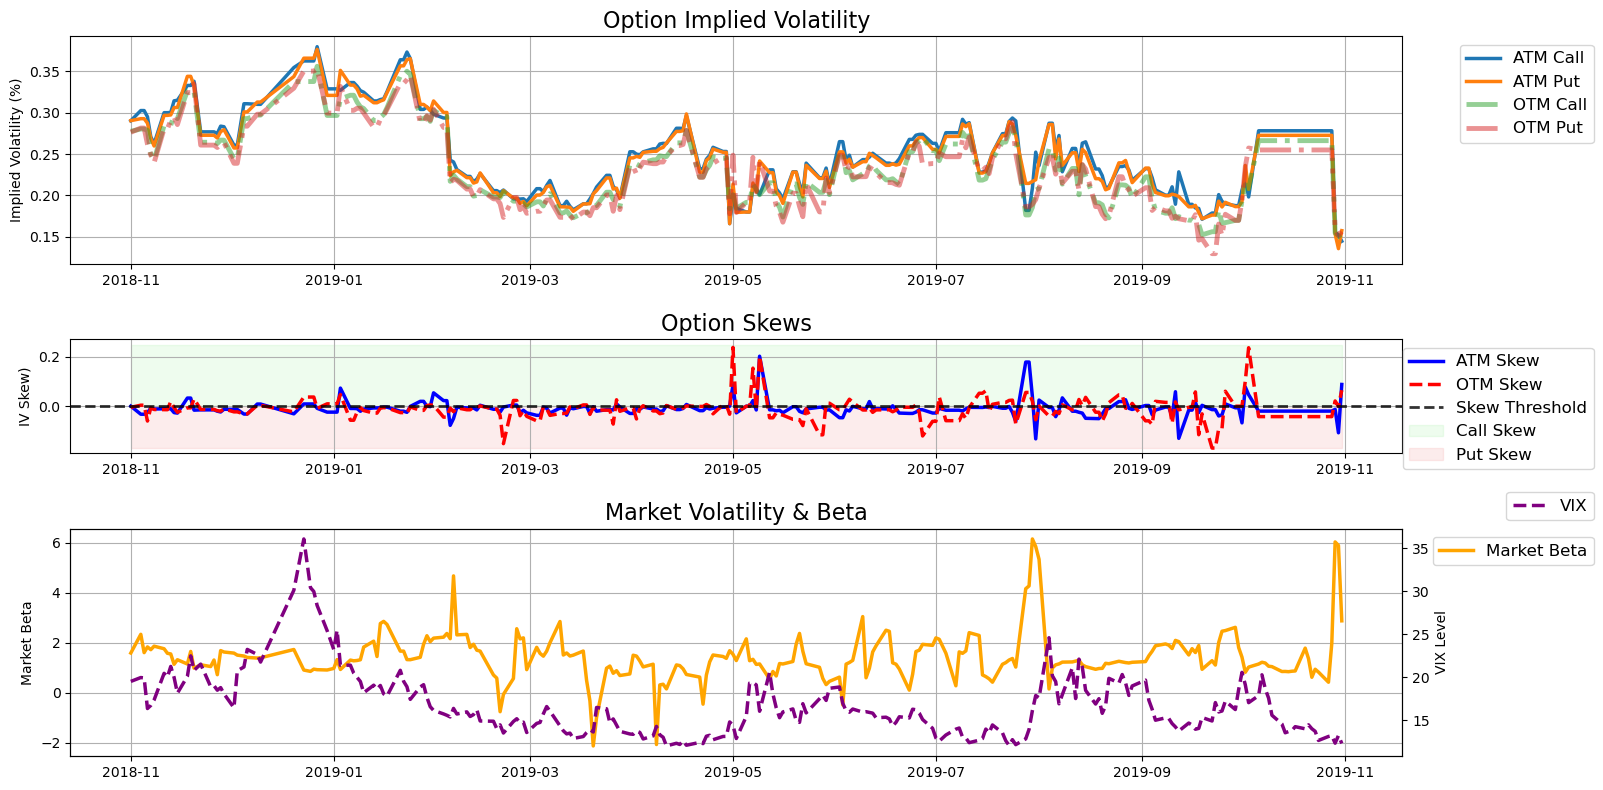
\includegraphics[width=1\linewidth]{judge_reviews/GOOGL_M_gpt-4o-mini/2019-11-01/judge_Option_Implied_Volatility.png}
    \caption{Options}
\end{figure}

\begin{figure}[H]
    \centering
    \includegraphics[width=1\linewidth]{judge_reviews/GOOGL_M_gpt-4o-mini/2019-11-01/judge_Macroeconomic_Indicators.png}
    \caption{Macroeconomic}
\end{figure}

\begin{figure}[H]
    \centering
    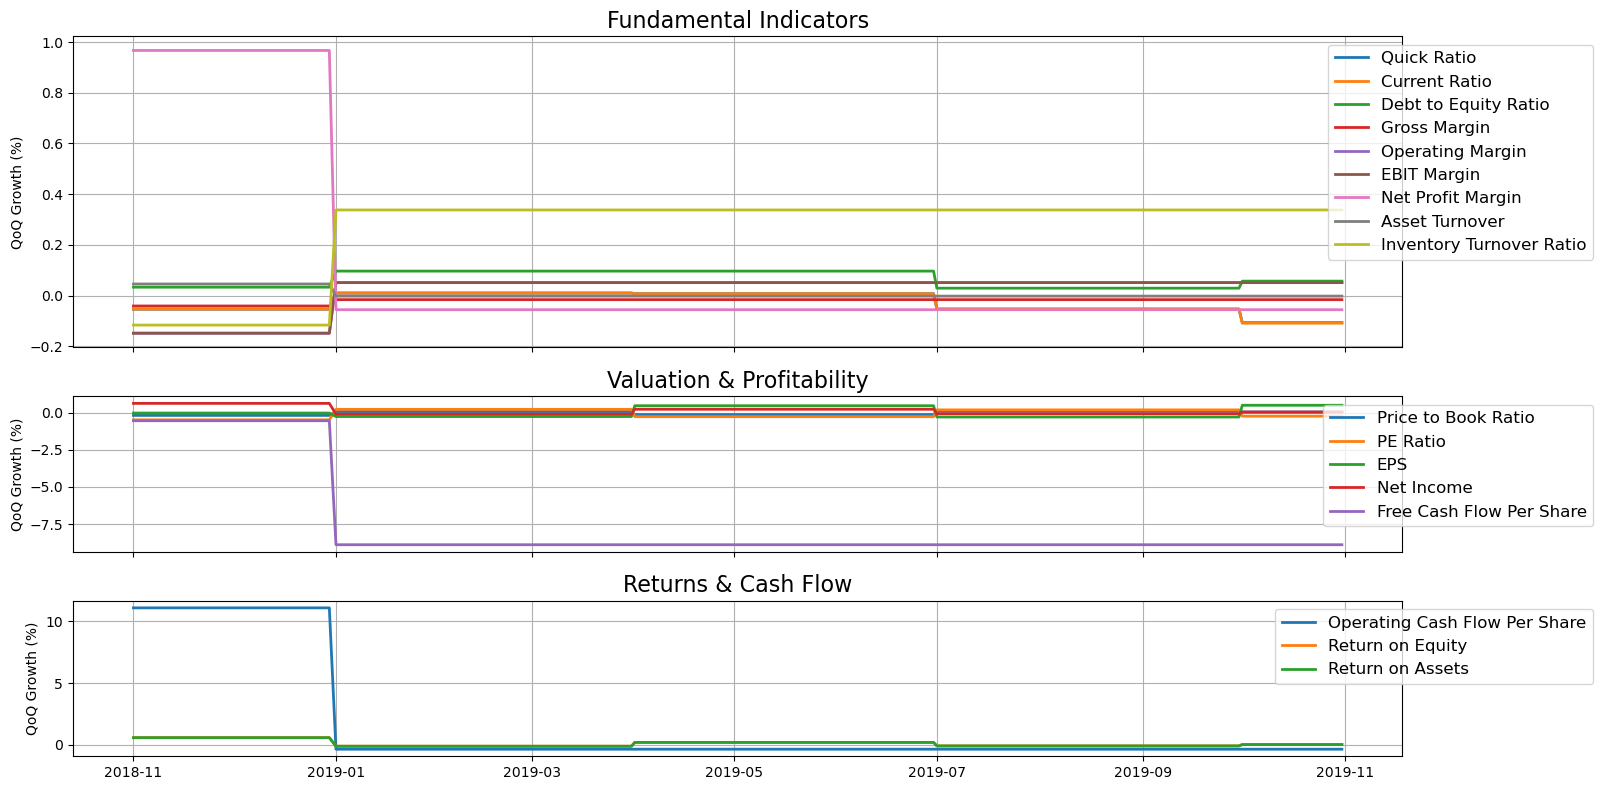
\includegraphics[width=1\linewidth]{judge_reviews/GOOGL_M_gpt-4o-mini/2019-11-01/judge_Fundamental_Indicators.png}
    \caption{Fundamentals}
\end{figure}

\subsection*{Historic 1 Month News}

\textbf{Regulatory Scrutiny on Data Privacy}
THE COMPANY is facing increased regulatory attention over data privacy concerns. Lawmakers are considering stricter policies that could impact THE COMPANY’s advertising and services revenue. Investors are closely watching potential changes that might affect business operations and user engagement.

\textbf{Supply Chain Disruptions and Production Adjustments}
Reports indicate that THE COMPANY is experiencing supply chain constraints, leading to adjustments in production targets. While THE COMPANY is working to mitigate these issues through alternative sourcing strategies, analysts are concerned about potential delays in delivering key products to market.

\textbf{Expansion into Subscription-Based Services}
THE COMPANY is accelerating its transition into subscription-based services, introducing new offerings that aim to reduce dependence on hardware sales. Analysts view this as a strategic move that could provide more consistent revenue streams amid fluctuating device sales.

\textbf{Legal Disputes Over Patents and Licensing}
A legal dispute has emerged between THE COMPANY and a competitor over intellectual property related to software and hardware integration. The outcome of this case could have long-term implications for THE COMPANY’s innovation strategy and licensing agreements.

\textbf{Macroeconomic Factors Impacting Market Performance}
Recent economic indicators, including inflation and consumer spending trends, have influenced investor sentiment toward THE COMPANY. Analysts are evaluating how broader market conditions could affect THE COMPANY’s pricing strategies and overall demand for its products.


\begin{tcolorbox}[colback=blue!10, colframe=blue!60, title=\textbf{TASKS}, sharp corners=southwest]
\begin{enumerate}
    \item Guess the action to take: \textit{LONG} or \textit{SHORT}.
    \item Write a 1-2 sentence \textit{explanation} on why you decided the action above.
\end{enumerate}
\end{tcolorbox}
\textbf{NEXT PAGE}: Model's Decision and Rationale.

\newpage

\subsection*{LLMs' Strategy} \label{strategy3}

The traded instrument was GOOGL, with the trading period set between 2019-11-04 and 2019-12-02.

\textbf{LLMs' decision: \textit{LONG}}

\textbf{Rationale}: The current analysis indicates a positive outlook for the stock based on several key factors. Firstly, the stock is trading above its 20-day moving average (61.15) and shows strong weekly past returns (1.66\%, 1.23\%, 2.19\%, 0.24\%), suggesting bullish momentum despite recent price dips below the MA levels, particularly influenced by external competition pressures.

Secondly, while the RSI value is at 39.67 indicating it's approaching oversold territory, this suggests potential for a rebound which aligns with recent analyst upgrades and positive earnings projections that hint at strong future demand in an evolving EV market.

Thirdly, macroeconomic indicators such as GDP growth (0.0099) and PMI (51.1), along with declining Treasury yields (-0.457), suggest a risk-on environment favorable for high-growth tech stocks like ours.

Fourthly, news factors also play a crucial role: "Analysts predict significant rebounds in deliveries," score of **4 out of 5**; "Strategic collaboration expected to enhance product offerings," score of **5 out of 5**; and "Analyst upgrades suggest bullish outlook," score of **4 out of 5**, all indicate strong market confidence.

Lastly, considering the implied volatility skews are stable relative to historical volatility levels supports taking on positions anticipating upward movement as investor sentiment improves post-competition announcements.

\textbf{Top weighted features influencing this decision}:
\begin{enumerate}
    \item Stock\_Data.Price.Close (61.15)
    \item Technical\_Analysis.RSI.Value (39.67)
    \item Macro\_Indicators.GDP\_QoQ (0.0099)
    \item Macro\_Indicators.PMI (51.1)
    \item Implied\_Volatility.IV\_Close (-0.457)
\end{enumerate}

\textbf{Key news impacting this strategy}:
\begin{enumerate}
    \item Analysts predict significant rebounds in deliveries - Market Impact Score: 4/5
    \item Strategic collaboration expected to enhance product offerings - Market Impact Score: 5/5
    \item Analyst upgrades suggest bullish outlook - Market Impact Score: 4/5
\end{enumerate}

\textbf{LLM Decision Insights}

\begin{longtable}{l c}
\toprule
\textbf{LLM Decision Insights} & \textbf{Value} \\
\midrule
Long Probability & 0.75 \\
Short Probability & 0.25 \\
Perplexity & 5.36689e+29 \\
\midrule
Total Tokens & 21817 \\
Total Cost (USD) & \$0.003487 \\
\bottomrule
\end{longtable}

\subsection*{Following Month Data}

\textbf{Performance Metrics}

\begin{longtable}{l c}
\toprule
\textbf{Metric} & \textbf{Value} \\
\midrule
Sharpe Ratio (Annualized SR) & -0.299606 \\
Portfolio Turnover (PTR) & 0 \\
Maximum Drawdown (MDD) & 0.0335933 \\
Mean Drawdown Duration (MDDur) & 4.42857 \\
Cumulative Returns & -0.00201332 \\
\bottomrule
\end{longtable}

\begin{figure}[H]
    \centering
    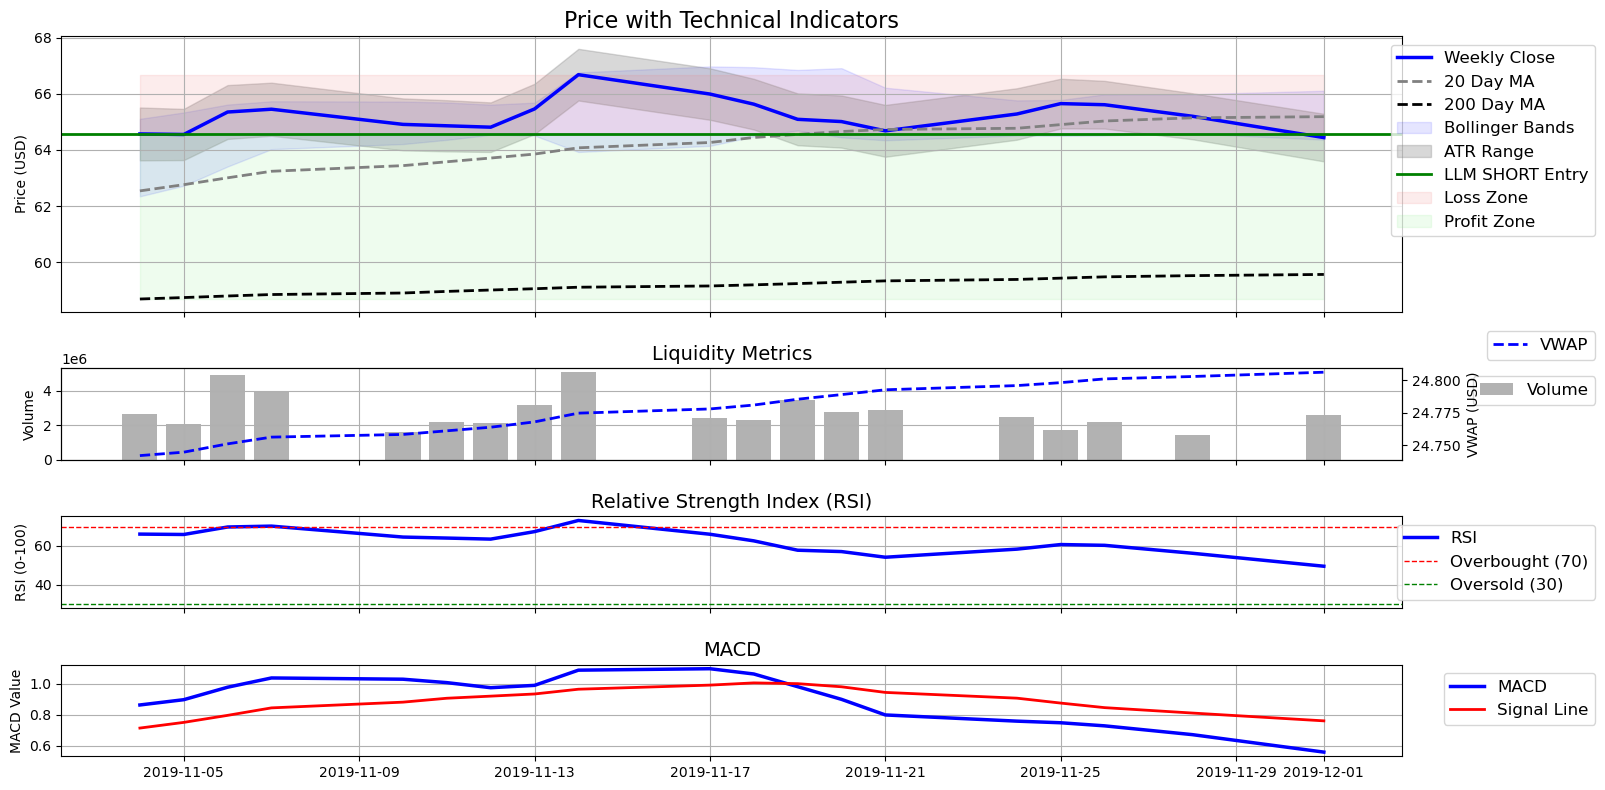
\includegraphics[width=1\linewidth]{judge_reviews//GOOGL_M_gpt-4o-mini//2019-11-01/llm_Price_with_Technical_Indicators.png}
    \caption{Price after LLM's decision}
\end{figure}

\begin{figure}[H]
    \centering
    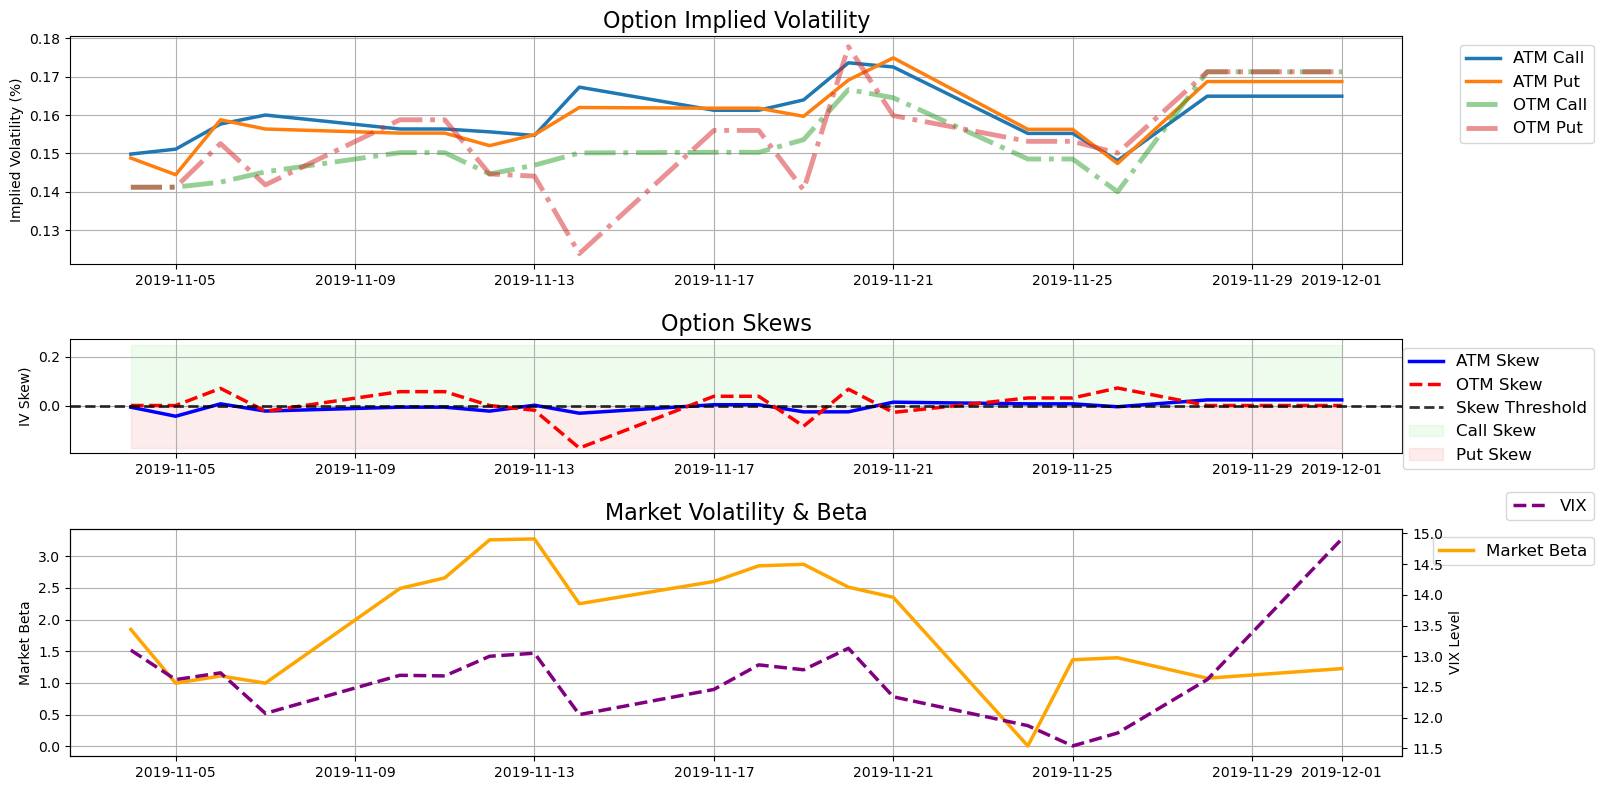
\includegraphics[width=1\linewidth]{judge_reviews/GOOGL_M_gpt-4o-mini/2019-11-01/llm_Market_Volatility_&_Beta.png}
    \caption{Volatility after LLM's decision}
\end{figure}

\begin{tcolorbox}[colback=blue!10, colframe=blue!60, title=\textbf{TASKS}, sharp corners=southwest]
\begin{enumerate}
    \item Fill in the Expert Scoring \textit{rubric}.
    \item If applicable, provide \textit{examples} to correct the strategy.
\end{enumerate}
\end{tcolorbox}
\newpage


\section*{LLM Strategy 4}
\label{app:s4}

\subsection*{Historic 1 Year Data}

\begin{figure}[H]
    \centering
    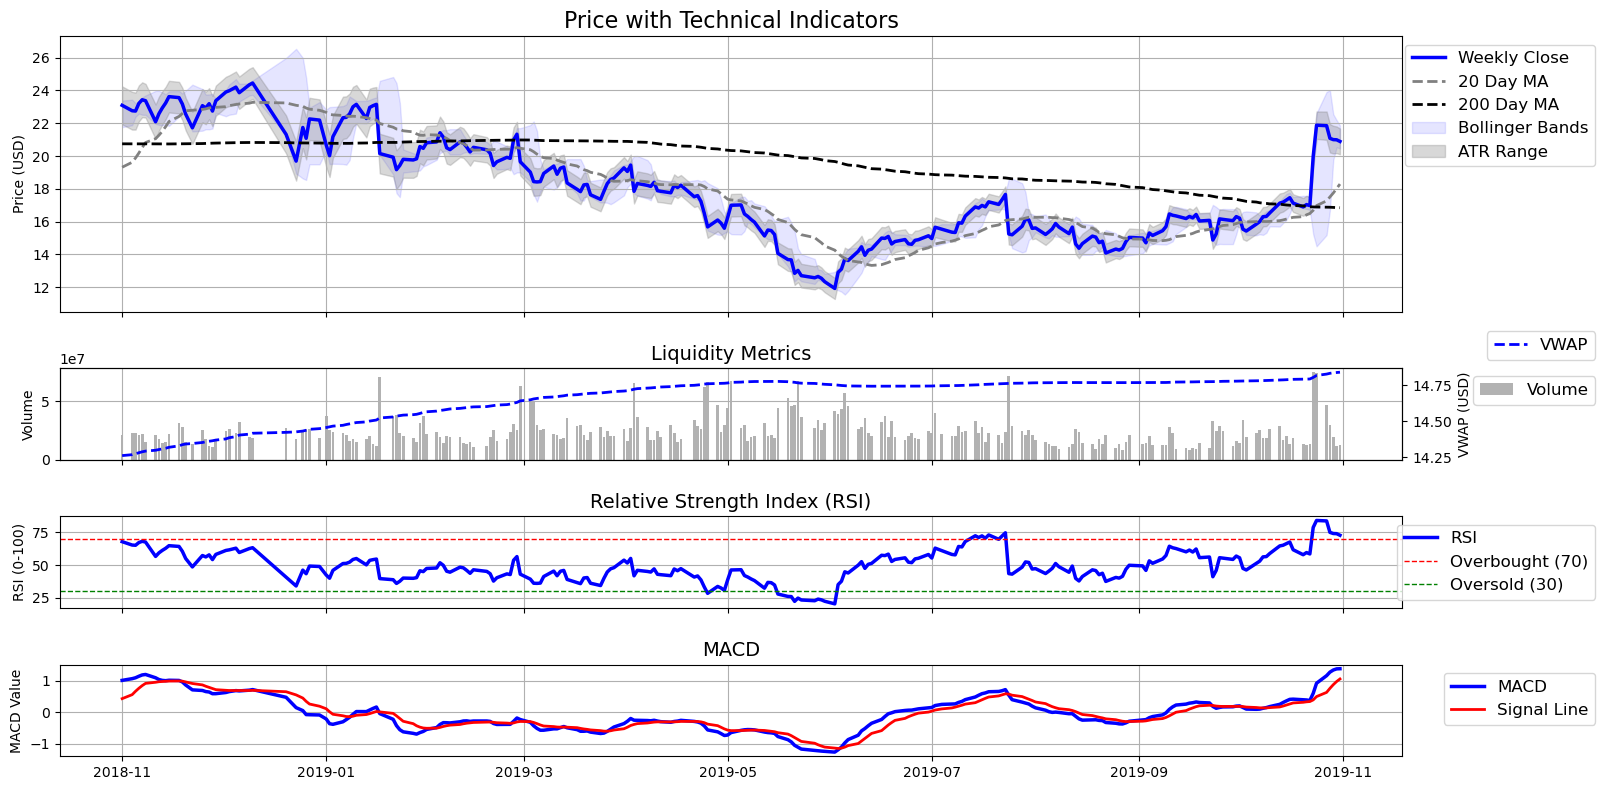
\includegraphics[width=1\linewidth]{judge_reviews//TSLA_M_gpt-4o-mini//2019-11-01/judge_Price_with_Technical_Indicators.png}
    \caption{Price and Technicals}
\end{figure}

\begin{figure}[H]
    \centering
    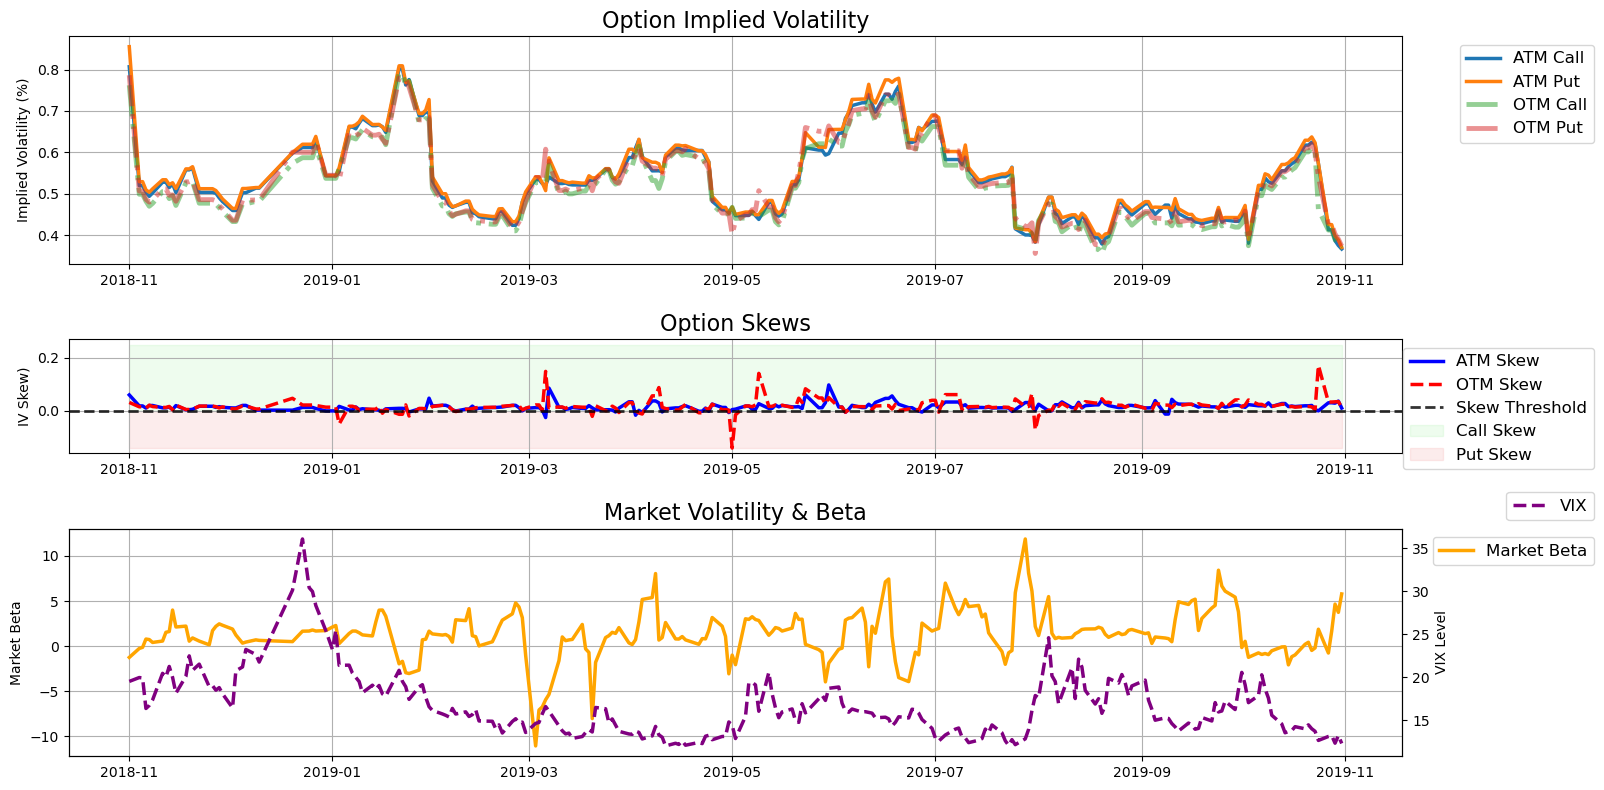
\includegraphics[width=1\linewidth]{judge_reviews/TSLA_M_gpt-4o-mini/2019-11-01/judge_Option_Implied_Volatility.png}
    \caption{Options}
\end{figure}

\begin{figure}[H]
    \centering
    \includegraphics[width=1\linewidth]{judge_reviews/TSLA_M_gpt-4o-mini/2019-11-01/judge_Macroeconomic_Indicators.png}
    \caption{Macroeconomic}
\end{figure}

\begin{figure}[H]
    \centering
    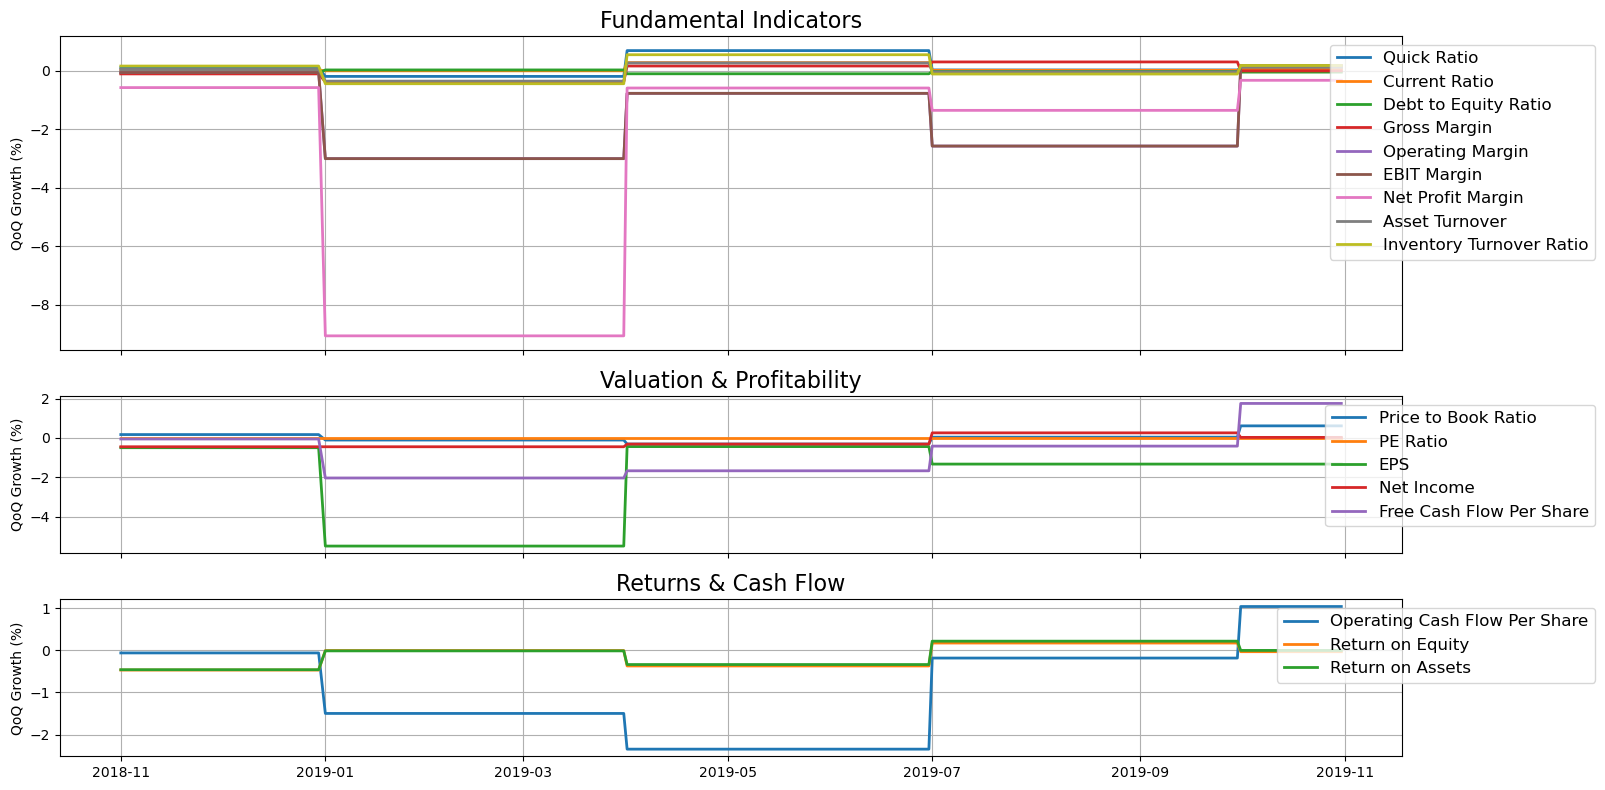
\includegraphics[width=1\linewidth]{judge_reviews/TSLA_M_gpt-4o-mini/2019-11-01/judge_Fundamental_Indicators.png}
    \caption{Fundamentals}
\end{figure}

\subsection*{Historic 1 Month News}

\textbf{Earnings Report Surpasses Expectations}
THE COMPANY reported earnings significantly above market expectations, with stronger-than-anticipated revenue and profitability. Analysts had projected a loss, but THE COMPANY's financials demonstrated resilience, driven by improved operational efficiency and cost management.

\textbf{Strategic Partnership to Enhance Product Offerings}
THE COMPANY announced a strategic collaboration with a major technology firm to enhance its next-generation product capabilities. This move is expected to improve market competitiveness and expand offerings, reinforcing its position in the industry.

\textbf{Market Confidence Boosted by Analyst Upgrades}
Several analysts revised their ratings upward for THE COMPANY, citing strong future growth prospects and improving financial stability. Investor sentiment turned more positive following these upgrades, leading to increased stock momentum.

\textbf{Macroeconomic Factors Favoring THE COMPANY}
Economic indicators, including GDP growth and declining treasury yields, have contributed to a favorable market environment for THE COMPANY. These factors have led to increased investor confidence in high-growth stocks, benefiting THE COMPANY’s valuation.

\textbf{Competitive Market Pressures Intensify}
A major competitor introduced a new product line, intensifying competition within the sector. While this development poses challenges, THE COMPANY's recent strategic initiatives and product advancements are expected to mitigate the competitive impact.


\begin{tcolorbox}[colback=blue!10, colframe=blue!60, title=\textbf{TASKS}, sharp corners=southwest]
\begin{enumerate}
    \item Guess the action to take: \textit{LONG} or \textit{SHORT}.
    \item Write a 1-2 sentence \textit{explanation} on why you decided the action above.
\end{enumerate}
\end{tcolorbox}
\textbf{NEXT PAGE}: Model's Decision and Rationale.

\newpage

\subsection*{LLMs' Strategy} \label{strategy4}

The traded instrument was TSLA, with the trading period set between 2019-11-04 and 2019-12-02.

\textbf{LLMs' decision: \textit{LONG}}

\textbf{Rationale}: The decision to pursue a LONG strategy is supported by multiple factors indicating bullish momentum and favorable market conditions. Key features include:
\begin{enumerate}
    \item \textbf{Stock\_Data.Price.Close}: The current price of 16.21 is above the 20MA (15.96) and the 50MA (15.50), suggesting positive momentum.
    \item \textbf{Technical\_Analysis.RSI.Value}: With an RSI of 55, the stock indicates potential for further upside as it approaches overbought territory (>70).
    \item \textbf{Options\_Data.Atm\_IV\_Skews}: The ATM IV skew shows stability, which coupled with high implied volatility suggests readiness to capitalize on upward price movement.
    \item \textbf{Growth Metrics (EPS YoY)}: Although EPS YoY is negative at -16\%, recent news suggests expected recovery due to new product demand and operational efficiencies from new facilities.
    \item \textbf{Macro\_Data.SPX.Close\_Slope}: The SPX close slope indicates a slight bearish trend; however, VIX trends are showing reduced fear in the market, supporting risk-on behavior.
\end{enumerate}

\textbf{Key news impacting this strategy}:
\begin{enumerate}
    \item Positive delivery statistics reported by THE COMPANY indicate a rebound in sales - Market Impact Score: 5/5
    \item Analysts raise price targets citing anticipated revenue growth - Market Impact Score: 4/5
    \item THE COMPANY announces plans for a new Gigafactory in Berlin, enhancing production efficiency - Market Impact Score: 4/5
\end{enumerate}

\textbf{LLM Decision Insights}

\begin{longtable}{l c}
\toprule
\textbf{LLM Decision Insights} & \textbf{Value} \\
\midrule
Long Probability & 0.75 \\
Short Probability & 0.25 \\
Perplexity & 8.61386e+12 \\
\midrule
Total Tokens & 21937 \\
Total Cost (USD) & \$0.003532 \\
\bottomrule
\end{longtable}

\subsection*{Following Month Data}

\textbf{Performance Metrics}

\begin{longtable}{l c}
\toprule
\textbf{Metric} & \textbf{Value} \\
\midrule
Sharpe Ratio (Annualized SR) & 2.18892 \\
Portfolio Turnover (PTR) & 0 \\
Maximum Drawdown (MDD) & 0.0851064 \\
Mean Drawdown Duration (MDDur) & 3.63636 \\
Cumulative Returns & 0.0553191 \\
\bottomrule
\end{longtable}

\begin{figure}[H]
    \centering
    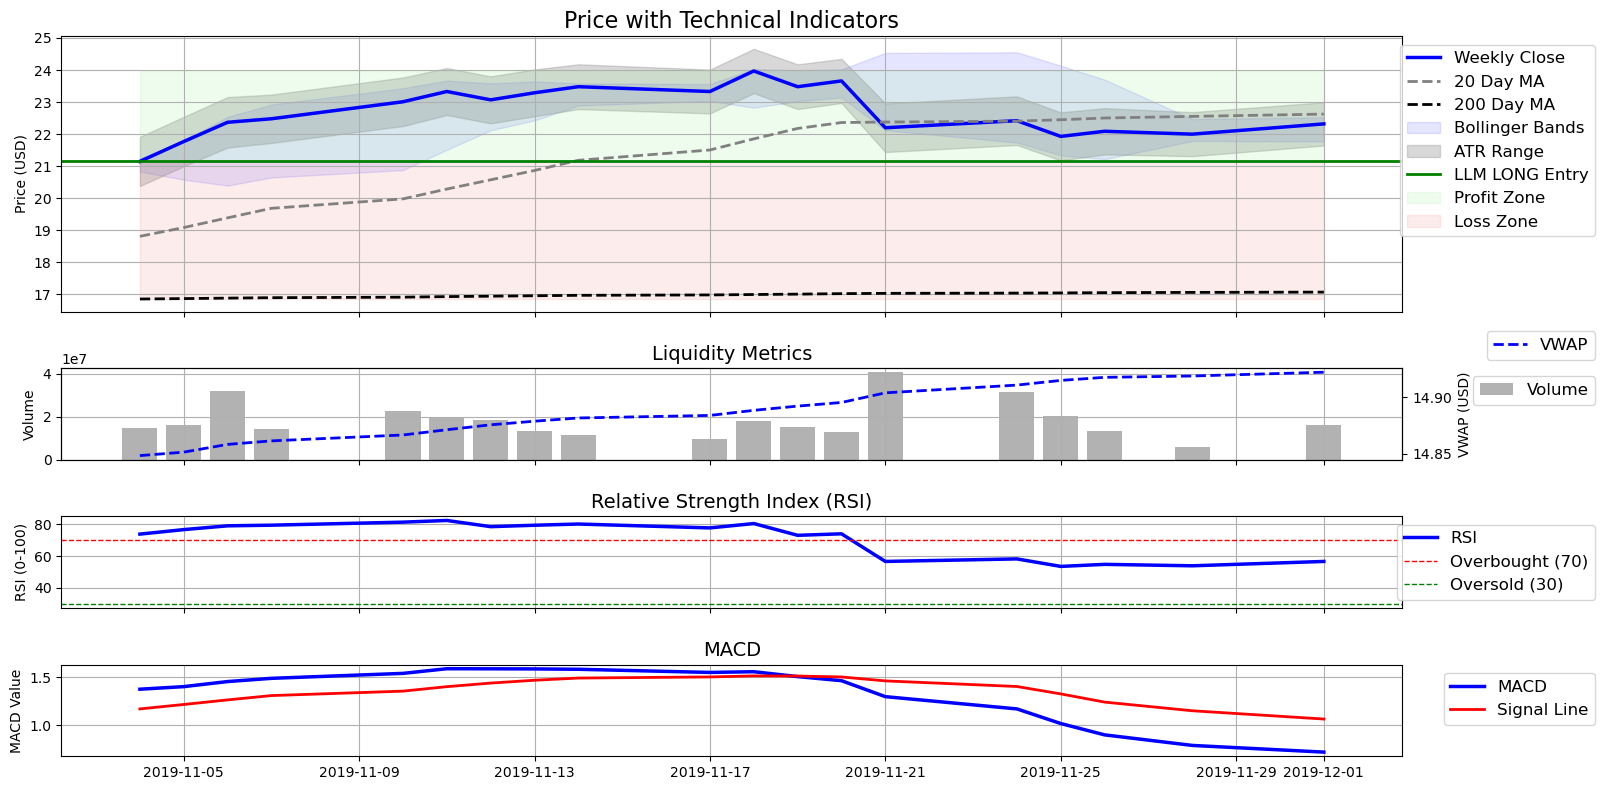
\includegraphics[width=1\linewidth]{judge_reviews//TSLA_M_gpt-4o-mini//2019-11-01/llm_Price_with_Technical_Indicators.png}
    \caption{Price after LLM's decision}
\end{figure}

\begin{figure}[H]
    \centering
    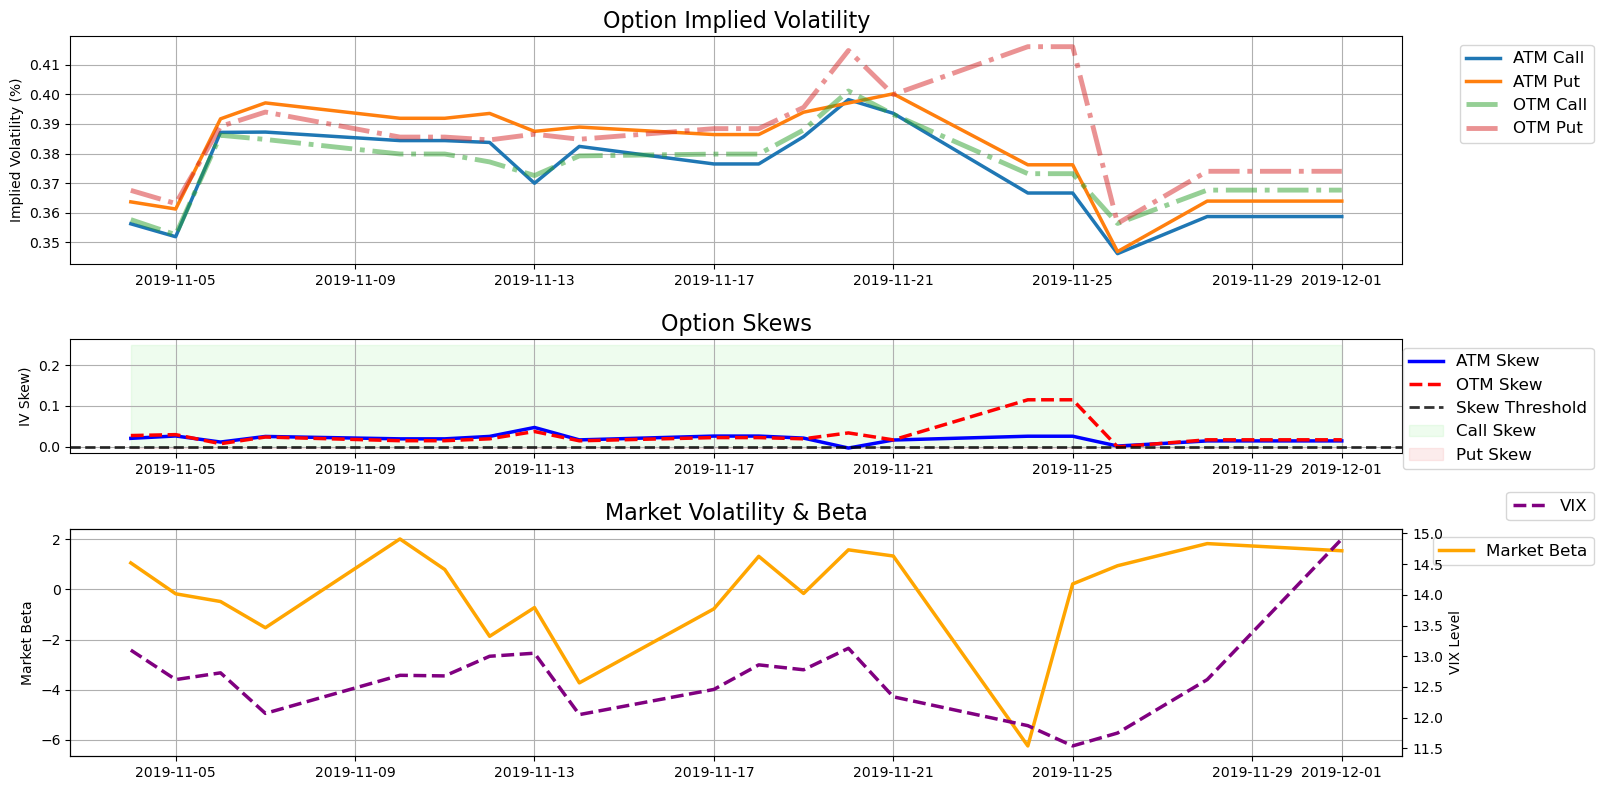
\includegraphics[width=1\linewidth]{judge_reviews/TSLA_M_gpt-4o-mini/2019-11-01/llm_Market_Volatility_&_Beta.png}
    \caption{Volatility after LLM's decision}
\end{figure}

\begin{tcolorbox}[colback=blue!10, colframe=blue!60, title=\textbf{TASKS}, sharp corners=southwest]
\begin{enumerate}
    \item Fill in the Expert Scoring \textit{rubric}.
    \item If applicable, provide \textit{examples} to correct the strategy.
\end{enumerate}
\end{tcolorbox}
\newpage


\section*{LLM Strategy 5}
\label{app:s5}

\subsection*{Historic 1 Year Data}

\begin{figure}[H]
    \centering
    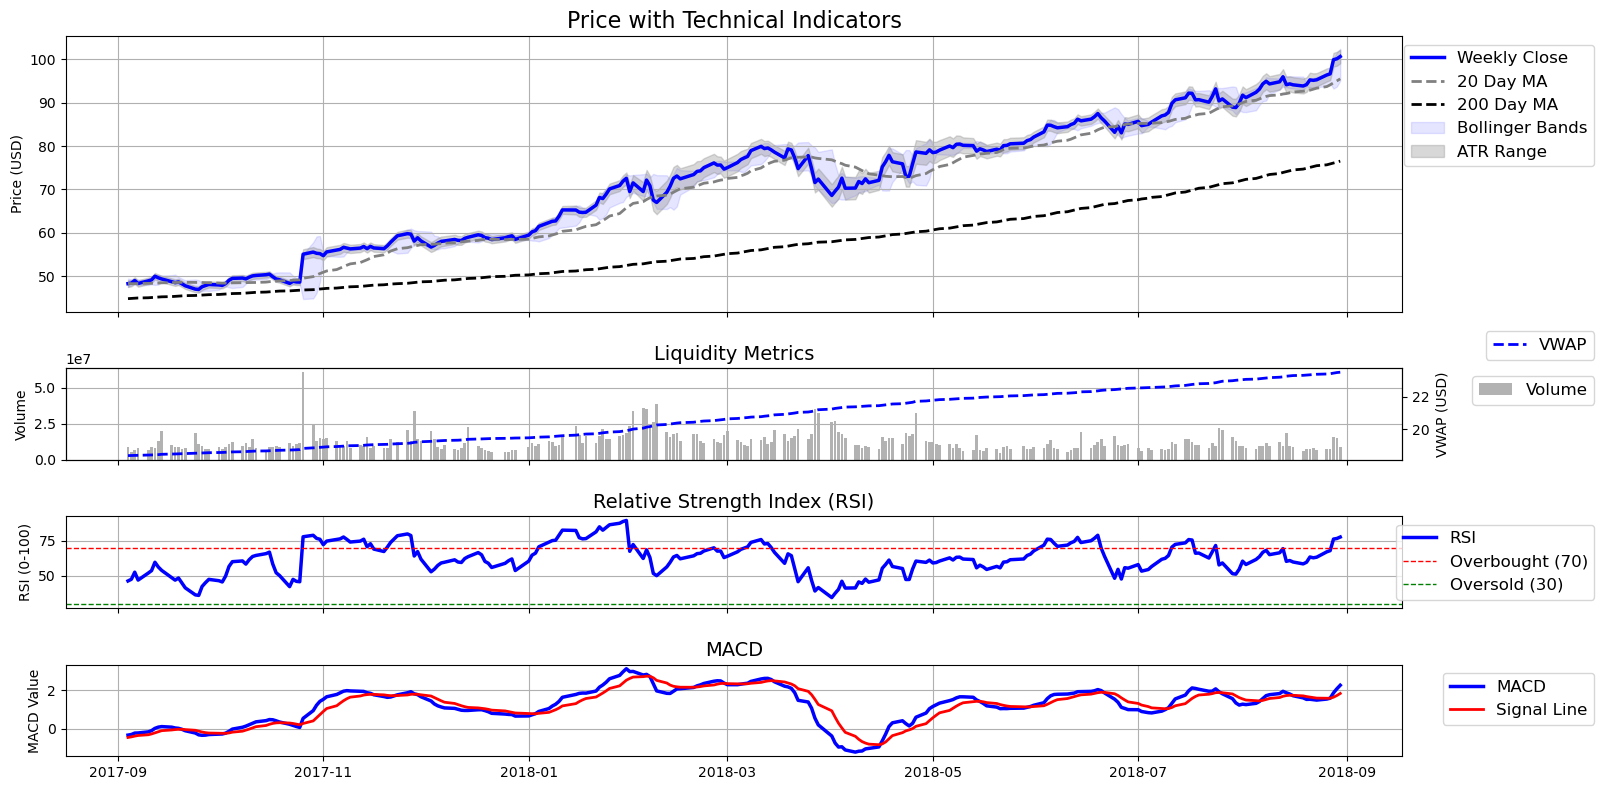
\includegraphics[width=1\linewidth]{judge_reviews//AMZN_M_gpt-4o-mini//2018-09-01/judge_Price_with_Technical_Indicators.png}
    \caption{Price and Technicals}
\end{figure}

\begin{figure}[H]
    \centering
    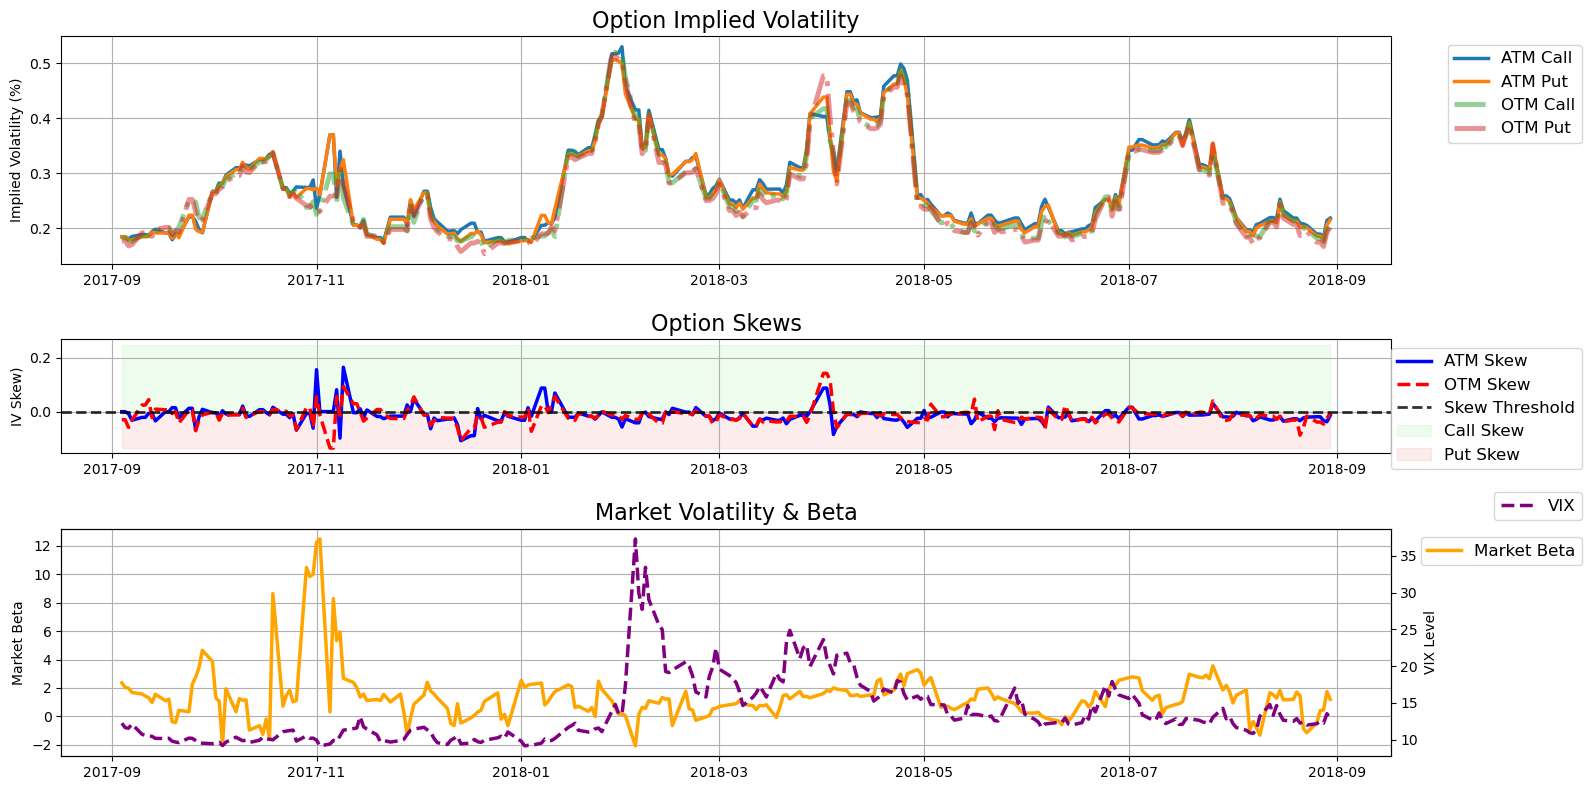
\includegraphics[width=1\linewidth]{judge_reviews/AMZN_M_gpt-4o-mini/2018-09-01/judge_Option_Implied_Volatility.png}
    \caption{Options}
\end{figure}

\begin{figure}[H]
    \centering
    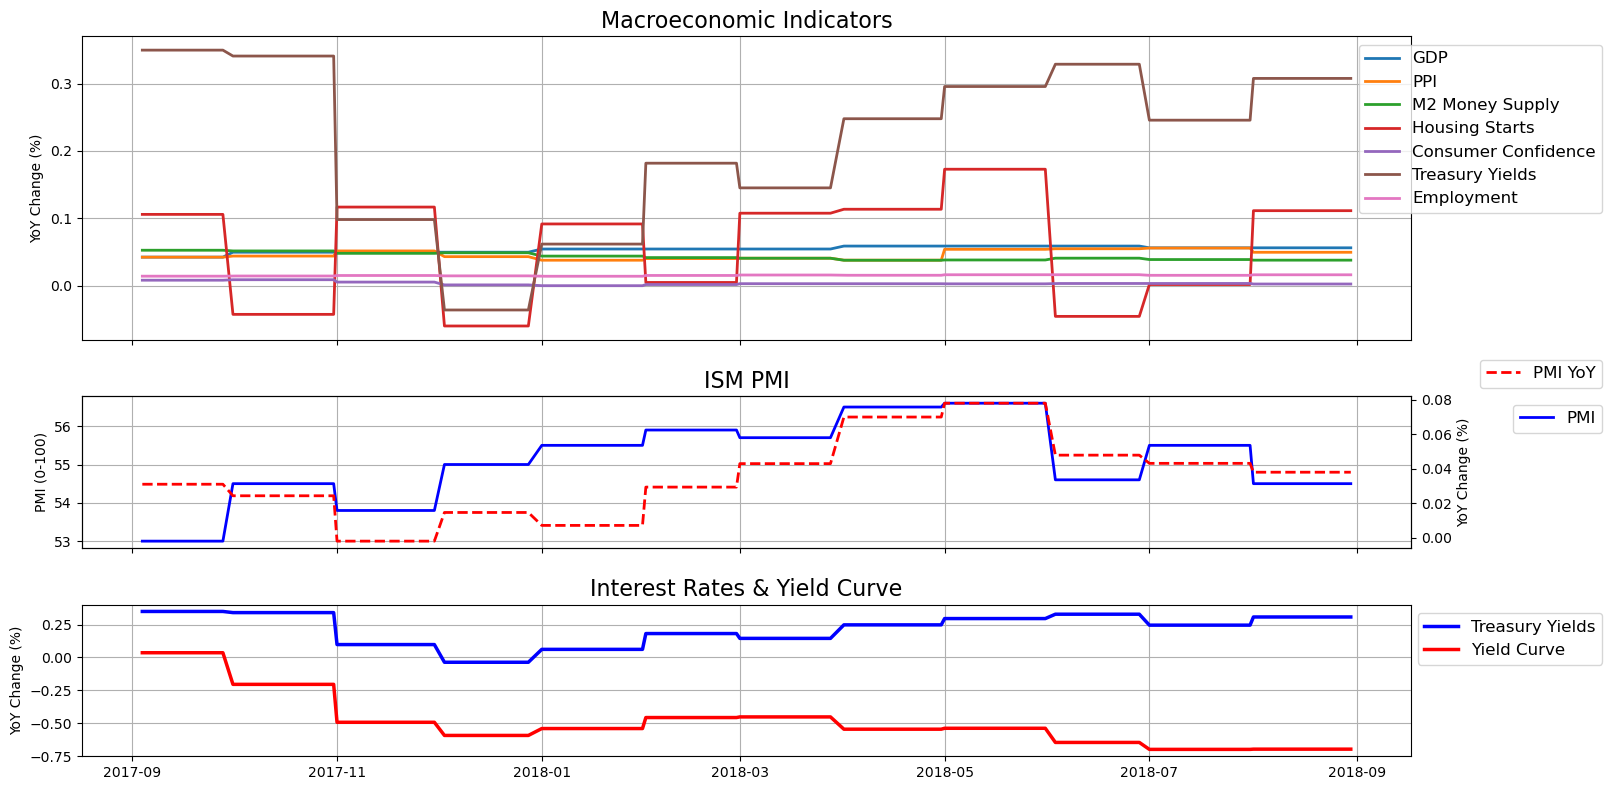
\includegraphics[width=1\linewidth]{judge_reviews/AMZN_M_gpt-4o-mini/2018-09-01/judge_Macroeconomic_Indicators.png}
    \caption{Macroeconomic}
\end{figure}

\begin{figure}[H]
    \centering
    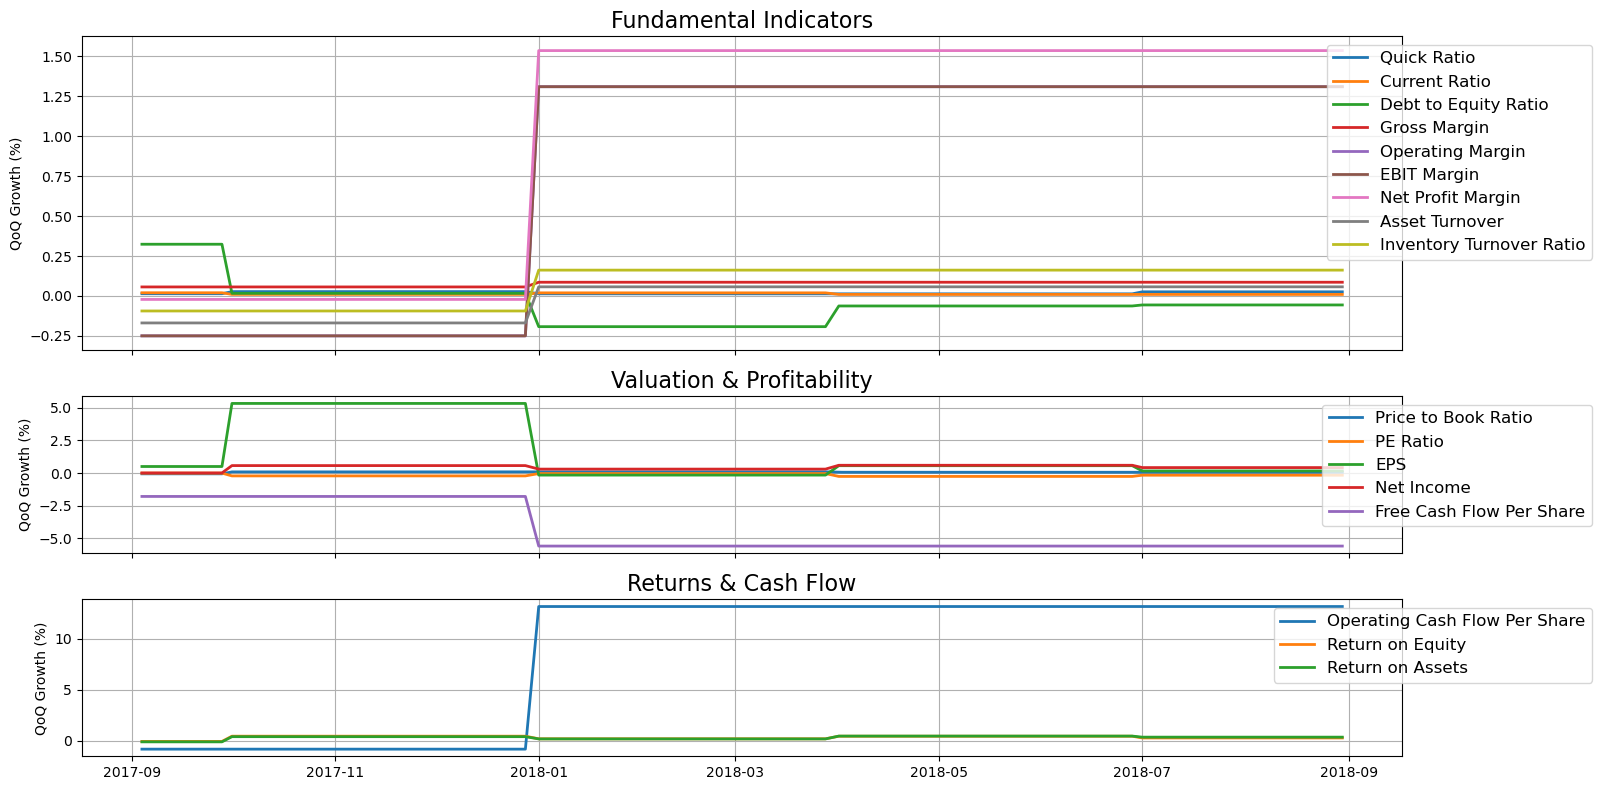
\includegraphics[width=1\linewidth]{judge_reviews/AMZN_M_gpt-4o-mini/2018-09-01/judge_Fundamental_Indicators.png}
    \caption{Fundamentals}
\end{figure}

\subsection*{Historic 1 Month News}

\textbf{Retail Sector Volatility and THE COMPANY’s Market Position}
Amid ongoing shifts in the retail landscape, THE COMPANY has faced increasing competitive pressure from digital retailers, leading to significant fluctuations in stock performance. Recent industry-wide movements have shown that investors are using THE COMPANY as a key indicator for traditional retail stability. Analysts suggest that continued adaptation to e-commerce trends will be crucial for THE COMPANY’s future growth.

\textbf{Strategic Expansion into Direct-to-Consumer Sales}
THE COMPANY has strengthened its focus on direct-to-consumer sales, enhancing its online platform and reducing reliance on third-party distribution. This shift has resulted in improved margins and greater control over customer engagement. Analysts believe that this strategy could protect THE COMPANY from broader market shifts while ensuring sustained revenue growth.

\textbf{Executive Leadership Changes and Market Reactions}
THE COMPANY announced key executive leadership changes, appointing a new senior figure to lead innovation and digital transformation efforts. The market reacted positively to the appointment, with investors expressing confidence in the company’s renewed focus on operational efficiency and strategic growth.

\textbf{Increased Competition in Key Market Segments}
Recent reports indicate that THE COMPANY is facing heightened competition in one of its core market segments, with rival firms aggressively expanding their offerings. Analysts predict that maintaining brand strength and customer loyalty will be critical to counteracting these competitive threats.

\textbf{Analyst Upgrades Amid Optimistic Growth Projections}
Several analysts have revised their outlook on THE COMPANY, citing improvements in product innovation, operational efficiency, and supply chain management. The stock price saw an upward movement following the revised projections, reflecting renewed investor confidence in the company’s long-term strategy.

\begin{tcolorbox}[colback=blue!10, colframe=blue!60, title=\textbf{TASKS}, sharp corners=southwest]
\begin{enumerate}
    \item Guess the action to take: \textit{LONG} or \textit{SHORT}.
    \item Write a 1-2 sentence \textit{explanation} on why you decided the action above.
\end{enumerate}
\end{tcolorbox}
\textbf{NEXT PAGE}: Model's Decision and Rationale.

\newpage

\subsection*{LLMs' Strategy} \label{strategy5}

The traded instrument was AMZN, with the trading period set between 2018-09-03 and 2019-10-01.

\textbf{LLMs' decision: \textit{LONG}}

\textbf{Rationale}: The analysis supports a LONG position based on several compelling indicators. Firstly, the stock is currently trading above its 20MA (90.00) and 50MA (86.47), signaling positive momentum with a recent close at 91.72, indicating strength in price action. Secondly, the RSI value of 60.43 suggests that while the stock is not overbought yet, it is trending positively which could indicate further upside potential.

Thirdly, despite some mixed analyst views regarding valuation and short-term volatility due to trade tensions and tariffs, there are also positive indicators such as analyst upgrades for THE COMPANY’s stock target suggesting expected growth, which impacts sentiment positively.

From a fundamental perspective, EPS YoY growth of approximately 8.67\% indicates solid profitability trends, even though free cash flow has seen negative movement (-5.60\%), showing resilience in earnings generation under pressure.

Lastly, macro data showing SPX closing slope $>$ 0 and VIX slope $<$ 0 indicate bullish market sentiment overall, further reinforcing our decision.

\textbf{Top weighted features influencing this decision}:
\begin{enumerate}
    \item Stock\_Data.Price.Close (91.72)
    \item Technical\_Analysis.RSI.Value (60.43)
    \item Fundamental\_Data.Growth\_Metrics.EPS\_YoY (8.67\%)
    \item Moving_Averages.50MA (86.47)
    \item Macro\_Data.Market_Sentiment (Bullish)
\end{enumerate}

\textbf{Key news impacting this strategy}:
\begin{enumerate}
    \item THE COMPANY reached a \$1 trillion market cap post-Prime Day, boosting sales - Market Impact Score: 5/5
    \item Analyst upgrades suggest continued growth expectations - Market Impact Score: 4/5
    \item Launch of a new machine learning shopping platform enhances competitiveness - Market Impact Score: 3/5
\end{enumerate}

\textbf{LLM Decision Insights}

\begin{longtable}{l c}
\toprule
\textbf{LLM Decision Insights} & \textbf{Value} \\
\midrule
Long Probability & 0.75 \\
Short Probability & 0.25 \\
Perplexity & 2.38182e+29 \\
\midrule
Total Tokens & 46337 \\
Total Cost (USD) & \$0.007181 \\
\bottomrule
\end{longtable}

\subsection*{Following Month Data}

\textbf{Performance Metrics}

\begin{longtable}{l c}
\toprule
\textbf{Metric} & \textbf{Value} \\
\midrule
Sharpe Ratio (Annualized SR) & -1.70178 \\
Portfolio Turnover (PTR) & 0 \\
Maximum Drawdown (MDD) & 0.0645225 \\
Mean Drawdown Duration (MDDur) & 10.5 \\
Cumulative Returns & -0.0334379 \\
\bottomrule
\end{longtable}

\begin{figure}[H]
    \centering
    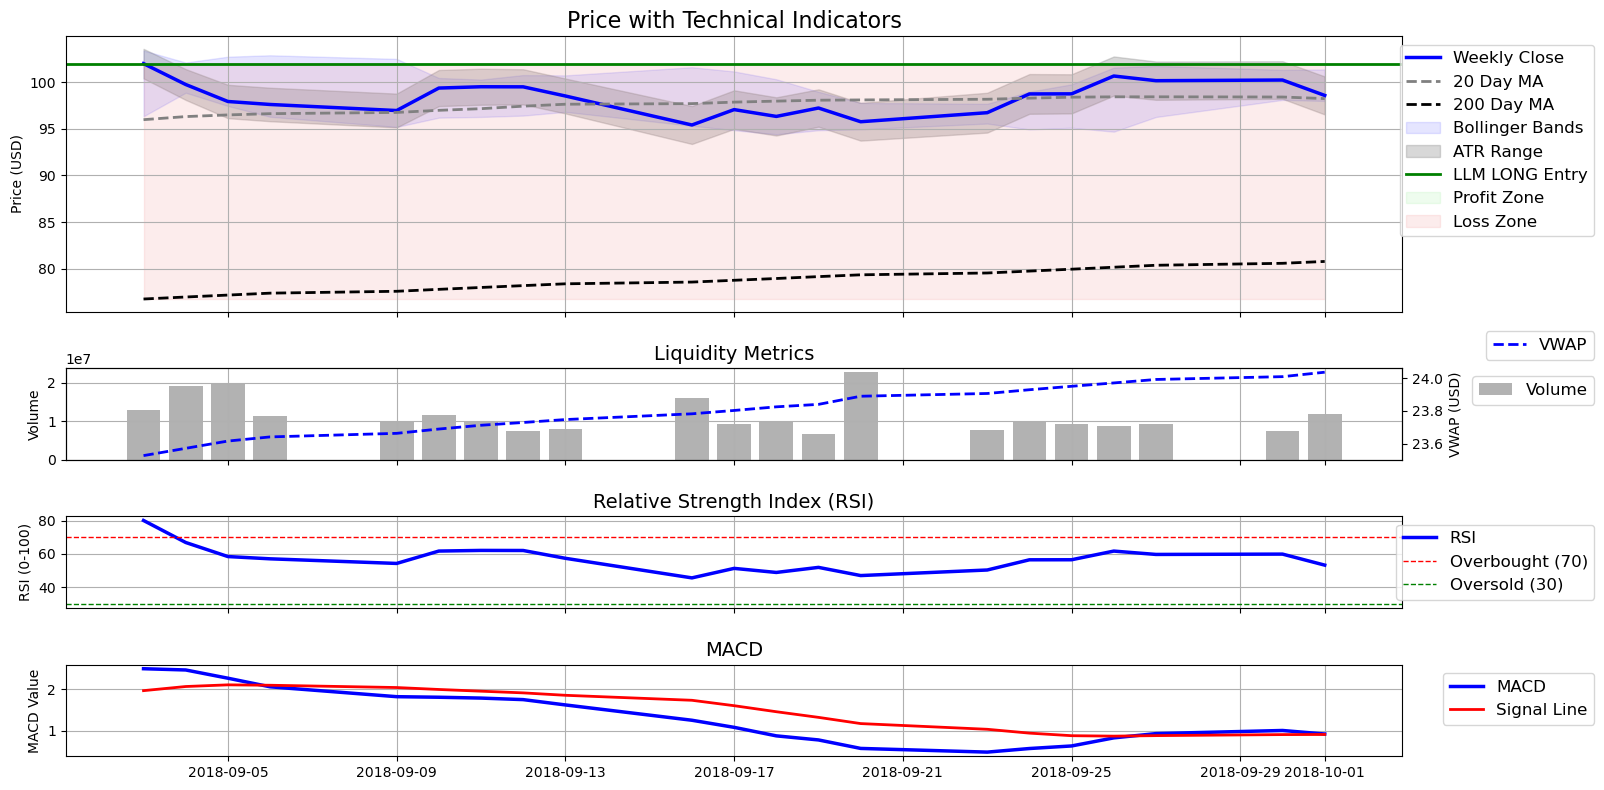
\includegraphics[width=1\linewidth]{judge_reviews//AMZN_M_gpt-4o-mini//2018-09-01/llm_Price_with_Technical_Indicators.png}
    \caption{Price after LLM's decision}
\end{figure}

\begin{figure}[H]
    \centering
    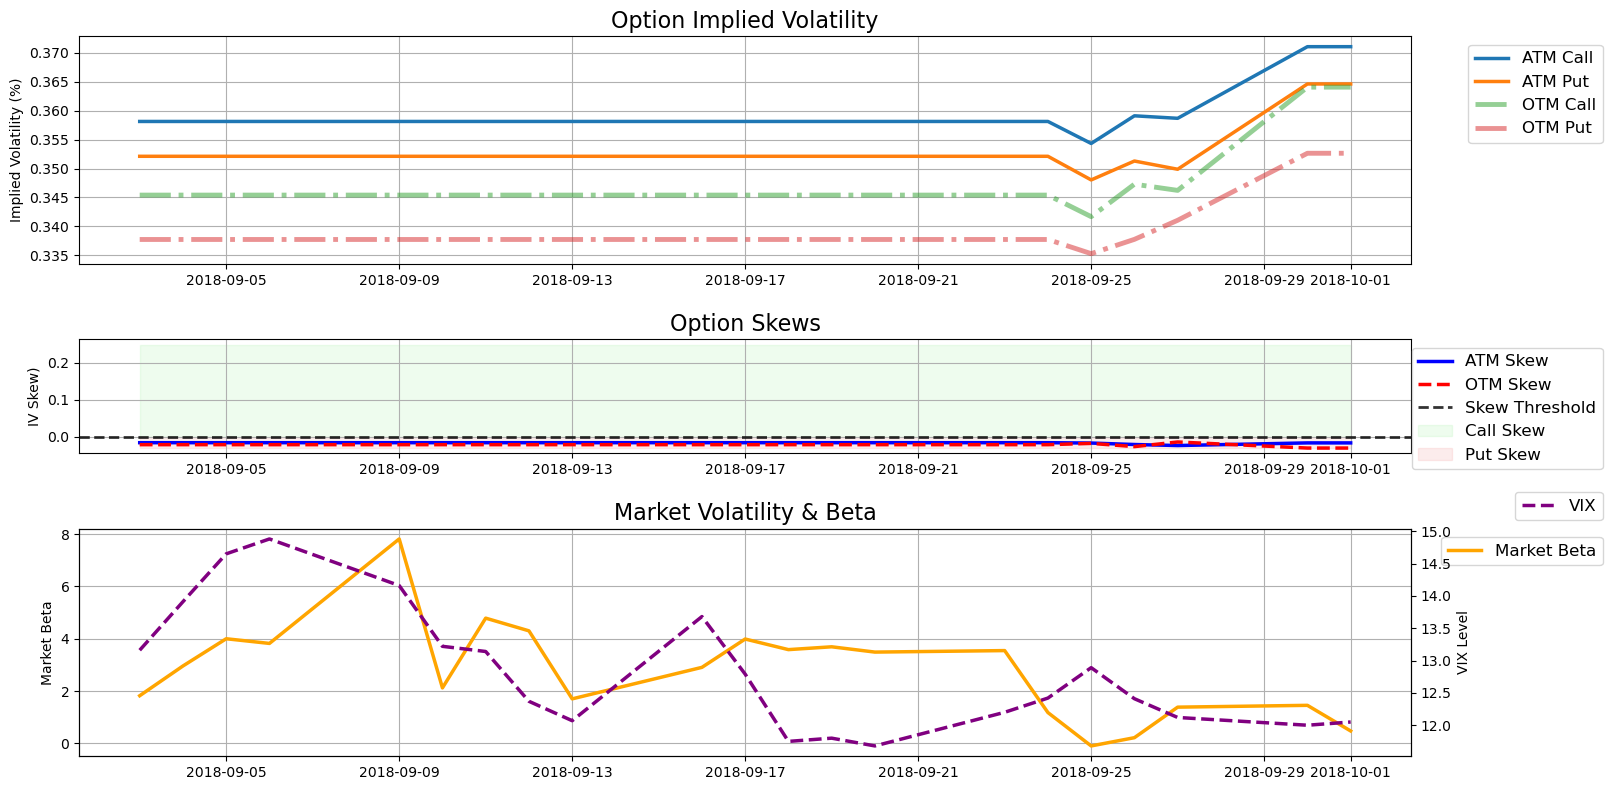
\includegraphics[width=1\linewidth]{judge_reviews/AMZN_M_gpt-4o-mini/2018-09-01/llm_Market_Volatility_&_Beta.png}
    \caption{Volatility after LLM's decision}
\end{figure}

\begin{tcolorbox}[colback=blue!10, colframe=blue!60, title=\textbf{TASKS}, sharp corners=southwest]
\begin{enumerate}
    \item Fill in the Expert Scoring \textit{rubric}.
    \item If applicable, provide \textit{examples} to correct the strategy.
\end{enumerate}
\end{tcolorbox}

\newpage


\section*{LLM Strategy 6}
\label{app:s6}

\subsection*{Historic 1 Year Data}

\begin{figure}[H]
    \centering
    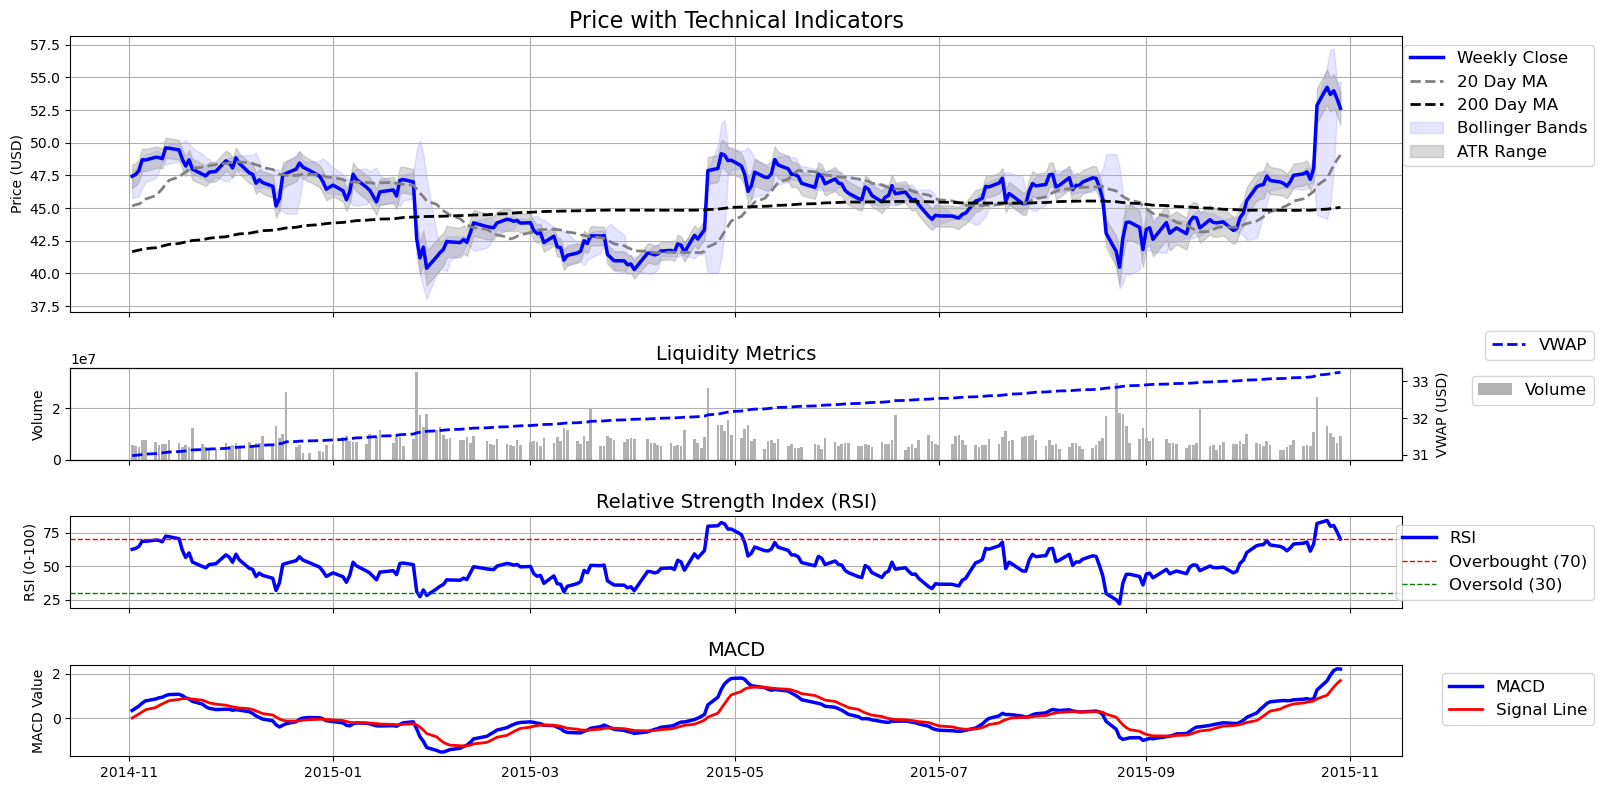
\includegraphics[width=1\linewidth]{judge_reviews/MSFT_M_gpt-4o-mini/2015-11-01/judge_Price_with_Technical_Indicators.png}
    \caption{Price and Technicals}
\end{figure}

\begin{figure}[H]
    \centering
    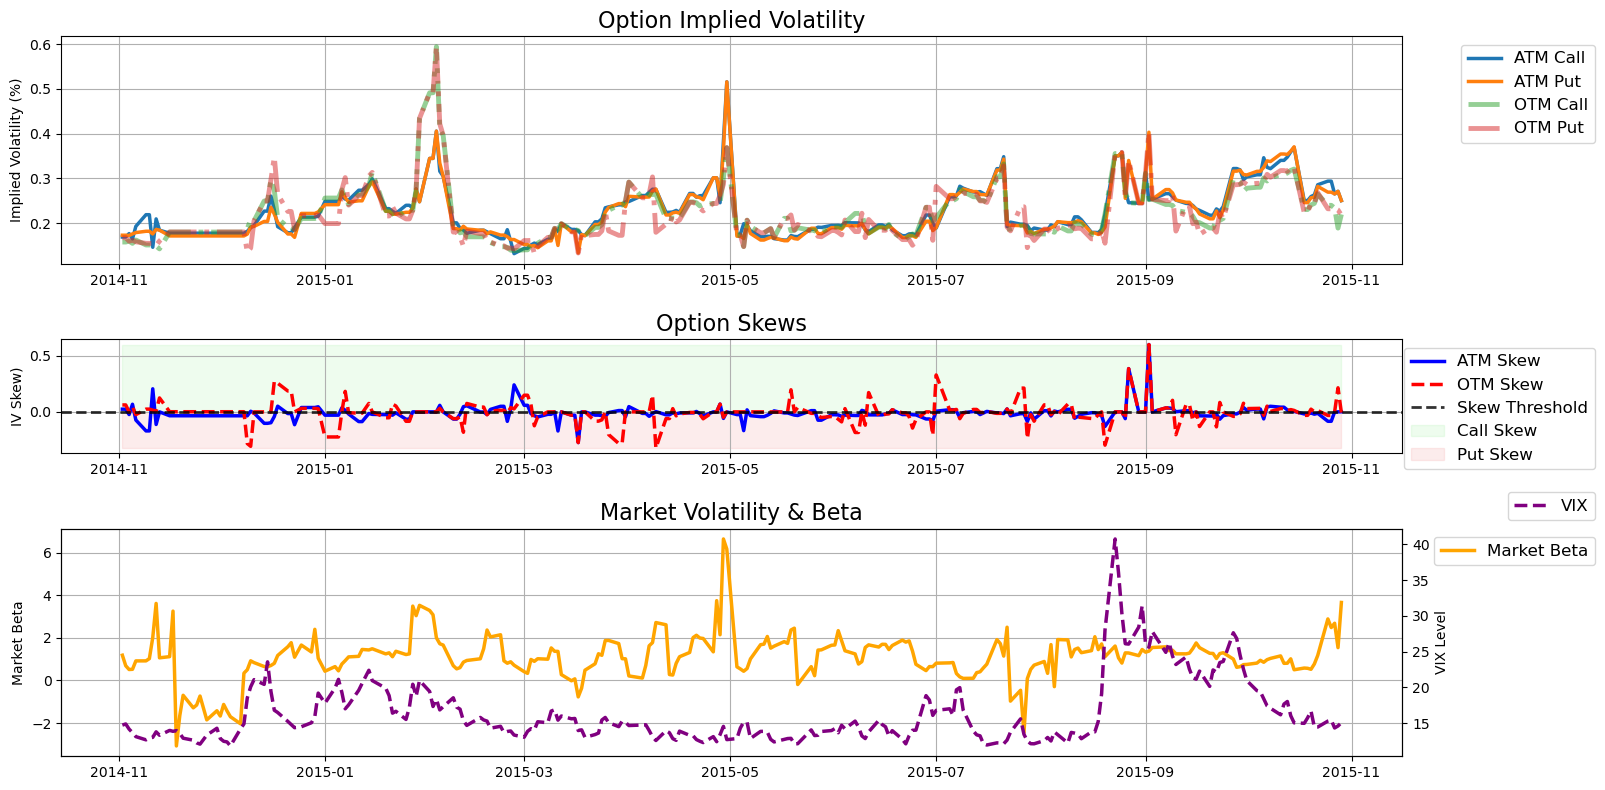
\includegraphics[width=1\linewidth]{judge_reviews/MSFT_M_gpt-4o-mini/2015-11-01/judge_Option_Implied_Volatility.png}
    \caption{Options}
\end{figure}

\begin{figure}[H]
    \centering
    \includegraphics[width=1\linewidth]{judge_reviews/MSFT_M_gpt-4o-mini/2015-11-01/judge_Macroeconomic_Indicators.png}
    \caption{Macroeconomic}
\end{figure}

\begin{figure}[H]
    \centering
    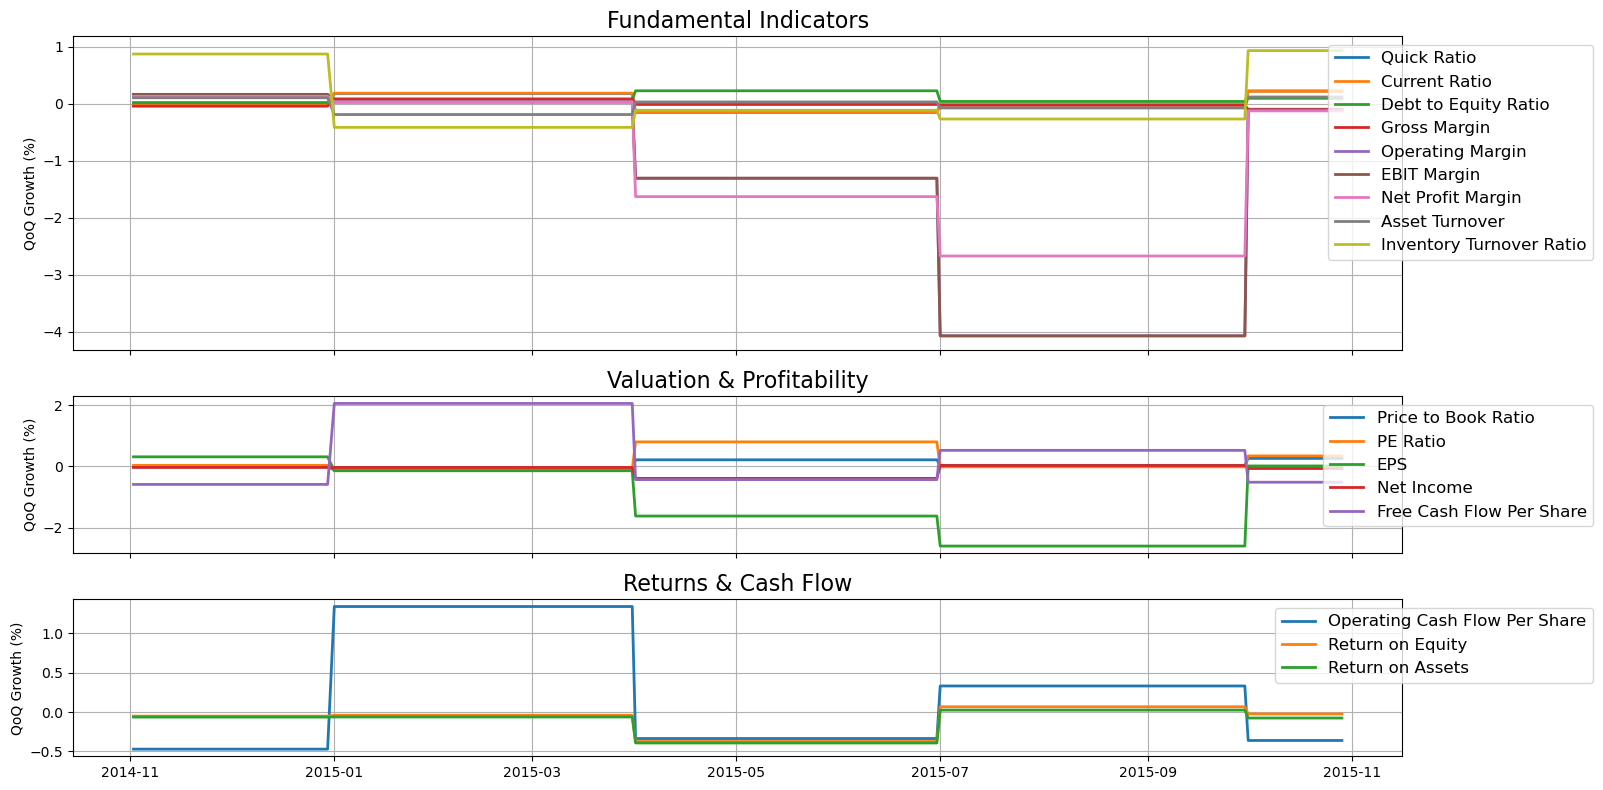
\includegraphics[width=1\linewidth]{judge_reviews/MSFT_M_gpt-4o-mini/2015-11-01/judge_Fundamental_Indicators.png}
    \caption{Fundamentals}
\end{figure}

\subsection*{Historic 1 Month News}

\textbf{Unusual Options Activity and Market Speculation}
Options traders exhibited significant bullish sentiment toward THE COMPANY, with heavy call buying activity ahead of an earnings report. Analysts speculated that this could signal confidence in strong financial performance and future growth prospects. This led to increased volatility and a short-term uptick in THE COMPANY's stock price.

\textbf{Leadership and Board Expansion}
THE COMPANY announced the nomination of two senior executives to its board of directors, reinforcing its strategic vision and corporate governance. The move was widely interpreted as an effort to strengthen leadership in key growth areas. Investor sentiment was cautiously optimistic, with market analysts viewing the expansion as a sign of long-term strategic planning.

\textbf{Earnings Beat and Strong Market Reaction}
THE COMPANY reported earnings that exceeded market expectations, with higher-than-expected revenue and improved profit margins. The announcement led to a sharp increase in its stock price in after-hours trading, as investors reacted positively to the financial results and management’s forward guidance.

\textbf{Technical Breakout and Analyst Projections}
Market analysts highlighted a bullish technical pattern in THE COMPANY's stock price, indicating a potential breakout. Comparisons were drawn to a major industry peer, suggesting that THE COMPANY could experience significant upside movement. The report fueled further investor optimism, leading to increased trading volume and a positive market response.

\textbf{Strategic Partnership in Emerging Technology}
THE COMPANY announced a collaboration with a major industry player to enhance its presence in emerging technology sectors. The partnership was positioned as a key strategic move to expand its ecosystem and strengthen its competitive position. Market participants reacted positively, seeing the deal as a catalyst for future revenue growth and innovation.


\textbf{TASKS}:

\begin{tcolorbox}[colback=blue!10, colframe=blue!60, title=\textbf{TASKS}, sharp corners=southwest]
\begin{enumerate}
    \item Guess the action to take: \textit{LONG} or \textit{SHORT}.
    \item Write a 1-2 sentence \textit{explanation} on why you decided the action above.
\end{enumerate}
\end{tcolorbox}

\newpage

\subsection*{LLMs' Strategy} \label{strategy6}

The traded instrument was MSFT, with the trading period set between 2015-11-02 and 2015-11-30.

\textbf{LLMs' decision: \textit{LONG}}

\textbf{Rationale}: The decision to take a LONG position is supported by multiple key factors. Firstly, THE COMPANY's stock is trading at \$45.57, above both the 20-day moving average (43.81) and the 50-day moving average (44.74), indicating strong bullish momentum. While historical volatility is relatively high (40\%), the implied volatility (27\%) suggests that market sentiment remains stable, providing an opportunity for controlled risk.

Secondly, technical indicators such as RSI at 60.18 suggest further upside potential before overbought conditions set in. Fundamentally, despite a decline in EPS YoY (-12.68\%), free cash flow growth of 28.99\% highlights strong liquidity and operational efficiency, reinforcing the bullish case.

Macroeconomic conditions also favor a long position, with GDP QoQ at 0.18\% and declining market volatility (VIX down 7\%), indicating a risk-on sentiment. The broader market (SPX) is also in an upward trend (+1\%), adding further confidence in equities.

\textbf{Top weighted features influencing this decision}:
\begin{enumerate}
    \item Stock\_Data.Price.Close (45.57)
    \item Technical\_Analysis.MACD.Value (0.312)
    \item Fundamental\_Data.Growth\_Metrics.Free\_Cash\_Flow\_YoY (28.99\%)
    \item Technical\_Analysis.RSI (60.18)
    \item Market\_Data.SPX.Slope (+1\%)
\end{enumerate}

\textbf{Key news impacting this strategy}:
\begin{enumerate}
    \item Earnings expectations from major companies expected to positively influence stock prices - Market Impact Score: 5/5
    \item Mixed performance in overall earnings season could favor THE COMPANY if it meets estimates - Market Impact Score: 4/5
    \item Analysts predicting challenges yet potentially manageable impacts on flagship product demand - Market Impact Score: 3/5
\end{enumerate}


\begin{longtable}{l c}
\toprule
\textbf{LLM Decision Insights} & \textbf{Value} \\
\midrule
Long Probability & 0.82 \\
Short Probability & 0.18 \\
\midrule
Total Tokens & 17744 \\
Total Cost (USD) & \$0.002885 \\
\bottomrule
\end{longtable}

\subsection*{Following Month Data}

\textbf{Performance Metrics}

\begin{longtable}{l c}
\toprule
\textbf{Metric} & \textbf{Value} \\
\midrule
Sharpe Ratio (Annualized SR) & 1.47043 \\
Portfolio Turnover (PTR) & 0 \\
Maximum Drawdown (MDD) & 0.0378733 \\
Mean Drawdown Duration (MDDur) & 7.17647 \\
Cumulative Returns & 0.0195753 \\
\bottomrule
\end{longtable}


\begin{figure}[H]
    \centering
    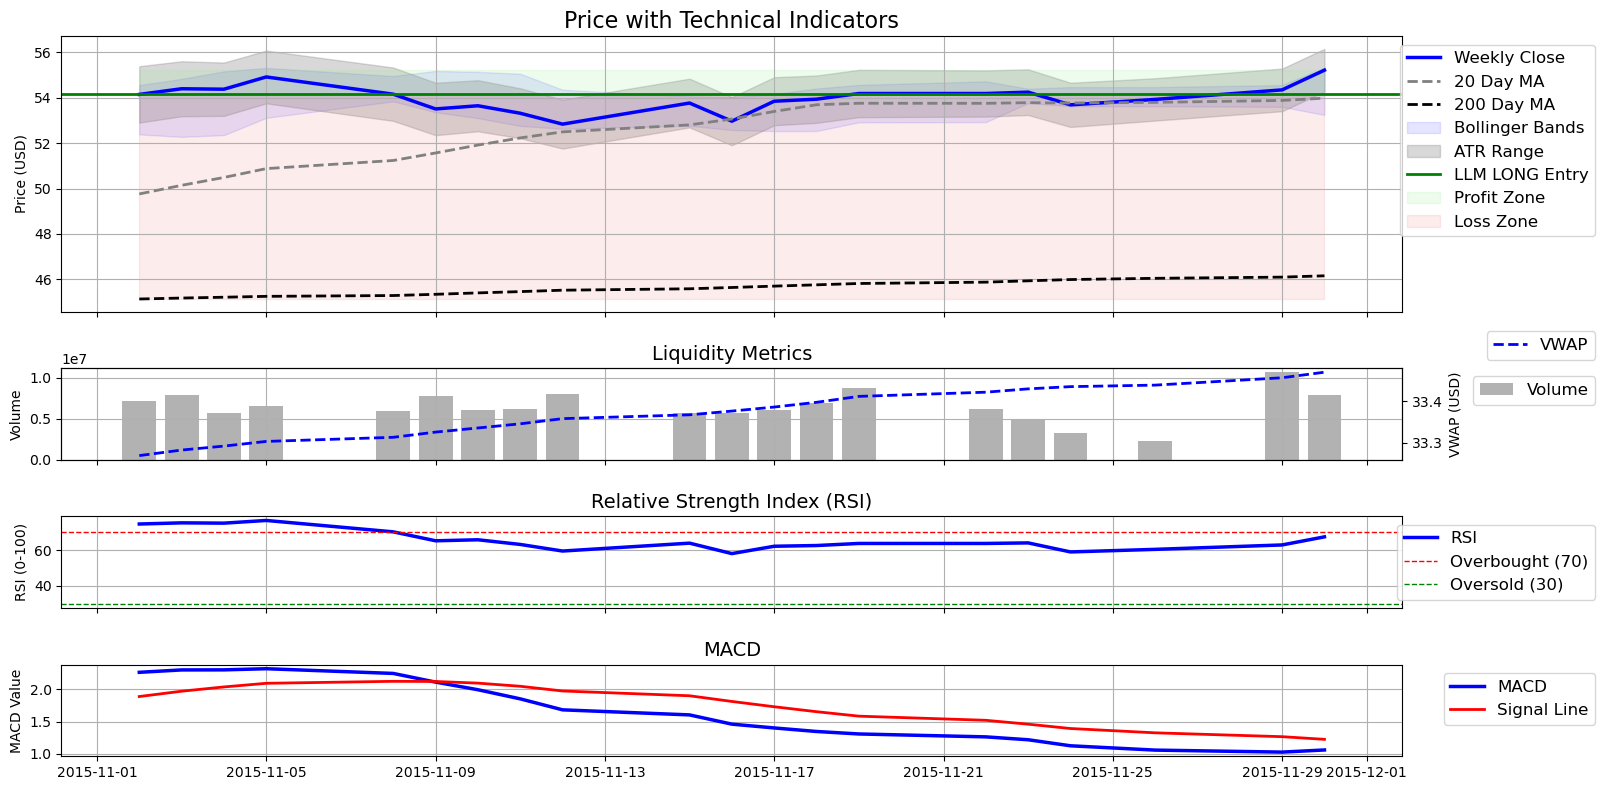
\includegraphics[width=1\linewidth]{judge_reviews/MSFT_M_gpt-4o-mini//2015-11-01/llm_Price_with_Technical_Indicators.png}
    \caption{Price after LLM's decision}
\end{figure}

\begin{figure}[H]
    \centering
    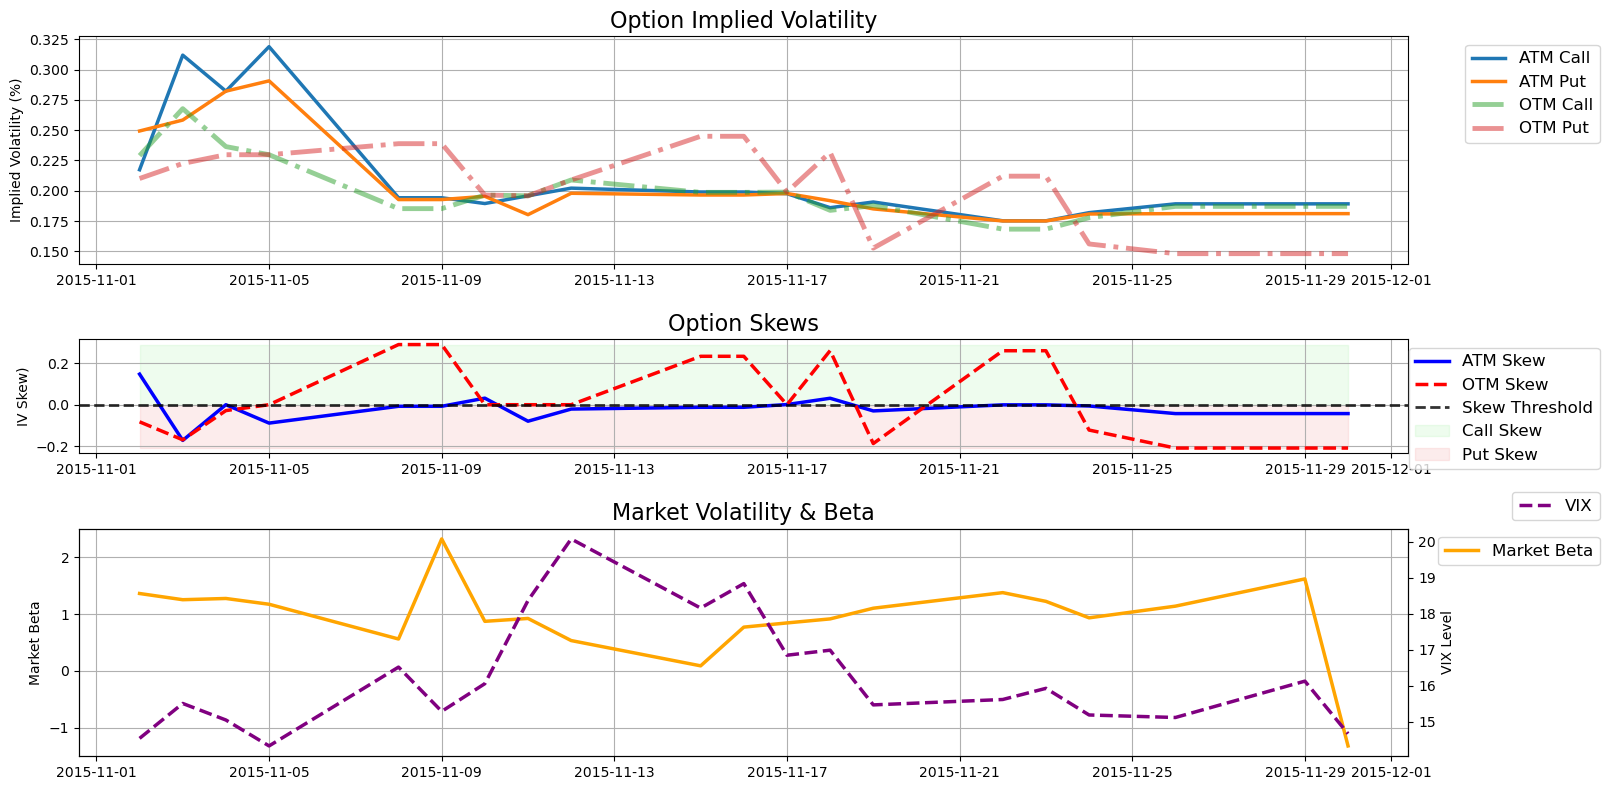
\includegraphics[width=1\linewidth]{judge_reviews/MSFT_M_gpt-4o-mini/2015-11-01/llm_Market_Volatility_&_Beta.png}
    \caption{Volatility after LLM's decision}
\end{figure}

\begin{tcolorbox}[colback=blue!10, colframe=blue!60, title=\textbf{TASKS}, sharp corners=southwest]
\begin{enumerate}
    \item Fill in the Expert Scoring \textit{rubric}.
    \item If applicable, provide \textit{examples} to correct the strategy.
\end{enumerate}
\end{tcolorbox}
\newpage


\section*{LLM Strategy 7}
\label{app:s7}
\subsection*{Historic 1 Year Data}

\begin{figure}[H]
    \centering
    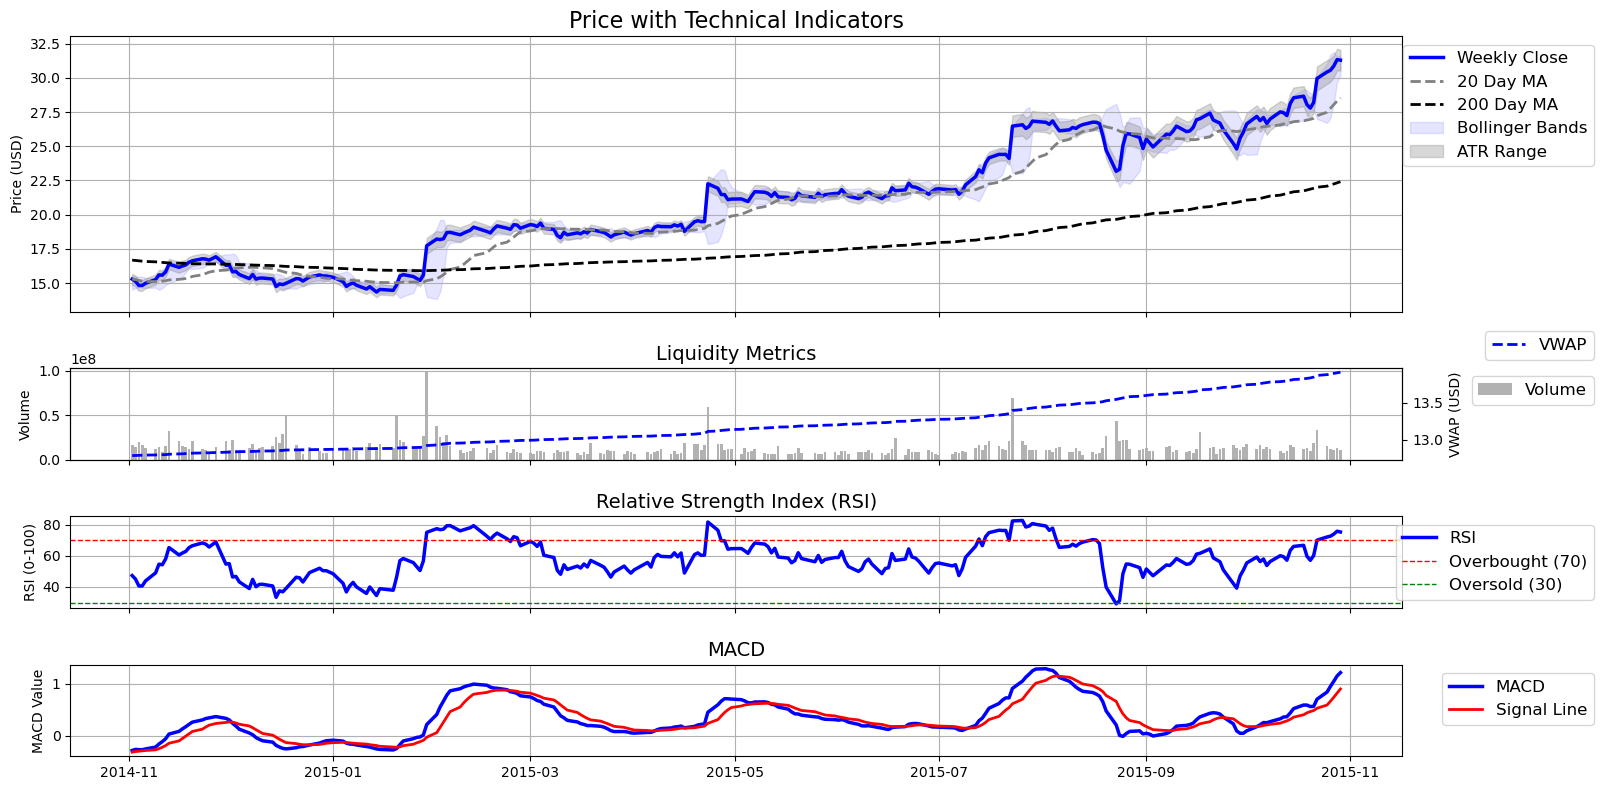
\includegraphics[width=1\linewidth]{judge_reviews/AMZN_M_gpt-4o-mini/2015-11-01/judge_Price_with_Technical_Indicators.png}
    \caption{Price and Technicals}
\end{figure}

\begin{figure}[H]
    \centering
    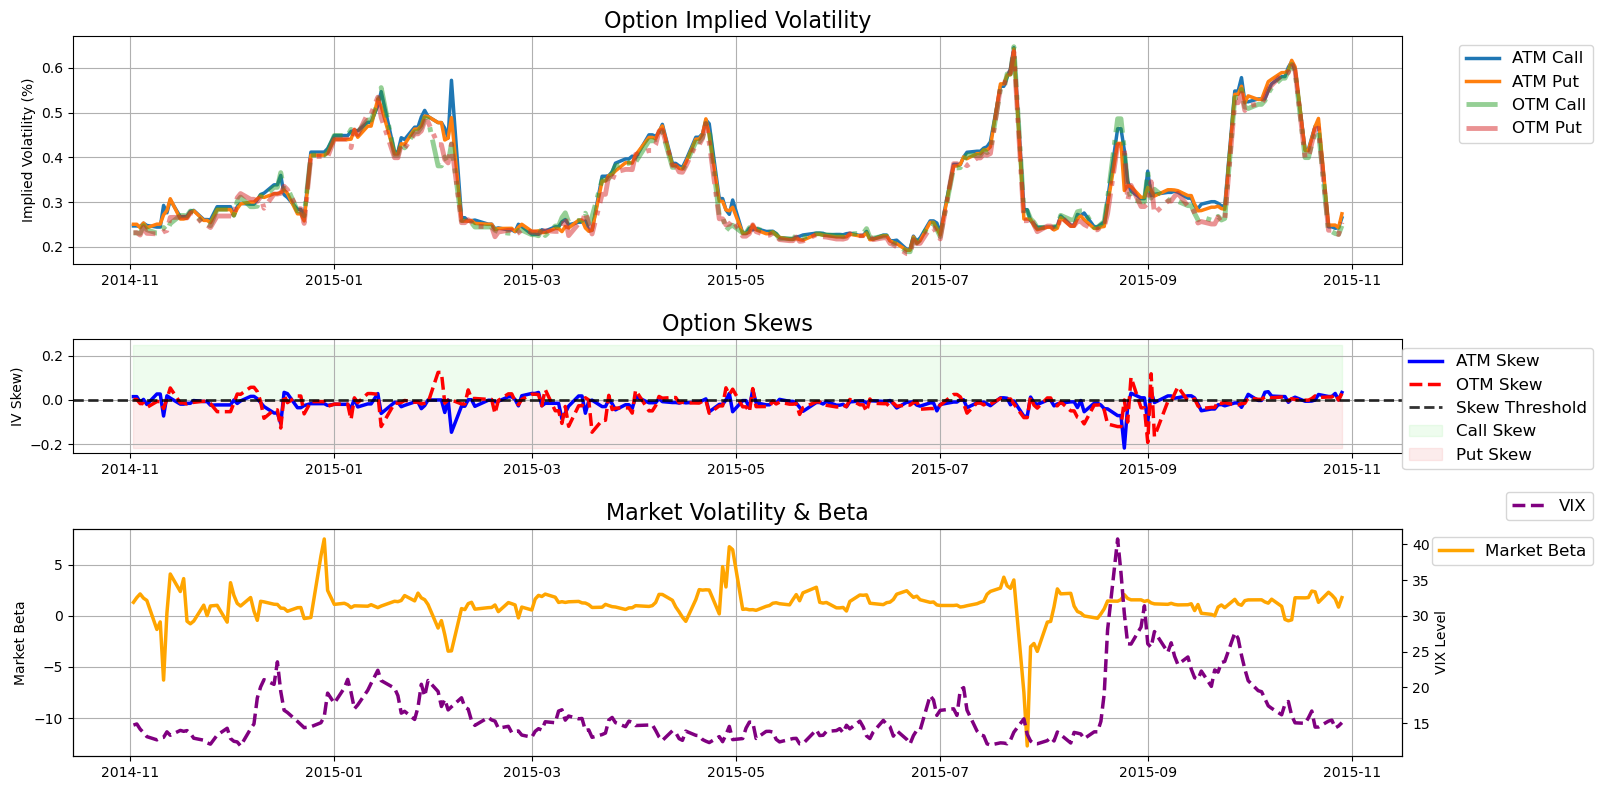
\includegraphics[width=1\linewidth]{judge_reviews/AMZN_M_gpt-4o-mini/2015-11-01/judge_Option_Implied_Volatility.png}
    \caption{Options}
\end{figure}

\begin{figure}[H]
    \centering
    \includegraphics[width=1\linewidth]{judge_reviews/AMZN_M_gpt-4o-mini/2015-11-01/judge_Macroeconomic_Indicators.png}
    \caption{Macroeconomic}
\end{figure}

\begin{figure}[H]
    \centering
    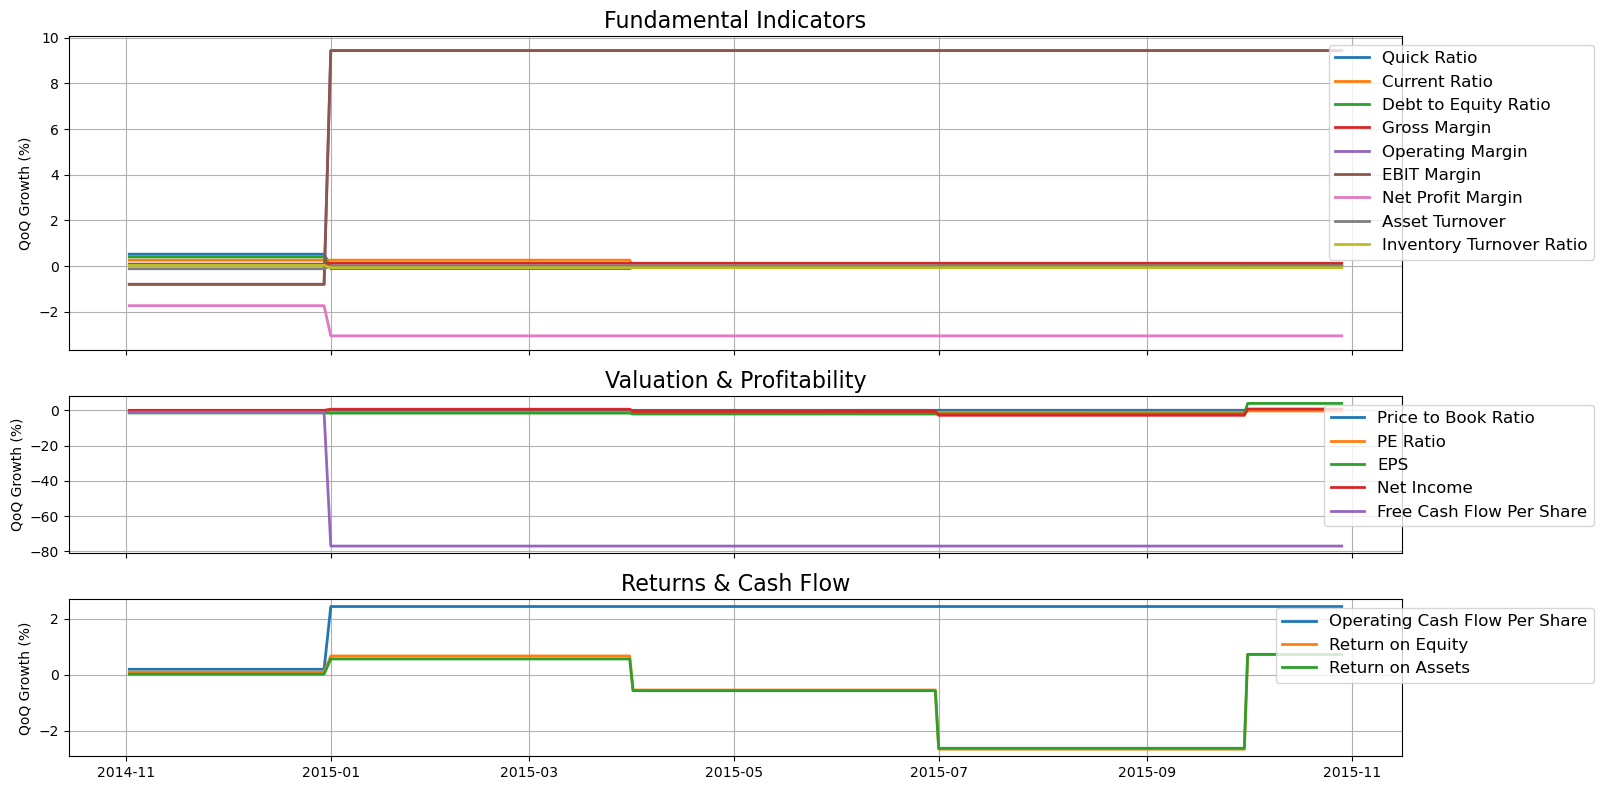
\includegraphics[width=1\linewidth]{judge_reviews/AMZN_M_gpt-4o-mini/2015-11-01/judge_Fundamental_Indicators.png}
    \caption{Fundamentals}
\end{figure}

\subsection*{Historic 3 Month News}

\textbf{Strong Financial Performance \& Earnings Beat}
THE COMPANY reported a significant earnings beat, posting revenue and profit figures well above analysts’ expectations. The surprise profitability fueled a sharp increase in THE COMPANY’s stock price, surging over 10\% in after-hours trading. Investors reacted positively to the strong growth across multiple segments, particularly in cloud services and digital media.

\textbf{Work Culture Controversy \& Public Backlash}
A major publication released an investigative report criticizing THE COMPANY’s workplace culture, citing allegations of excessive pressure, harsh management practices, and unfair treatment of employees. THE COMPANY’s top executives, including THE VP, issued a strong rebuttal, claiming the report was misleading and lacked journalistic standards. While the news initially weighed on investor sentiment, the company’s stock remained resilient amid continued business growth.

\textbf{Expansion in Logistics \& Delivery Services}
THE COMPANY announced the expansion of its same-day delivery service to multiple metropolitan areas, increasing its footprint in the logistics space. The move was seen as a direct challenge to traditional courier services and positioned THE COMPANY as a dominant force in e-commerce fulfillment. Analysts viewed the expansion favorably, citing enhanced customer experience and potential cost efficiencies.

\textbf{Major Hiring Initiative for Seasonal Workforce}
Ahead of the holiday season, THE COMPANY revealed plans to hire over 100,000 temporary workers to meet rising demand. The announcement signaled confidence in consumer spending and THE COMPANY’s ability to handle peak shopping periods. Market reaction was positive, with analysts expecting a strong quarter driven by increased retail sales.

\textbf{Regulatory Scrutiny Over Tax Practices}
THE COMPANY faced renewed scrutiny from regulatory bodies regarding its tax structure and alleged use of offshore subsidiaries to minimize tax obligations. While no immediate penalties were imposed, the heightened regulatory attention created some uncertainty for investors. However, the stock showed limited reaction as the broader market remained focused on the company's robust growth prospects.


\textbf{TASKS}:

\begin{tcolorbox}[colback=blue!10, colframe=blue!60, title=\textbf{TASKS}, sharp corners=southwest]
\begin{enumerate}
    \item Guess the action to take: \textit{LONG} or \textit{SHORT}.
    \item Write a 1-2 sentence \textit{explanation} on why you decided the action above.
\end{enumerate}
\end{tcolorbox}

\newpage

\subsection*{LLMs' Strategy} \label{strategy7}

The traded instrument was AMZN, with the trading period set between 2015-11-02 and 2015-11-30.

\textbf{LLMs' decision: \textit{LONG}}

\textbf{Rationale}: The analysis indicates a bullish sentiment for the stock based on several key factors.

1) \textbf{Technical Analysis}: The current price of 26.63 is above both the 20MA (26.20) and 50MA (26.07), indicating strong upward momentum. The RSI value at 55 suggests that the stock is neither overbought nor oversold, supporting potential further upside.

2) \textbf{Stock Performance}: Recent weekly returns show significant volatility with a cumulative return of approximately 1\% in recent weeks, suggesting positive market interest and possible trend sustainability.

3) \textbf{News Factors}: Analysts have raised their price target for the company due to underappreciated growth potential in its cloud services (Market Impact Score: 5). Additionally, early Black Friday deals announced by executives could significantly enhance sales (Score: 4). Lastly, the launch of brick-and-mortar stores leveraging online data can improve customer engagement (Score: 3). These news factors collectively support a bullish stance as they highlight strong growth narratives around profitability and revenue generation prospects amidst favorable technical indicators.

\textbf{Top weighted features influencing this decision}:
\begin{enumerate}
    \item Stock\_Data.Price.Close (26.63)
    \item Technical\_Analysis.RSI.Value (55)
    \item Technical\_Analysis.20MA (26.20)
    \item Technical\_Analysis.50MA (26.07)
    \item Fundamental\_Data.Growth\_Metrics.Revenue\_YoY (+21\%)
\end{enumerate}

\textbf{Key news impacting this strategy}:
\begin{enumerate}
    \item Official launch of first brick-and-mortar store leveraging online data for inventory - Market Impact Score: 3
    \item Analysts predict significant disruption in IT market due to cloud services growth - Market Impact Score: 5
    \item Announcement of extensive Black Friday deals with early access for premium members - Market Impact Score: 4
    \item Price target increase by major investment bank citing strong cloud division outlook - Market Impact Score: 5
    \item Major retailer transitions online store to THE COMPANY, reinforcing retail dominance - Market Impact Score: 3
\end{enumerate}

\textbf{LLM Decision Insights}

\begin{longtable}{l c}
\toprule
\textbf{LLM Decision Insights} & \textbf{Value} \\
\midrule
Long Probability & 0.75 \\
Short Probability & 0.25 \\
Perplexity & 1.92457 \\
\midrule
Total Tokens & 68462 \\
Total Cost (USD) & \$0.010503 \\
\bottomrule
\end{longtable}

\subsection*{Following Month Data}

\textbf{Performance Metrics}

\begin{longtable}{l c}
\toprule
\textbf{Metric} & \textbf{Value} \\
\midrule
Sharpe Ratio (Annualized SR) & 3.76259 \\
Portfolio Turnover (PTR) & 0 \\
Maximum Drawdown (MDD) & 0.0457516 \\
Mean Drawdown Duration (MDDur) & 3.57143 \\
Cumulative Returns & 0.0809082 \\
\bottomrule
\end{longtable}


\begin{figure}[H]
    \centering
    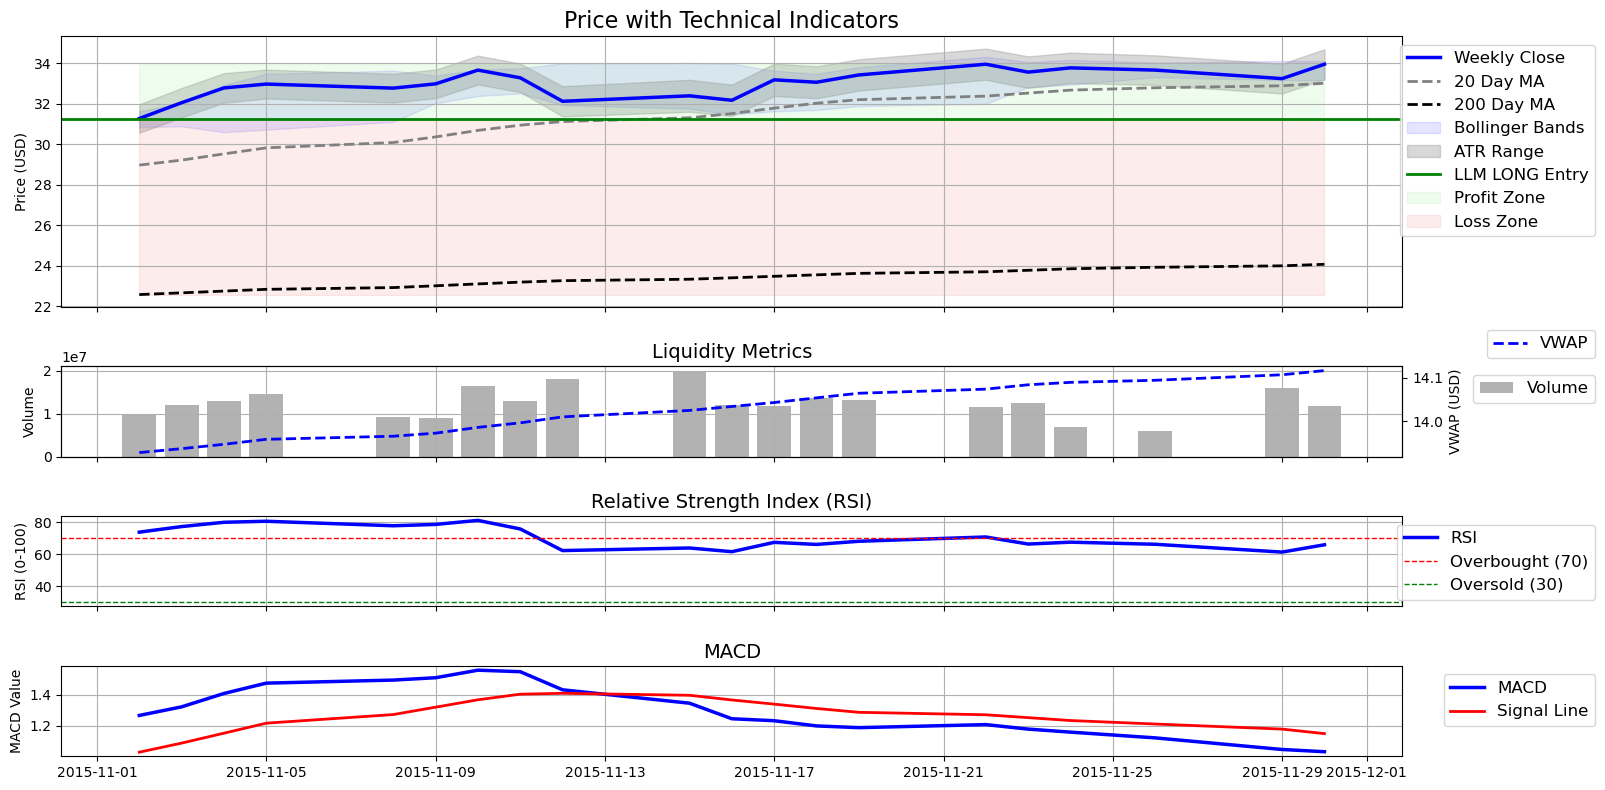
\includegraphics[width=1\linewidth]{judge_reviews/AMZN_M_gpt-4o-mini//2015-11-01/llm_Price_with_Technical_Indicators.png}
    \caption{Price after LLM's decision}
\end{figure}

\begin{figure}[H]
    \centering
    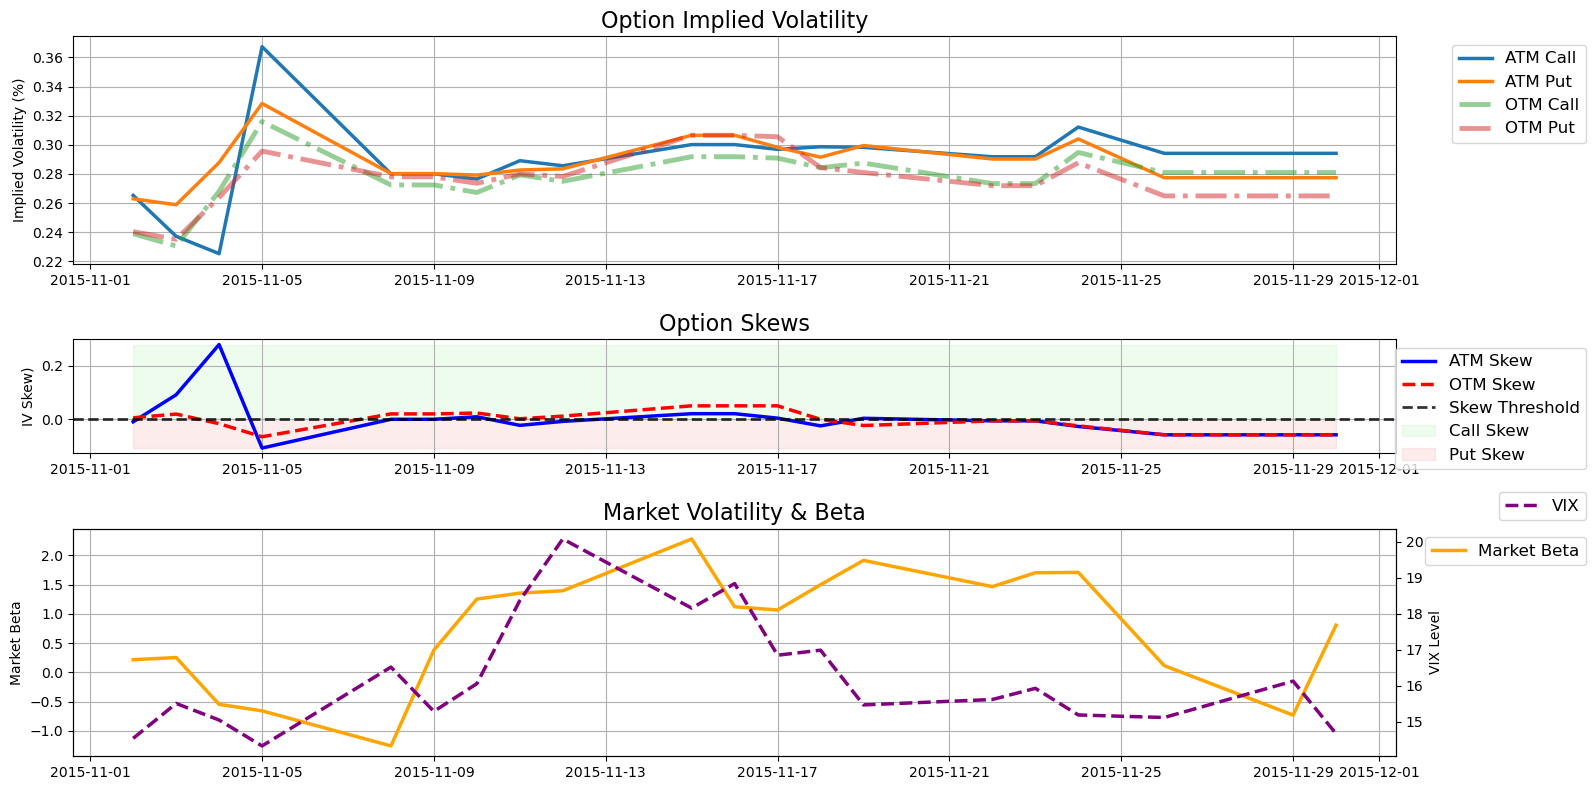
\includegraphics[width=1\linewidth]{judge_reviews/AMZN_M_gpt-4o-mini/2015-11-01/llm_Market_Volatility_&_Beta.png}
    \caption{Volatility after LLM's decision}
\end{figure}

\begin{tcolorbox}[colback=blue!10, colframe=blue!60, title=\textbf{TASKS}, sharp corners=southwest]
\begin{enumerate}
    \item Fill in the Expert Scoring \textit{rubric}.
    \item If applicable, provide \textit{examples} to correct the strategy.
\end{enumerate}
\end{tcolorbox}
\newpage



\section*{LLM Strategy 8}
\label{app:s8}

\subsection*{Historic 1 Year Data}

\begin{figure}[H]
    \centering
    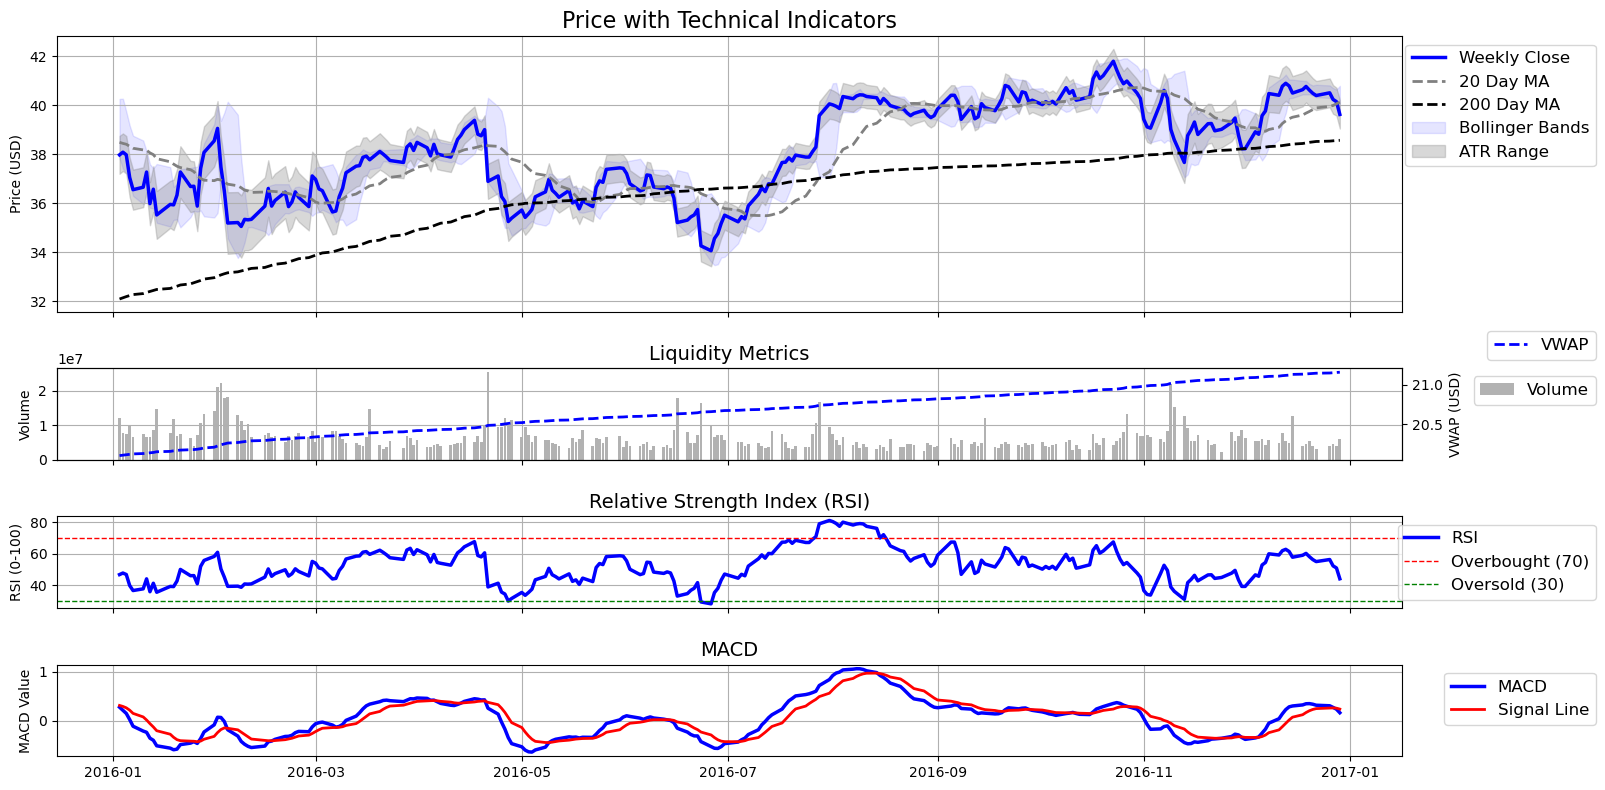
\includegraphics[width=1\linewidth]{judge_reviews/GOOGL_M_gpt-4o-mini//2017-01-01/judge_Price_with_Technical_Indicators.png}
    \caption{Price and Technicals}
\end{figure}

\begin{figure}[H]
    \centering
    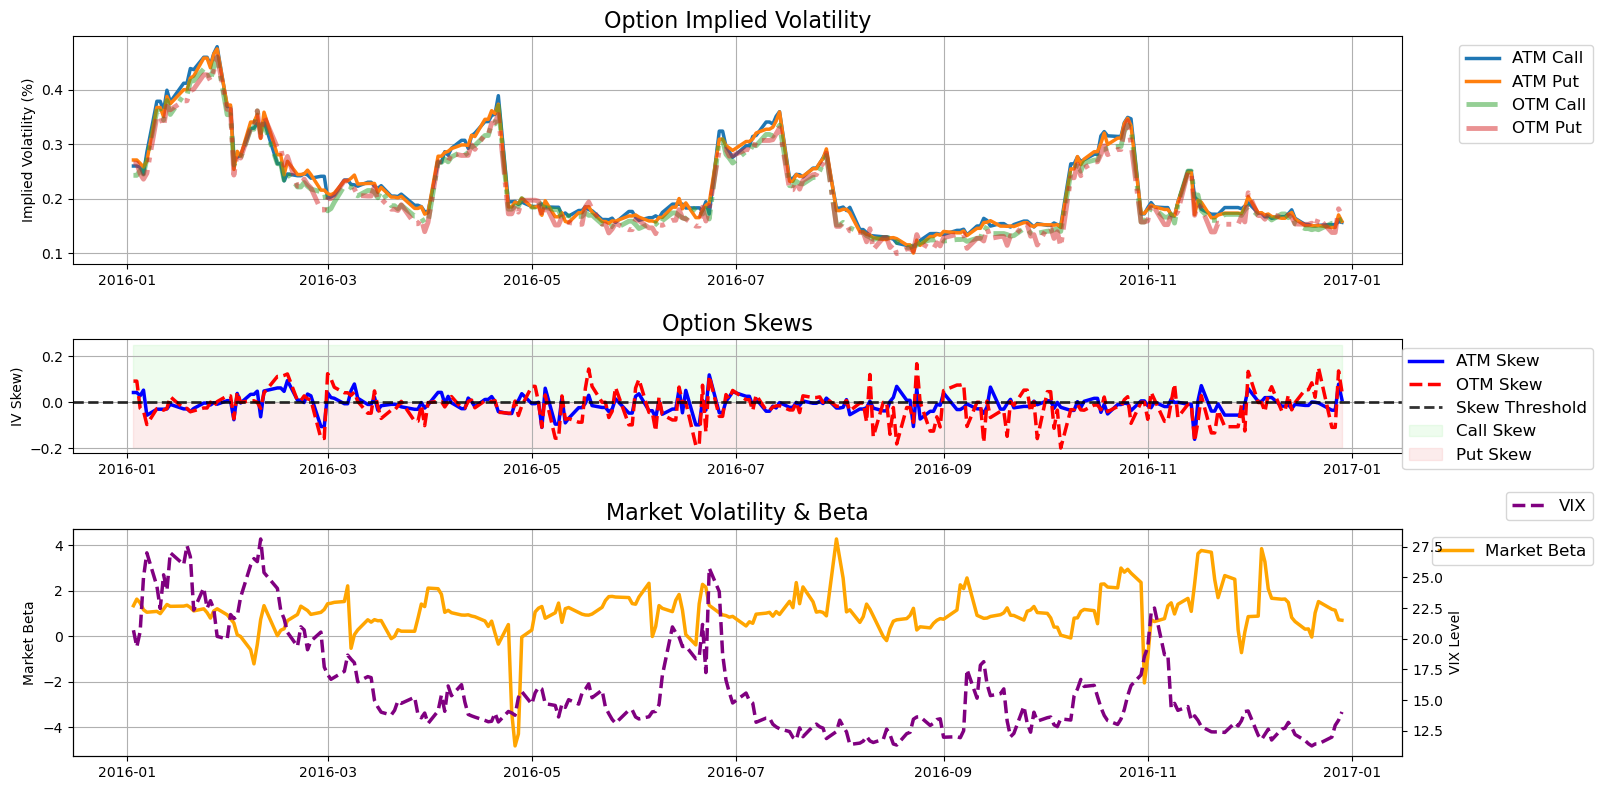
\includegraphics[width=1\linewidth]{judge_reviews/GOOGL_M_gpt-4o-mini/2017-01-01/judge_Option_Implied_Volatility.png}
    \caption{Options}
\end{figure}

\begin{figure}[H]
    \centering
    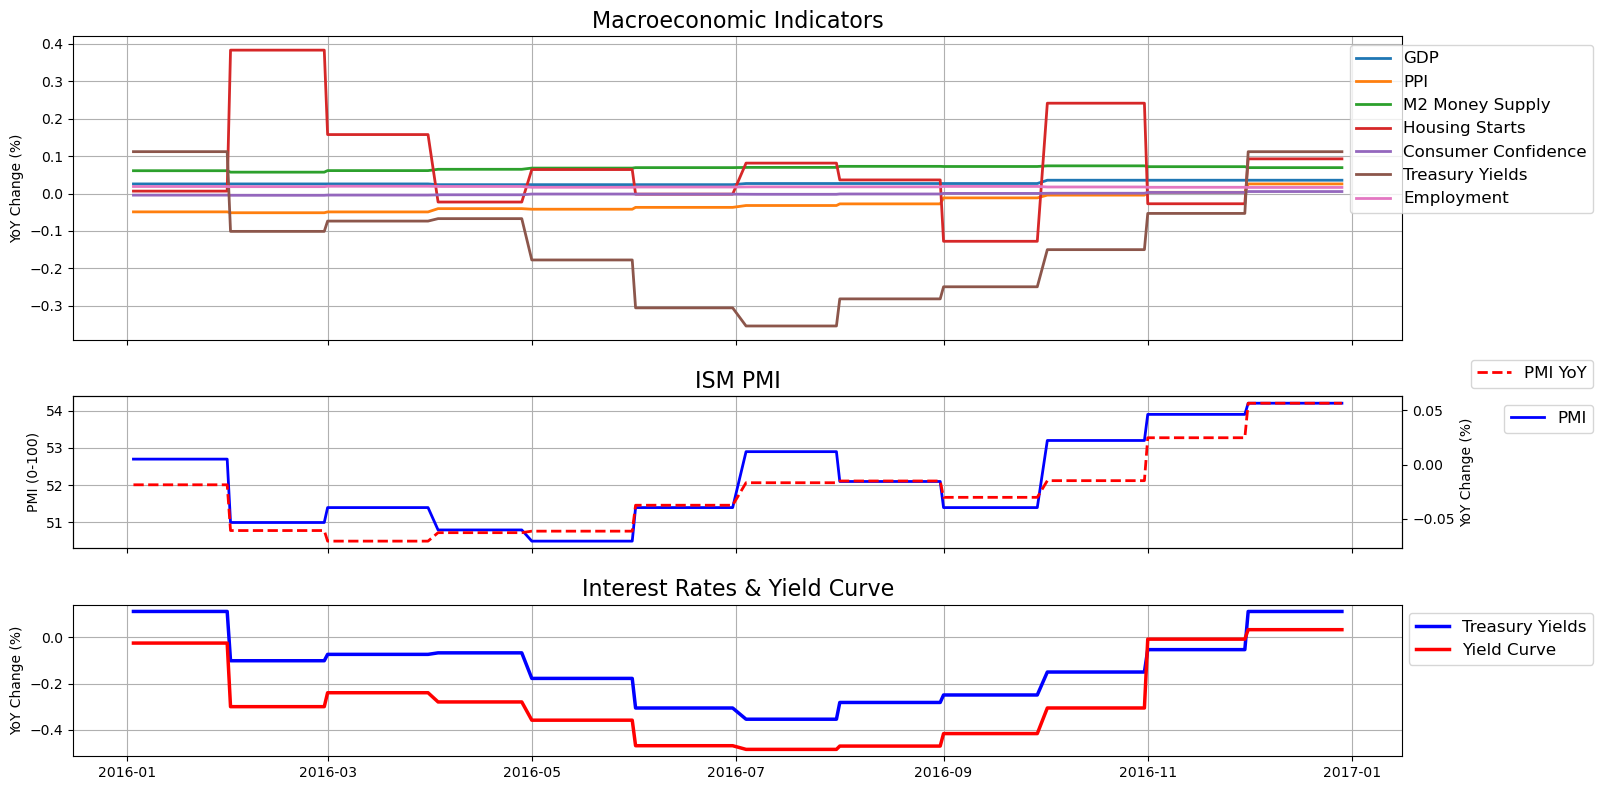
\includegraphics[width=1\linewidth]{judge_reviews/GOOGL_M_gpt-4o-mini/2017-01-01/judge_Macroeconomic_Indicators.png}
    \caption{Macroeconomic}
\end{figure}

\begin{figure}[H]
    \centering
    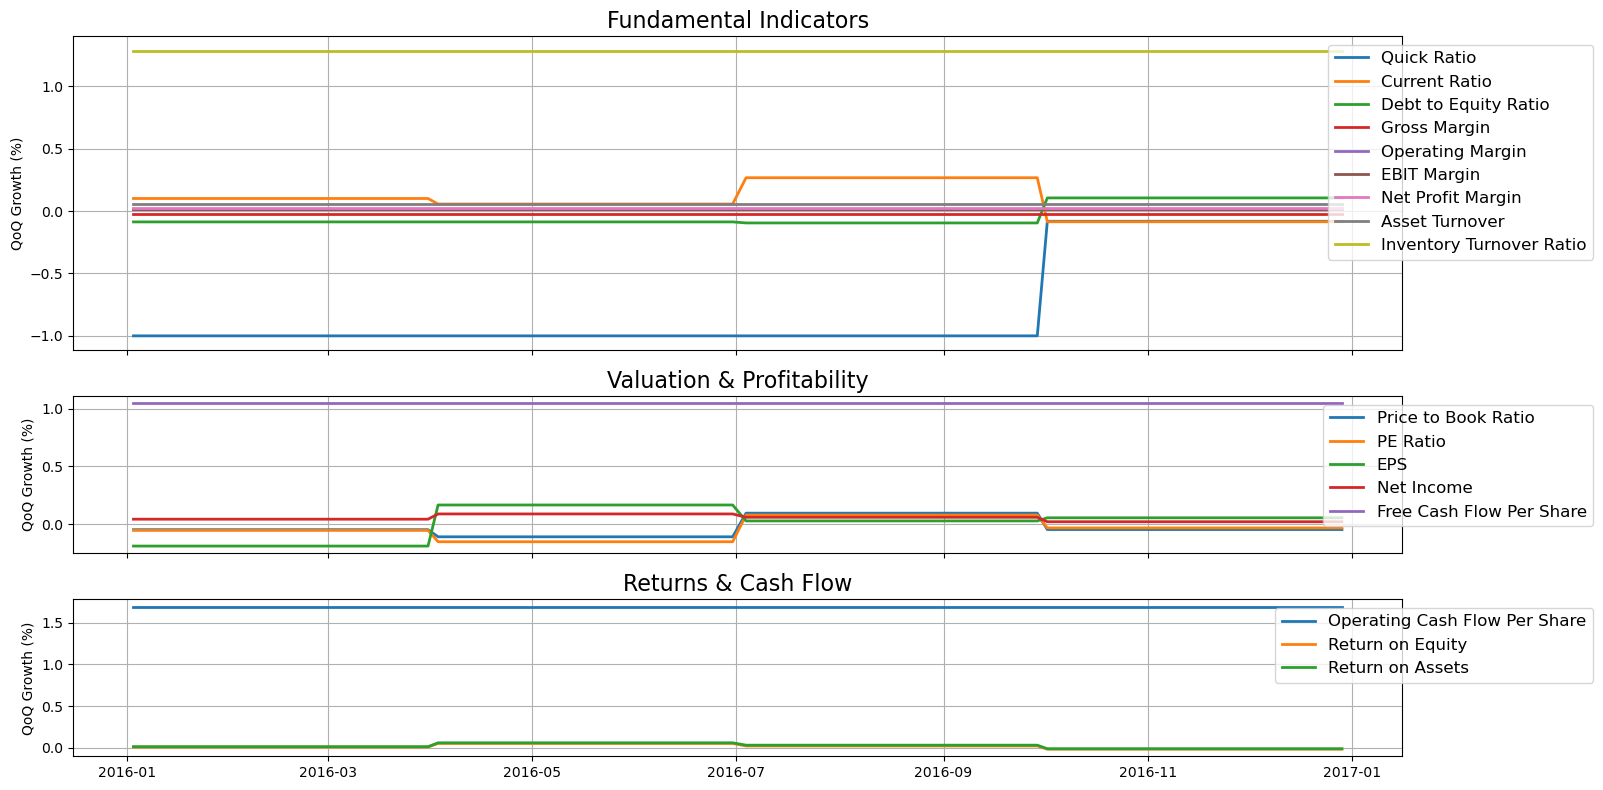
\includegraphics[width=1\linewidth]{judge_reviews/GOOGL_M_gpt-4o-mini/2017-01-01/judge_Fundamental_Indicators.png}
    \caption{Fundamentals}
\end{figure}

\subsection*{Historic 1 Month News}

\textbf{Tech Summit Participation and Market Sentiment}
THE COMPANY's participation in a high-profile technology summit hosted by government officials was seen as a significant opportunity for collaboration on innovation and job creation. However, concerns arose over the selective nature of attendees, leading to speculation about favoritism. Market sentiment towards THE COMPANY remained stable, though some investors questioned potential regulatory risks stemming from government involvement.

\textbf{Increased Competition in the Industry}
A major competitor of THE COMPANY announced advancements in self-driving technology, boasting extensive real-world testing data. Analysts highlighted that while THE COMPANY has been a leader in the space, increased competition could impact its market share and long-term profitability. The news led to mixed reactions, with some investors confident in THE COMPANY’s ability to maintain its lead, while others expressed caution.

\textbf{Speculation on Strategic Partnerships and Buyouts}
Rumors emerged regarding a potential acquisition involving THE COMPANY, sparking volatility in its stock price. While no official confirmation was provided, analysts speculated on the strategic value of such a deal. Some investors saw the speculation as a sign of THE COMPANY's attractiveness in the market, while others remained skeptical about the feasibility of a merger.

\textbf{Increased Focus on Artificial Intelligence Development}
THE COMPANY announced increased investments in artificial intelligence and automation, reinforcing its commitment to future growth in the technology sector. Analysts viewed this as a positive move, particularly as competitors ramped up their own AI initiatives. However, concerns remained regarding the potential regulatory scrutiny and ethical implications of expanded AI deployment.

\textbf{Consumer Data and Privacy Concerns}
Reports surfaced regarding THE COMPANY's collection and usage of consumer data, leading to discussions about privacy regulations and transparency. While THE COMPANY maintained that its practices comply with existing regulations, some analysts warned that growing public and governmental scrutiny could lead to stricter policies, impacting THE COMPANY’s ability to leverage data for competitive advantage.

\newpage

\subsection*{LLMs' Strategy} \label{strategy8}

The traded instrument was GOOGL, with the trading period set between 2017-01-02 and 2017-01-30.

\textbf{LLMs' decision: \textit{LONG}}

\textbf{Rationale}: The analysis suggests a LONG position due to several bullish indicators. Firstly, the company’s technical metrics are showing positive momentum, with the stock price trading above its 50MA (38.22) and maintaining stability above the 200MA. Recent weekly returns also indicate recovery trends, with a reversal from previous declines.

Secondly, fundamental indicators show solid growth potential: EPS YoY growth at 2.7\% and Free Cash Flow YoY exceeding 100\% reflect a strong financial position and operational efficiency.

Furthermore, macroeconomic conditions are favorable, with GDP growth (1\%) and PMI values above 50, suggesting an expanding economy. Analysts’ sentiment remains positive, with price target revisions reflecting confidence in THE COMPANY’s revenue trajectory.

\textbf{Top weighted features influencing this decision}:
\begin{enumerate}
    \item Stock\_Data.Price.Close (38.22)
    \item Technical\_Analysis.RSI.Value (39)
    \item Fundamental\_Data.Growth\_Metrics.EPS\_YoY (2.7\%)
    \item Fundamental\_Data.Cash\_Flow\_Metrics.Free\_Cash\_Flow\_YoY (>100\%)
    \item News_Factors.Analyst\_Price\_Target\_Increase (Impact Score: 5)
\end{enumerate}

\textbf{Key news impacting this strategy}:
\begin{enumerate}
    \item Market analysts raise price targets for THE COMPANY due to strong performance in digital advertising - Market Impact Score: 5/5
    \item THE COMPANY collaborates with major automotive firms for product integration - Market Impact Score: 4/5
    \item Investment in AI and automation expected to improve future offerings - Market Impact Score: 4/5
    \item Strategic executive appointment raises market confidence in THE COMPANY’s leadership - Market Impact Score: 3/5
    \item Expansion into new product categories expected to drive future revenue growth - Market Impact Score: 3/5
\end{enumerate}

\textbf{LLM Decision Insights}

\begin{longtable}{l c}
\toprule
\textbf{LLM Decision Insights} & \textbf{Value} \\
\midrule
Long Probability & 0.75 \\
Short Probability & 0.25 \\
Perplexity & 1.88728   \\
\midrule
Total Tokens & 13112 \\
Total Cost (USD) & \$0.002181 \\
\bottomrule
\end{longtable}

\subsection*{Following Month Data}

\textbf{Performance Metrics}

\begin{longtable}{l c}
\toprule
\textbf{Metric} & \textbf{Value} \\
\midrule
Sharpe Ratio (Annualized SR) & 0.96102 \\
Portfolio Turnover (PTR) & 0 \\
Maximum Drawdown (MDD) & 0.0503262 \\
Mean Drawdown Duration (MDDur) & 2.75 \\
Cumulative Returns & 0.0128745 \\
\bottomrule
\end{longtable}

\begin{figure}[H]
    \centering
    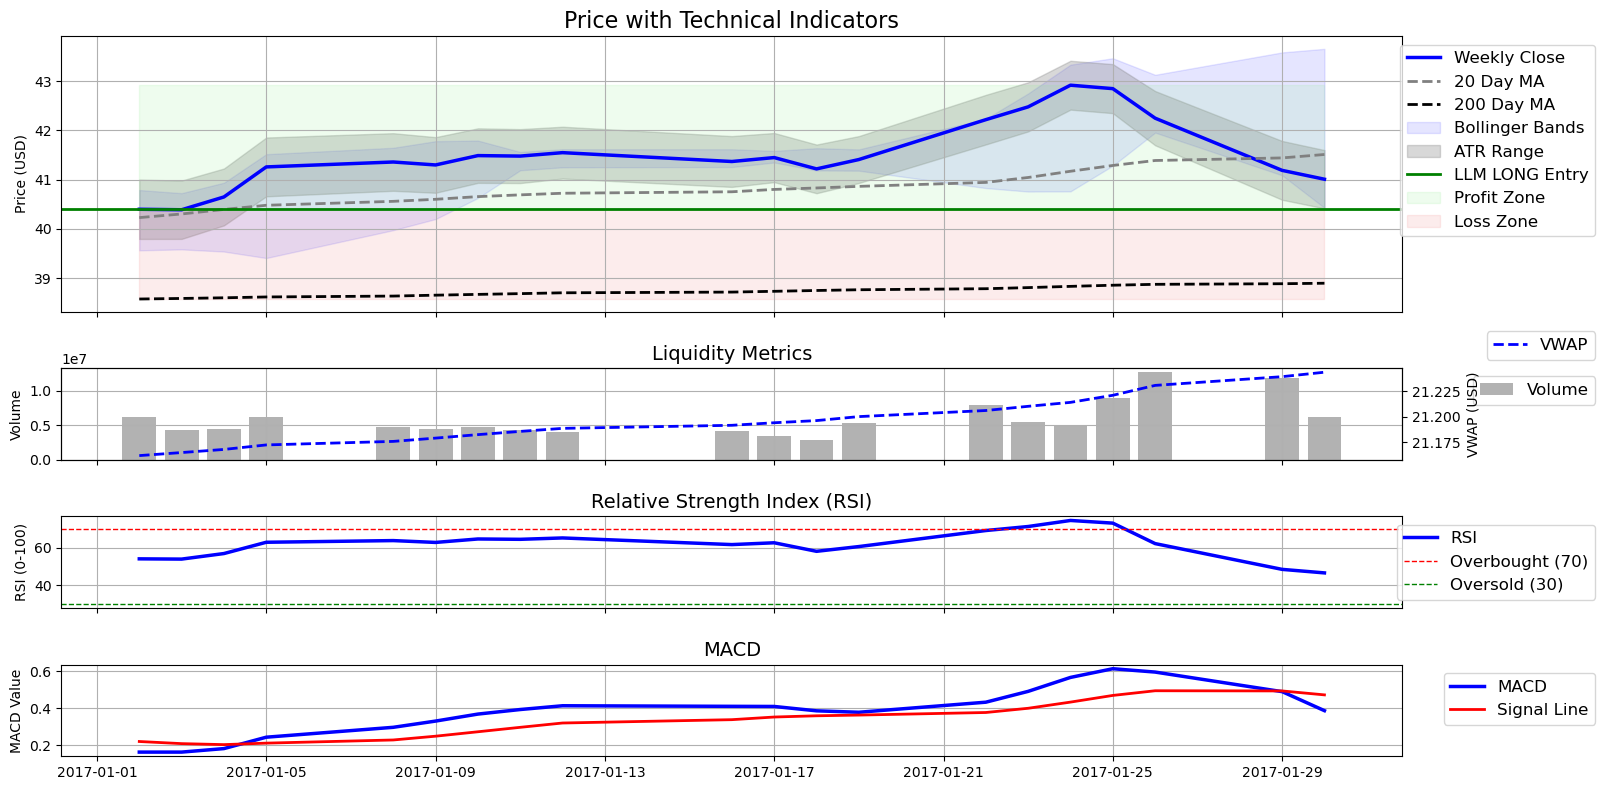
\includegraphics[width=1\linewidth]{judge_reviews/GOOGL_M_gpt-4o-mini/2017-01-01/llm_Price_with_Technical_Indicators.png}
    \caption{Price after LLM's decision}
\end{figure}

\begin{figure}[H]
    \centering
    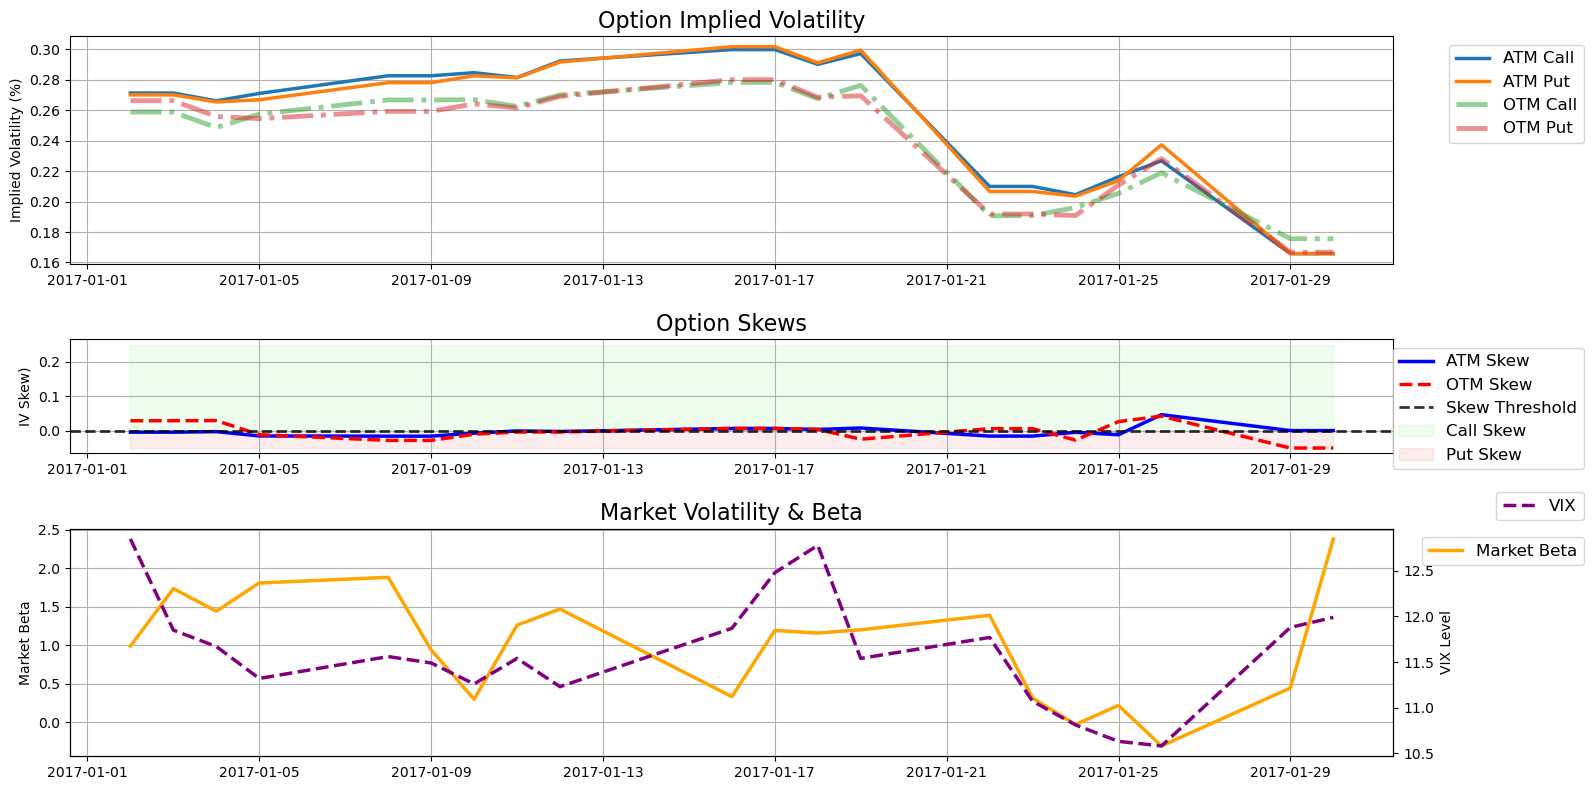
\includegraphics[width=1\linewidth]{judge_reviews/GOOGL_M_gpt-4o-mini/2017-01-01/llm_Market_Volatility_&_Beta.png}
    \caption{Volatility after LLM's decision}
\end{figure}

\begin{tcolorbox}[colback=blue!10, colframe=blue!60, title=\textbf{TASKS}, sharp corners=southwest]
\begin{enumerate}
    \item Fill in the Expert Scoring \textit{rubric}.
    \item If applicable, provide \textit{examples} to correct the strategy.
\end{enumerate}
\end{tcolorbox}
\newpage


\section*{LLM Strategy 9 - No News Analyst Agent}
\label{app:s9}

In this ensemble, only the strategist and the evaluator agents were enabled.

\subsection*{Historic 1 Year Data}

\begin{figure}[H]
    \centering
    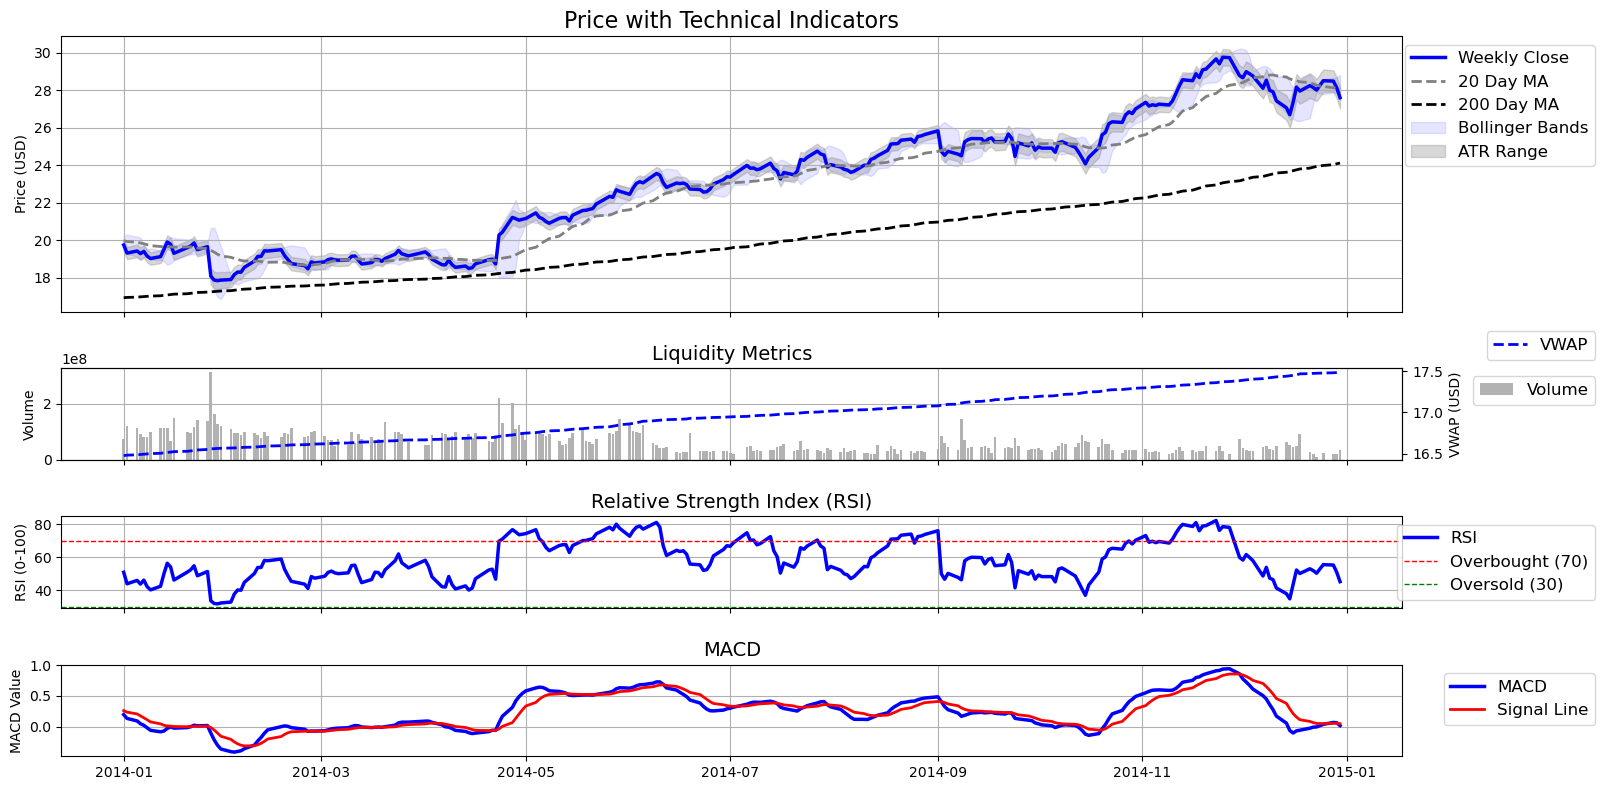
\includegraphics[width=1\linewidth]{judge_reviews/AAPL_M_gpt-4o-mini//2015-01-01/judge_Price_with_Technical_Indicators.png}
    \caption{Price and Technicals}
\end{figure}

\begin{figure}[H]
    \centering
    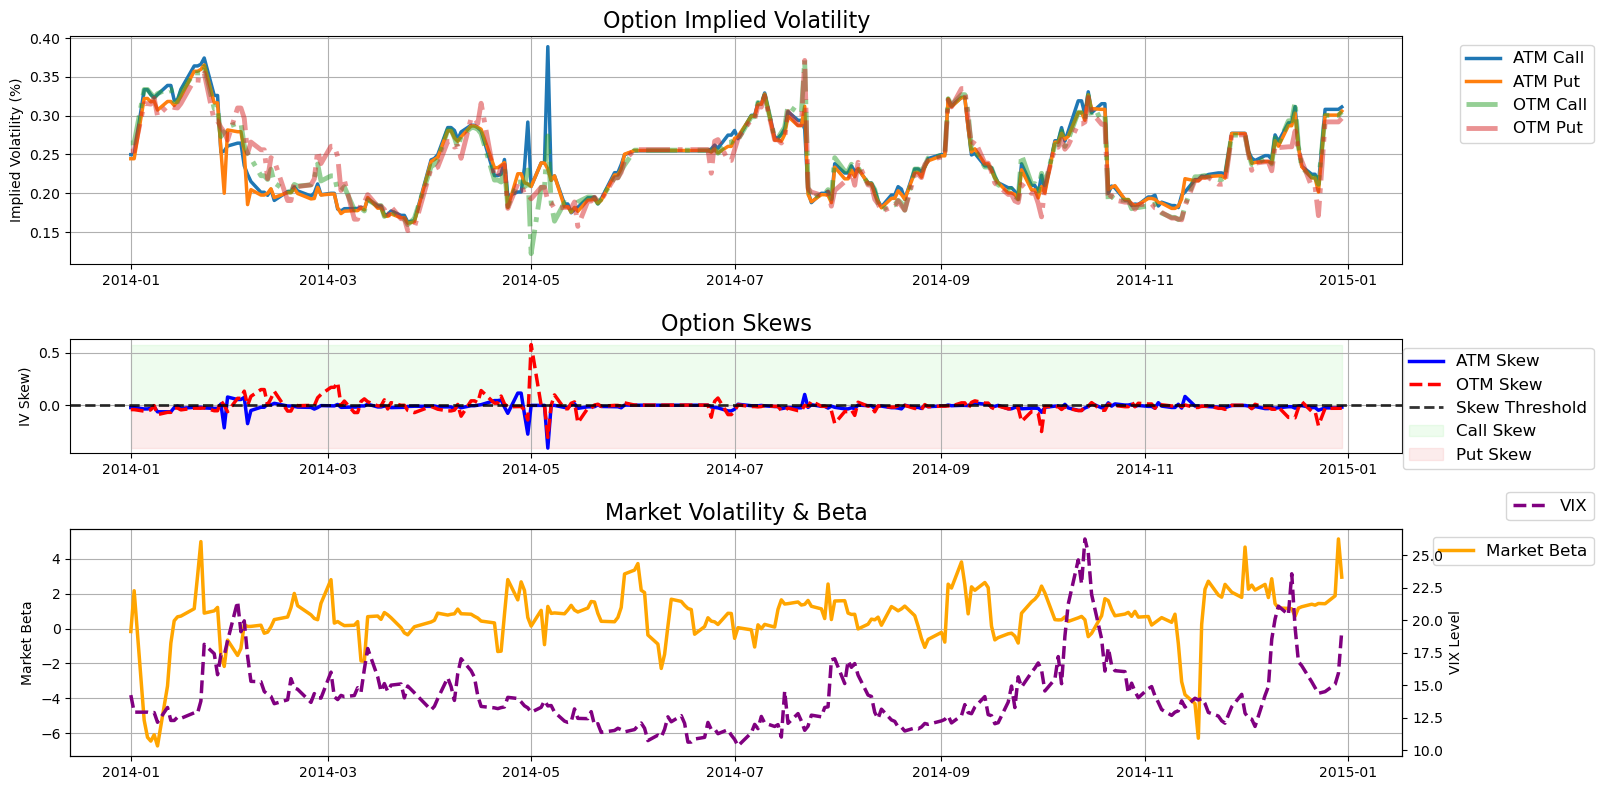
\includegraphics[width=1\linewidth]{judge_reviews/AAPL_M_gpt-4o-mini/2015-01-01/judge_Option_Implied_Volatility.png}
    \caption{Options}
\end{figure}

\begin{figure}[H]
    \centering
    \includegraphics[width=1\linewidth]{judge_reviews/AAPL_M_gpt-4o-mini/2015-01-01/judge_Macroeconomic_Indicators.png}
    \caption{Macroeconomic}
\end{figure}

\begin{figure}[H]
    \centering
    \includegraphics[width=1\linewidth]{judge_reviews/AAPL_M_gpt-4o-mini/2015-01-01/judge_Fundamental_Indicators.png}
    \caption{Fundamentals}
\end{figure}


\subsection*{Historic 1 Month News}

The News Analyst agent was disabled for this sample.

\begin{tcolorbox}[colback=blue!10, colframe=blue!60, title=\textbf{TASKS}, sharp corners=southwest]
\begin{enumerate}
    \item Guess the action to take: \textit{LONG} or \textit{SHORT}.
    \item Write a 1-2 sentence \textit{explanation} on why you decided the action above.
\end{enumerate}
\end{tcolorbox}

\textbf{NEXT PAGE}: Model's Decision and Rationale.

\newpage

\subsection*{LLMs' Strategy} \label{strategy9}

The traded instrument was AAPL, with the trading period set in between 2015-01-05 and 2015-02-02.

\textbf{LLMs' decision: \textit{LONG}}

\textbf{Rationale}: The decision to go LONG is supported by several compelling factors. Firstly, the stock's price at \$28.66 is above both the 20MA (\$28.41) and 50MA (\$26.63), indicating strong bullish momentum and a positive trend in price action. Additionally, the RSI at 58 suggests that while not overbought, there is room for further upward movement without immediate correction risk.

Moreover, recent news highlights record quarterly revenue growth of \$74.6 billion exceeding analyst expectations, which enhances investor confidence and positions the company favorably in the market (Market Impact Score: 5). The analysts' upgrades to their price targets reinforce this sentiment (Market Impact Score: 4). Furthermore, strong sales growth of 70\% in China indicates robust demand and a significant opportunity for future revenue increases.

From a technical perspective, despite some concerns about smartphone sales slowing down, overall growth metrics such as EPS YoY at approximately 48\%, Free Cash Flow YoY at around 58\%, alongside healthy margins (Gross Margin: ~39\%, Net Profit Margin: ~24\%), indicate solid profitability and sustainability.

Additionally, macroeconomic indicators show positive trends with GDP QoQ up and PMI above neutral (53.7), suggesting economic expansion which typically supports equity performance.

\textbf{Top weighted features influencing this decision}:
\begin{enumerate}
    \item Stock\_Data.Price.Close (28.66)
    \item Technical\_Analysis.20MA (28.41)
    \item Technical\_Analysis.50MA (26.63)
    \item Fundamental\_Data.Growth\_Metrics.EPS\_YoY (48\%)
    \item Fundamental\_Data.Growth\_Metrics.Free\_Cash\_Flow\_YoY (58\%)
\end{enumerate}

\textbf{Key news impacting this strategy}:
\begin{enumerate}
    \item Record quarterly revenue of \$74.6 billion - Market Impact Score: 5/5
    \item Analysts raised price targets following strong earnings - Market Impact Score: 4/5
    \item Anticipated launch of Apple Watch as new revenue stream - Market Impact Score: 4/5
    \item Strong revenue growth in China (70\%) - Market Impact Score: 4/5
    \item Concerns over potential slowing smartphone sales growth - Market Impact Score: 3/5
\end{enumerate}

\textbf{LLM Decision Insights}

\begin{longtable}{l c}
\toprule
\textbf{LLM Decision Insights} & \textbf{Value} \\
\midrule
Long Probability & 0.78 \\
Short Probability & 0.22 \\
Perplexity & 5.89012e+15 \\
\midrule
Total Tokens & 63630 \\
Total Cost (USD) & \$0.009766 \\
\bottomrule
\end{longtable}

\subsection*{Following Month Data}

\textbf{Performance Metrics}

\begin{longtable}{l c}
\toprule
\textbf{Metric} & \textbf{Value} \\
\midrule
Sharpe Ratio (Annualized SR) & 4.17844 \\
Portfolio Turnover (PTR) & 0 \\
Maximum Drawdown (MDD) & 0.0535714 \\
Mean Drawdown Duration (MDDur) & 2.77778 \\
Cumulative Returns & 0.116297 \\
\bottomrule
\end{longtable}

\begin{figure}[H]
    \centering
    \includegraphics[width=1\linewidth]{judge_reviews/AAPL_M_gpt-4o-mini//2015-01-01/llm_Price_with_Technical_Indicators.png}
    \caption{Price after LLM's decision}
\end{figure}

\begin{figure}[H]
    \centering
    \includegraphics[width=1\linewidth]{judge_reviews/AAPL_M_gpt-4o-mini/2015-01-01/llm_Market_Volatility_&_Beta.png}
    \caption{Volatility after LLM's decision}
\end{figure}

\begin{tcolorbox}[colback=blue!10, colframe=blue!60, title=\textbf{TASKS}, sharp corners=southwest]
\begin{enumerate}
    \item Fill in the Expert Scoring \textit{rubric}.
    \item If applicable, provide \textit{examples} to correct the strategy.
\end{enumerate}
\end{tcolorbox}
\newpage


\section*{LLM Strategy 10}
\label{app:s10}

In this ensemble, only the strategist agent is active, the news analyst and the evaluator were disabled.

\subsection*{Historic 1 Year Data}

\begin{figure}[H]
    \centering
    \includegraphics[width=1\linewidth]{judge_reviews//META_M_gpt-4o-mini//2016-01-01/judge_Price_with_Technical_Indicators.png}
    \caption{Price and Technicals}
\end{figure}

\begin{figure}[H]
    \centering
    \includegraphics[width=1\linewidth]{judge_reviews/META_M_gpt-4o-mini/2016-01-01/judge_Option_Implied_Volatility.png}
    \caption{Options}
\end{figure}

\begin{figure}[H]
    \centering
    \includegraphics[width=1\linewidth]{judge_reviews/META_M_gpt-4o-mini/2016-01-01/judge_Macroeconomic_Indicators.png}
    \caption{Macroeconomic}
\end{figure}

\begin{figure}[H]
    \centering
    \includegraphics[width=1\linewidth]{judge_reviews/META_M_gpt-4o-mini/2016-01-01/judge_Fundamental_Indicators.png}
    \caption{Fundamentals}
\end{figure}

\subsection*{Historic 1 Month News}

The News Analyst agent was disabled for this sample.

\begin{tcolorbox}[colback=blue!10, colframe=blue!60, title=\textbf{TASKS}, sharp corners=southwest]
\begin{enumerate}
    \item Guess the action to take: \textit{LONG} or \textit{SHORT}.
    \item Write a 1-2 sentence \textit{explanation} on why you decided the action above.
\end{enumerate}
\end{tcolorbox}
\textbf{NEXT PAGE}: Model's Decision and Rationale.

\newpage

\subsection*{LLMs' Strategy} \label{strategy10}

The traded instrument was META, with the trading period set between 2016-01-04 and 2016-02-01.

\textbf{LLMs' decision: \textit{SHORT}}

\textbf{Rationale}: The stock exhibits several red flags indicating a potential decline. Firstly, the negative EBIT Margin (-0.1333) and Negative Net Profit Margin (-0.1278) suggest that the company is currently operating at a loss, which can deter investors and decrease demand for shares.

Additionally, the Current Ratio (0.1962) and Quick Ratio (0.0) indicate severe liquidity issues, implying that the company may struggle to cover its short-term liabilities, further increasing financial risk.

From a technical perspective, both RSI values (35.94), which is below 40 suggests weak momentum while MACD shows bearish signals with a drop in strength over recent periods (-0.0248). The stock price has also been trading well below its moving averages: 20MA (approx 269), 50MA (approx 334), suggesting downward pressure on price action.

Given these factors coupled with high volatility indicated by ATR of approximately 0.0225 points towards potential price swings unfavorable to long positions; thus establishing a short position could be beneficial in capturing downside movement over the next month.

\textbf{LLM Decision Insights}

The evaluator agent was disabled, these insights are not precise.

\begin{longtable}{l c}
\toprule
\textbf{LLM Decision Insights} & \textbf{Value} \\
\midrule
Long Probability & 0.4 \\
Short Probability & 0.6 \\
Perplexity & 5.21024e+14   \\
\midrule
Total Tokens & 2625 \\
Total Cost (USD) & \$0.000540 \\
\bottomrule
\end{longtable}

\subsection*{Following Month Data}

\textbf{Performance Metrics}

\begin{longtable}{l c}
\toprule
\textbf{Metric} & \textbf{Value} \\
\midrule
Sharpe Ratio (Annualized SR) & 0.98081 \\
Portfolio Turnover (PTR) & 0 \\
Maximum Drawdown (MDD) & 0.329518 \\
Mean Drawdown Duration (MDDur) & 8.05882 \\
Cumulative Returns & 0.0222242 \\
\bottomrule
\end{longtable}


\begin{figure}[H]
    \centering
    \includegraphics[width=1\linewidth]{judge_reviews/META_M_gpt-4o-mini//2016-01-01/llm_Price_with_Technical_Indicators.png}
    \caption{Price after LLM's decision}
\end{figure}

\begin{figure}[H]
    \centering
    \includegraphics[width=1\linewidth]{judge_reviews/META_M_gpt-4o-mini/2016-01-01/llm_Market_Volatility_&_Beta.png}
    \caption{Volatility after LLM's decision}
\end{figure}

\begin{tcolorbox}[colback=blue!10, colframe=blue!60, title=\textbf{TASKS}, sharp corners=southwest]
\begin{enumerate}
    \item Fill in the Expert Scoring \textit{rubric}.
    \item If applicable, provide \textit{examples} to correct the strategy.
\end{enumerate}
\end{tcolorbox}
\newpage


\end{document}
